\documentclass[10pt,a4paper,cours]{nsi}
\usepackage{circuitikz}
\begin{document}


% \part{Représentation\\ de l'information}

% \chapter{Bases de numération}
\introduction{Partons sur de bonnes bases.}


On note $\N$ l'ensemble des \textit{entiers naturels} : $\N=\lbrace 0;1;2;\ldots\rbrace$.\\

Nous avons l'habitude d'utiliser la base 10 pour représenter les entiers naturels, c'est-à-dire qu'on utilise 10 symboles, appelés \textit{chiffres}
pour les écrire : 0, 1, 2, \ldots, 9.
Or il n'en a pas toujours été ainsi :
\begin{itemize}
    \item 	au \textsc{I}\er millénaire av. J.-C., les Babyloniens utilisaient la base soixante pour mesurer le temps et les angles ;
    \item 	durant le \textsc{I}\er millénaire, les Mayas et les Aztèques se servaient de la base vingt (et d'ailleurs en France, 80 se lit «
          quatre-vingts» ) ;
    \item 	entre le \textsc{vii}\eme et le \textsc{xv}\eme siècle, les astronomes arabes utilisaient la base cent cinquante pour élaborer des tables
          permettant de trouver la position d'un astre dans le ciel à un moment donné.
\end{itemize}
De nos jours, en Informatique, on utilise beaucoup la base deux, dite \textit{binaire} et la base seize, appelée \textit{hexadécimale}.\\
L'objectif de ce chapitre est de donner les méthodes permettant d'écrire un entier naturel dans une base donnée, plus précisément dans les bases 2,
10 et 16. Nous verrons également comment passer facilement du binaire à l'hexadécimal et vice-versa.

\section{\'Ecriture binaire d'un entier naturel}
\subsection{Pourquoi le binaire ?}


\floatpictureleft{0.2}{ch-bases/img/joke1}{
    Pour simplifier, disons qu'au niveau le plus « bas »  d'un ordinateur, se trouvent des (millions de) transistors
    qui jouent chacun un rôle d'interrupteur. De multiples points de l'ordinateur peuvent alors être soumis à une tension
    (état 1) ou non (état 0).
    En considérant 2 de ces points, on voit que l'état de ce système peut être 00, 01, 10 ou 11. Cela fait 4 possibilités
    et le binaire est né !
}
\subsection{Comprendre l'écriture en base 2}

Puisqu'il n'y a que deux chiffres en binaire, compter est simple mais nécessite rapidement plus de chiffres qu'en base
10 :\\

\begin{center}
    \alternaterowcolors
    \begin{tabular}{CCCCCCCCCCC}

        \textbf{\'Ecriture décimale} & 0 & 1 & 2  & 3  & 4   & 5   & 6   & 7   & 8    & \dots \\

        \textbf{\'Ecriture binaire}  & 0 & 1 & 10 & 11 & 100 & 101 & 110 & 111 & 1000 & \dots \\
    \end{tabular} \\[1em]
\end{center}

\begin{notation}
    On écrira $(11)_{10}$ pour insister sur le fait qu'on parle du nombre 11 \textit{en base 10}, et $(11)_2$ pour dire que c'est une écriture
    binaire.\\
    Lorsque ce n'est pas précisé cela veut dire que l'écriture est en base 10.\\
    Ainsi $(11)_2=3$, et de même, $(111)_2=7$.\\
\end{notation}


Tout entier naturel admet une unique écriture décimale (c'est-à-dire en base 10), il en va de même en binaire:
\begin{propriete}[ : écriture binaire d'un entier naturel]
    Tout entier naturel possède une unique écriture en base 2, dite \textit{écriture binaire}.
    Plus précisément, soit $n\in\N$, alors il existe un unique entier $k\in\N$ et $k+1$ nombres $a_i$, uniques et valant 0
    ou 1 et tels que $$n=a_02^0+a_12^1+\ldots+a_k2^k$$
    ce qui s'écrit aussi
    $$n=\sum_{i=0}^ka_i2^i$$
\end{propriete}
\begin{exemple}
    Lorsqu'on regarde le tableau précédent, on voit que $6=(110)_2$.\\Cela s'interprète ainsi :\\

    \alternaterowcolors
    \begin{tabular}{CCCC}
        Chiffre binaire & 1     & 1     & 0     \\
        Valeur          & $2^2$ & $2^1$ & $2^0$ \\
    \end{tabular}\ \ \ et on obtient $6=0\times 2^0+1\times 2^1+1\times 2^2$.
\end{exemple}

\begin{methode}[ 1 : passer de la base 2 à la base 10]
    Que vaut $(11101)_2$ ?
    \begin{center}
        \alternaterowcolors[UGLiPurple]
        \begin{tabular}{CCCCCC}
            Chiffre binaire & 1     & 1     & 1     & 0     & 1     \\
            Valeur          & $2^4$ & $2^3$ & $2^2$ & $2^1$ & $2^0$ \\
        \end{tabular}
    \end{center}
    \begin{tabbing}
        $(11101)_2$	\= 	$=1\times 2^4+1\times 2^3+1\times 2^2+0\times 2^1+1\times 2^0$	\\
        \>	$=16+8+4+1$	\\
        \>	$=29$
    \end{tabbing}\nopagebreak
\end{methode}

\begin{methode}[ 2 : passer de la base 10 à la base 2]
    Comprenons ce que veut dire une écriture décimale :
    \begin{tabbing}
        $203$	\= 	$=200+3$	\\

        \>	$=2\times 10^2+0\times 10^1+3\times 10^0$
    \end{tabbing}
    Faisons la même chose en base 2 :
    \begin{tabbing}
        $203$	\= 	$=128+64+8+2+1$	\\

        \>	$=2^7+2^6+2^3+2^1+2^0$	\\

        \>	$=1\times 2^7+1\times 2^6+0\times 2^5 + 0\times 2^4 +1\times 2^3+0\times 2^2 + 1\times
            2^1+1\times 2^0$	\\

        \> $=(11001011)_2$
    \end{tabbing}
    Cette méthode est pratique quand l'entier est petit et que l'on connaît bien les premières puissances de deux.\\
    Quand ce n'est pas le cas, une autre méthode (la méthode 3) peut être employée.

\end{methode}
\'Evidemment, \textsc{Python} connait le binaire et travaille avec des valeurs entières de type \mintinline{python}{int} (\textit{integer} veut dire « entier » en Anglais, pour plus de précisions, voir le chapitre \ref{ch:valeurs}, partie \ref{sec:int} ).\\
Voici comment écrire un \mintinline{python}{int} en binaire et comment obtenir l'écriture
binaire d'un \mintinline{python}{int}.
\begin{pys}
    \begin{minted}{python}
        >>> 0b11001011 # faire précéder le nombre de 0b
        203
        >>> bin(29)
        '0b11101'
    \end{minted}
\end{pys}

\subsection{Un algorithme pour déterminer l'écriture binaire d'un entier naturel}
\begin{methode}[ 3 : les divisions successives]
    Voici comment on trouve les chiffres de l'écriture \textit{décimale} de 203 :\\

    On divise 203 par 10, cela fait 20, il reste 3, c'est le chiffre des unités.\\
    On recommence avec 20, on le divise par 10, cela fait 2, reste 0, chiffre des dizaines.\\
    On continue, on divise 2 par 10, cela fait 0, reste 2, chiffre des des centaines.\\
    Puisqu'on a trouvé un quotient de 0, on s'arrête.\\
    On peut écrire cela simplement :
    $$\division[10]{203}$$
    Voici maintenant comment on trouve son écriture binaire. On procède comme en base 10 mais en divisant par 2 :
    $$\division[2]{203}$$

    On a donc successivement établi :
    \begin{tabbing}
        203	\= 	$=101\times 2 +1$	\\
        \>	$=(50\times 2 +1)\times 2+1  $	\\
        \>	$=((25\times 2 +0)\times 2 +1)\times 2+1  $	\\
        \>	$=(((12\times 2 +1)\times 2 +0)\times 2 +1)\times 2+1  $	\\
        \>	$=((((6\times 2 +0)\times 2 +1)\times 2 +0)\times 2 +1)\times 2+1  $	\\
        \>	$=(((((3\times 2 +0)\times 2 +0)\times 2 +1)\times 2 +0)\times 2 +1)\times 2+1  $	\\
        \>	$=((((((1\times 2 +1)\times 2 +0)\times 2 +0)\times 2 +1)\times 2 +0)\times 2 +1)\times 2+1  $	\\

        \>	$=1\times 2^7+1\times 2^6+0\times 2^5 + 0\times 2^4 +1\times 2^3+0\times 2^2 + 1\times 2^1+1\times
            2^0$\\
        \> $=(11001011)_2$
    \end{tabbing}
    Cette succession d'égalités n'est (heureusement) pas à écrire à chaque fois.

\end{methode}

Les trois méthodes précédentes se programment facilement et la dernière est de loin la plus courte à écrire.

\subsection{Vocabulaire}

\floatpictureleft{0.4}{ch-bases/img/bitjoke}{
    Un chiffre décimal peut être 0, 1, 2, 3, 4, 5, 6, 7, 8 ou 9.\\
    Un chiffre binaire peut être seulement 0 ou 1. En Anglais, \textit{chiffre binaire} se traduit par \textit{binary digit},
    que l'on abrège en \textit{bit}. On garde cette dénomination en Français.\\
    Le bit est « le plus petit morceau d'information numérique » .
}\medskip\par
Pour les écrire, on regroupe les chiffres décimaux par paquets de 3, comme dans \np{1230014} par exemple.
En binaire on groupe les bits par 4, on écrira donc $17=\left(1\ 0001\right)_2$.\\
La plupart du temps, en machine, les bits sont groupés par 8 (deux paquets de 4). Un tel paquet s'appelle un \textit{octet}, et on écrit donc des \textit{mots binaires} de longueur 8 tels que $0000\ 0011$ : l'octet représente ici le nombre 3. Les bits à zéros ne sont pas inutiles.\\

Lorsqu'on considère un nombre écrit en binaire, on parle souvent de \textit{bit de poids fort} et de
\textit{bit de poids faible} pour parler respectivement du bit associé à la plus grande puissance de 2, et du bit
d'unités.\\
Considérons l'octet $(0010\ 0101)_2$. Son bit de poids fort est 0, son bit de poids faible est 1.

\section{\'Ecriture hexadécimale d'un entier naturel}

La base « naturelle »  de l'informatique est la base 2, mais elle n'est pas très pratique car elle donne lieu à
des écritures trop longues.
La base 10 nous paraît bien meilleure parce que nous avons l'habitude de l'utiliser, mais elle ne fait pas bon ménage
avec la base 2 : il n'y a pas de méthode simple pour passer du décimal au binaire, et vice versa.\\
La base 16, ou base \textit{hexadécimale}, est en revanche très adaptée à l'écriture des paquets de 4 bits, et par
extension à celle des octets et autres écritures binaires.\\

En hexadécimal, on dispose de 16 chiffres : 0, 1, 2, 3, 4, 5, 6, 7, 8, 9, A, B, C, D, E et F.

\begin{propriete}[ : écriture binaire d'un entier naturel]
    Tout entier naturel possède une unique écriture en base 16, dite \textit{écriture hexadécimale}.
    Plus précisément, soit $n\in\N$, alors il existe un unique entier $k\in\N$ et $k+1$ nombres $a_i$, uniques et valant 0, 1, 2, \ldots, ou F et tels
    que $$n=a_016^0+a_16^1+\ldots+a_k16^k$$
    ce qui s'écrit aussi
    $$n=\sum_{i=0}^ka_i16^i$$
\end{propriete}

\begin{remarque}
    On a vu une propriété similaire en base 2 et en fait elle est valable \textit{dans toutes les bases}  $b$ (où $b$ est un entier naturel supérieur ou
    égal à 2). Cela justifie par exemple l'utilisation de la base 20 ou de la base 150.
\end{remarque}

Les méthodes que l'on a vu en base 2 et 10 se transposent en base 16.
\begin{methode}[ 4 : passer de la base 16 à la base 10]
    Déterminons l'écriture décimale de $(D4A)_{16}$ :
    \begin{tabbing}
        $(D4A)_{16}$  	\= $=13\times 16^2 + 4\times 6 + 10\times 16^0$	 car D vaut 13 et A vaut 10.\\
        \>	$=3402$
    \end{tabbing}
\end{methode}
\begin{methode}[ 5 : passer de la base 10 à la base 16]
    Déterminons maintenant l'écriture hexadécimale de 503:

    $503 = 31 \times 16 + \underline{7}$.\\

    $31 = 1\times 16 + \underline{15}$ et 15 s'écrit $\underline{F}$.\\

    $1 = {\boldmath 0}\times 16 + \underline{1}$ et on arrête car le quotient est nul.\\

    $503=(1F7)_{16}$.\\

\end{methode}
\begin{figure}[H]
    \begin{center}
        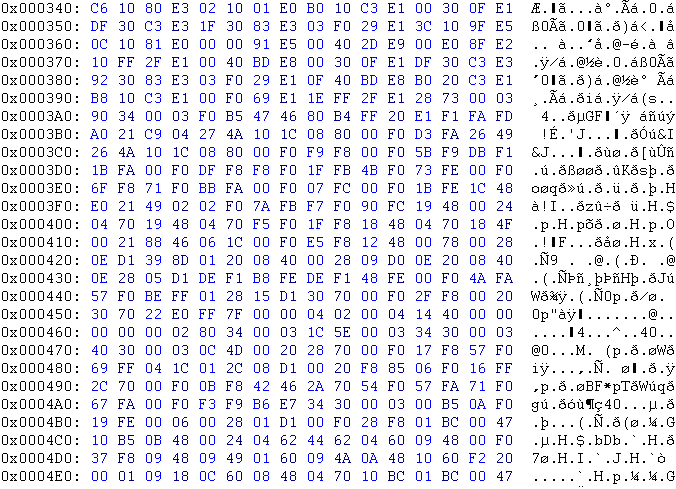
\includegraphics[width=12cm]{ch-bases/img/hex.png}\\
        \caption*{Un éditeur hexadécimal montre le contenu d'un fichier, d'un disque dur, ou de la RAM d'un ordinateur. La première colonne indique l'adresse,
            puis 16 octets écrits en hexadécimal et enfin les caractères correspondants.}
    \end{center}
\end{figure}
\section{Hexadécimal et binaire : un mariage heureux}
Le grand avantage qu'apporte l'hexadécimal s'illustre facilement :

\begin{methode}[ 6 : passer de la base 2 à la base 16]
    \begin{tabbing}
        $(101101000011101)_2$	\=	$=(0101\ 1010\ 0001\ 1101)_2$\\
        \>	$=\left(\underbrace{0101}_5\ \underbrace{1010}_A\ \underbrace{0001}_1\ \underbrace{1101}_D\right)_2$\\
        \>	$=(5A1D)_{16}$
    \end{tabbing}
\end{methode}

\begin{methode}[ 7 : passer de la base 16 à la base 2]
    $(F7B)_{16}=\left(\underbrace{1111}_F\ \underbrace{0111}_7\ \underbrace{1011}_B\right)_2$
\end{methode}
\begin{figure}
    \begin{center}
        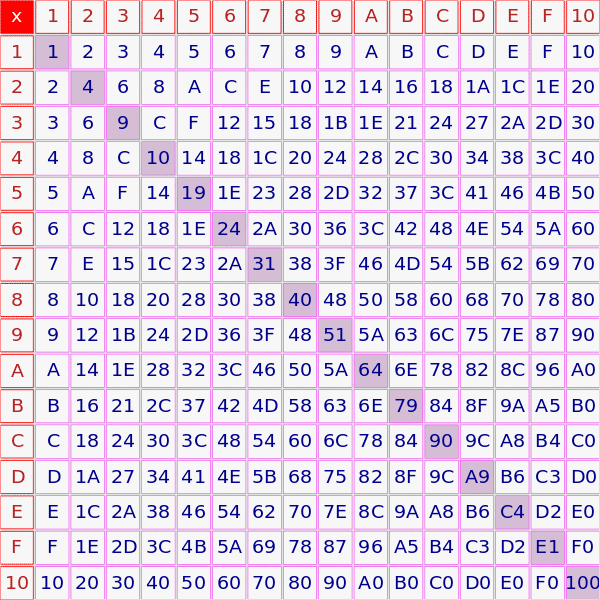
\includegraphics[width=10cm]{ch-bases/img/hexmult.png}\\
        \caption*{Table de multiplication hexadécimale.}
    \end{center}
\end{figure}


\section{Additions}

On pose l'opération à la main : c'est la même chose qu'en base 10.
\subsection*{En base 2}
La seule différence avec la base 10 c'est que deux 1 donnent $(2)_{10}$ donc $(10)_2$, donc un zéro et une retenue de 1.
Quand il y a deux 1 et une retenue de 1 en plus, cela donne $(3)_{10}$ donc $(11)_2$, donc un 1 et une retenue de 1.

\tabulardefault
\begin{exemple}[]
    \begin{center}
        \begin{tabular}{ccccccccc}
              &   &   & $_1$ & $_1$ & $_1$ &   &   &   \\
              & 1 & 1 & 0    & 1    & 0    & 1 & 0 & 1 \\
            + &   &   &      & 1    & 1    & 1 & 0 & 0 \\
            \hline
            = & 1 & 1 & 1    & 1    & 0    & 0 & 0 & 1 \\
        \end{tabular} \\[2em]
    \end{center}
\end{exemple}

\subsection*{En base 16}

C'est encore la même chose. Il faut bien se souvenir de la valeur de A, B, C, D, E et F.\\
Ajouter 8 et 3 ne provoque pas de retenue puisque $8+3=11$ et que $11$ est $B$ en base 16.\\
Dès que l'addition de 2 chiffres dépasse 15, il y aura une retenue : par exemple 9 et A donnent $(19)_{10}$, donc $(13)_{16}$. Ainsi on note 3 et une retenue de 1.

\begin{exemple}
    \begin{center}
        \begin{tabular}{ccccc}
              &   & $_1$ &   &   \\
              & 2 & 4    & 9 & 8 \\
            + & 1 & 7    & A & 3 \\
            \hline
            = & 3 & C    & 3 & B \\
        \end{tabular}
    \end{center}
\end{exemple}



\section{Exercices}

\begin{exercice}
    Donner l'écriture décimale des onze premières puissances de deux.
\end{exercice}

\begin{exercice}
    \begin{enumerate}
        \item 	Calculer $2^6+2^4+2^3+2^0$.
        \item 	En déduire l'écriture binaire de 89.
    \end{enumerate}
\end{exercice}

\begin{exercice}
    \begin{enumerate}
        \item 	Calculer $2^7+2^3+2^2+2^1$.
        \item 	En déduire l'écriture décimale de  $(1000 1110)_2$.
    \end{enumerate}
\end{exercice}

\begin{exercice}[]
    En utilisant la méthode 2, donner l'écriture binaire de
    \begin{enumerate}
        \item 	56
        \item 	35
        \item 	13
    \end{enumerate}
\end{exercice}

\begin{exercice}[]
    En utilisant la méthode 3, donner l'écriture binaire de
    \begin{enumerate}
        \item 	142
        \item 	273
        \item 	1000
    \end{enumerate}
\end{exercice}

\begin{exercice}
    \begin{itemize}
        \item 	Donner l'écriture décimale de $(1101\ 1010)_2$.
        \item 	Donner l'écriture binaire de 2016.
        \item 	Donner l'écriture hexadécimale de 2016.
    \end{itemize}
\end{exercice}

\begin{exercice}
    \begin{itemize}
        \item 	Donner les écritures décimales de $(11)_2$, $(111)_2$, $(1111)_2$.
        \item   Soit $n \in \N$, conjecturer la valeur de $ \left(\underbrace{1\ldots 1}_{n\textrm{ chiffres}}\right)_2$.
    \end{itemize}
\end{exercice}

\begin{exercice}
    Pour multiplier par dix un entier naturel exprimé en base dix, il suffit d'ajouter un 0 à sa
    droite, par exemple, $12\times 10 = 120$.\\
    Quelle est l'opération équivalente pour les entiers naturels exprimés en base deux?
\end{exercice}

\begin{exercice}
    \begin{enumerate}
        \item 	Donner l'écriture binaire de 174.
        \item 	Donner celle de 17.
        \item 	Poser l'addition de 174 et 17 en binaire.
        \item 	Donner l'écriture décimale du résultat et vérifier.
    \end{enumerate}
\end{exercice}

\begin{exercice}
    \begin{enumerate}
        \item 	Donner l'écriture hexadécimale de 1022.
        \item 	Donner celle de 3489.
        \item 	Poser l'addition de 1022 et 3489 en hexadécimal.
        \item 	Donner l'écriture décimale du résultat et vérifier.
    \end{enumerate}
\end{exercice}

\begin{exercice}[*]
    Le Roi d'un pays imaginaire fait frapper sa monnaie par 8 nains : chacun d'entre eux produit des pièces d'or de 10g chacune.\\

    Un jour, son Mage lui annonce : « Majesté, mon miroir magique m'a prévenu que certains de vos nains vous volent. Ils prélèvent 1g d'or sur chaque pièce qu'ils frappent. Pour vous aider à trouver les voleurs, voici une balance magique. Elle est précise au gramme près et peut peser autant que vous voulez. Malheureusement elle ne peut être utilisée qu'une fois.»\\

    Le lendemain, le Roi convoque les 8 nains en demandant à chacun d'apporter un coffre rempli de pièces d'or qu'il a frappées.\\
    On suppose que
    \begin{itemize}
        \item chaque nain dispose d'autant de pièces que nécessaire ;
        \item un nain honnête n'a que des pièces de 10g ;
        \item un nain voleur n'a que des pièces de 9g ;
    \end{itemize}

    Peux-tu aider le Roi pour démasquer les voleurs?
\end{exercice}
% \chapter{Représentation des entiers}
\introduction{Pour tout comprendre, lire ce chapitre en entier.}

Nous avons vu au chapitre précédent comment écrire les entiers naturels en binaire ou en hexadécimal. Maintenant nous allons
étudier comment les entiers \textit{relatifs}, c'est-à-dire positifs ou négatifs (on dit aussi \textit{signés}) sont
représentés en machine.\\
On va d'abord se limiter aux entiers naturels et on va voir qu'il n'y a pas de difficulté majeure à comprendre leur représentation en machine.


\begin{remarque}[ importante]
    Il existe des \textit{centaines} de langages de programmation. Les principaux sont : \textsc{C},  \textsc{C++}, \textsc{C\#}, \textsc{Java},
    \textsc{Python}, \textsc{PHP} et \textsc{Javascript} (cette liste est non exhaustive). Chaque langage utilise ses propres \textit{types de variable}
    mais en général il y a beaucoup de ressemblances. On travaillera donc sur des exemples de types de variables utilisés dans tel ou tel langage\ldots
    sachant que ce type n'existe pas nécessairement en \textsc{Python}.
\end{remarque}

\section{Représentation des entiers naturels :\\ l'exemple du unsigned char}

En Informatique on dit souvent qu'un entier naturel est \textit{non signé} (ou \textit{unsigned} en anglais). Le type \mintinline{c}{unsigned char} se
rencontre en \textsc{C} et en \textsc{C++} (entre autres).\\

Un \mintinline{c}{unsigned char} est stocké sur un octet, c'est à dire 8 bits :
\begin{itemize}
    \item   l'octet 0000 0000 représente l'entier 0;
    \item   0000 0001 représente 1;
    \item   et ainsi de suite jusqu'au plus grand entier représentable sur un octet : $(1111\ 1111)_2=255$.
\end{itemize}

On peut donc représenter les 256 premiers entiers avec un \mintinline{c}{unsigned char} et c'est logique : un octet, c'est 8 bits, chaque bit peut prendre 2
valeurs et $2^8=256$.

Si on a besoin de représenter des entiers plus grands, on pourra utiliser l'\mintinline{c}{unsigned short} : c'est la même chose mais ce type est représenté
sur 2 octets. Donc on peut représenter les $2^{16}$ premiers entiers naturels, c'est à dire les nombres compris entre 0 et 65 535 inclus.\\

Cela continue avec l'\mintinline{c}{unsigned int} (sur 4 octets) et l'\mintinline{c}{unsigned long} (8 octets).


\begin{remarque}[]
    En  \textsc{Python} c'est différent : le type \texttt{int} (abréviation de \textit{integer}, qui veut dire « entier »  en Anglais) permet de
    représenter des entiers arbitrairement grands, les seules limitations
    étant la mémoire de la machine. Il n'y a qu'à évaluer $2^{100000}$  dans un \textit{shell} \textsc{Python} pour s'en convaincre.
\end{remarque}



\section{L'exemple du type char}

Le type \mintinline{c}{char} (qui n'existe pas en \textsc{Python}) utilise un octet et l'on veut représenter des
entiers relatifs (donc plus seulement positifs).

\subsection{Une première idée... qui n'est pas si bonne}

On pourrait décider que le bit de poids fort est un bit de signe : 0 pour les positifs et 1 pour les négatifs, par
exemple. Les 7 autres bits serviraient à représenter la valeur absolue du nombre. Puisqu'avec 7 bits on peut aller
jusqu'à $(111\ 1111)_2=127$, ce format permettrait de représenter tous les nombres entiers de -127 à 127.\\

Par exemple 1000 0011 représenterait -3 et 0001 1011 représenterait 27.\\

Il est un peu dommage que zéro ait 2 représentations : 0000 0000 et 1000 0000, mais ce qui est encore plus dommage
c'est que lorsqu'on ajoute les représentations de -3 et de 27 voici ce qui se passe:
\begin{center}
    \tabulardefault
    \begin{tabular}{cccccccccc}
          &  & 1 & 0 & 0 & 0 & 0 & 0 & 1 & 1 \\

        + &  & 0 & 0 & 0 & 1 & 1 & 0 & 1 & 1 \\
        \hline
        = &  & 1 & 0 & 0 & 1 & 1 & 1 & 1 & 0 \\
    \end{tabular}

\end{center}

On obtient 10001 1110, qui représente -30... On aurait bien sûr préféré que cela nous donne 24.

\subsection{La bonne idée : le complément à deux}

Ce format, qui est utilisé avec le type \mintinline{c}{char}, permet de représenter les entiers de -128 à 127 :

\begin{propriete}[: Représentation en complément à 2 sur un octet]
    \begin{itemize}
        \item Soit $x$ un entier positif plus petit ou égal à 127, alors on représente $x$ par son écriture binaire (qui
              comprend 7 bits) et donc le bit de poids fort de l'octet (le 8\eme) est égal à zéro.
        \item Sinon si $x$ est un entier strictement négatif plus grand que -128, on le représente par l'écriture binaire
              de $256+x$, qui est toujours représenté par un octet avec un bit de poids fort égal à 1.
    \end{itemize}
\end{propriete}
\begin{figure}[H]
    \begin{center}
        \begin{tikzpicture}[scale=.5]
            \def\RayonListe{6.5}
            \def\EpaisseurListe{1.5}
            \def\LongueurListe{16}
            \draw[fill = UGLiOrange!15] (0,0) circle(\RayonListe+\EpaisseurListe);
            \draw[fill = white] (0,0) circle(\RayonListe);

            \foreach \compt in {0,1,...,\numexpr\LongueurListe-1}
                {\draw (90-\compt/\LongueurListe*360:\RayonListe)--(90-\compt/\LongueurListe*360:\RayonListe+\EpaisseurListe);}

            \foreach \compt in {0,1,2}  {\draw (90-\compt/\LongueurListe*360-180/\LongueurListe:\RayonListe+\EpaisseurListe/2)node{\color{UGLiGreen}\compt};}
            \foreach \compt in {3,4,5}  {\draw (90-\compt/\LongueurListe*360-180/\LongueurListe:\RayonListe+\EpaisseurListe/2)node{\color{UGLiGreen}...};}
            \def \compt{6}  {\draw (90-\compt/\LongueurListe*360-180/\LongueurListe:\RayonListe+\EpaisseurListe/2)node{\color{UGLiGreen} 126};}
            \def \compt{7}  {\draw (90-\compt/\LongueurListe*360-180/\LongueurListe:\RayonListe+\EpaisseurListe/2)node{ \color{UGLiGreen} 127};}
            \def \compt{8}  {\draw (90-\compt/\LongueurListe*360-180/\LongueurListe:\RayonListe+\EpaisseurListe/2)node{\color{UGLiRed} -128};}
            \def \compt{9}  {\draw (90-\compt/\LongueurListe*360-180/\LongueurListe:\RayonListe+\EpaisseurListe/2)node{ \color{UGLiRed} -127};}

            \foreach \compt in {10,11,12}   {\draw (90-\compt/\LongueurListe*360-180/\LongueurListe:\RayonListe+\EpaisseurListe/2)node{\color{UGLiRed}...};}
            \def \compt{13} {\draw (90-\compt/\LongueurListe*360-180/\LongueurListe:\RayonListe+\EpaisseurListe/2)node{\color{UGLiRed} -3};}
            \def \compt{14} {\draw (90-\compt/\LongueurListe*360-180/\LongueurListe:\RayonListe+\EpaisseurListe/2)node{\color{UGLiRed} -2};}
            \def \compt{15} {\draw (90-\compt/\LongueurListe*360-180/\LongueurListe:\RayonListe+\EpaisseurListe/2)node{\color{UGLiRed} -1};}

            \def\RayonListe{5}
            \def\EpaisseurListe{1.5}
            \def\LongueurListe{16}
            \draw[fill=UGLiBlue!15] (0,0) circle(\RayonListe+\EpaisseurListe);
            \draw[fill=white] (0,0) circle(\RayonListe);
            \foreach \compt in {0,1,...,\numexpr\LongueurListe-1}
                {\draw (90-\compt/\LongueurListe*360:\RayonListe)--(90-\compt/\LongueurListe*360:\RayonListe+\EpaisseurListe);}

            \foreach \compt in {0,1,2}  {\draw (90-\compt/\LongueurListe*360-180/\LongueurListe:\RayonListe+\EpaisseurListe/2)node{\color{blue}\compt};}
            \foreach \compt in {3,4,5}  {\draw (90-\compt/\LongueurListe*360-180/\LongueurListe:\RayonListe+\EpaisseurListe/2)node{\color{blue}...};}
            \def \compt{6}  {\draw (90-\compt/\LongueurListe*360-180/\LongueurListe:\RayonListe+\EpaisseurListe/2)node{\color{blue} 126};}
            \def \compt{7}  {\draw (90-\compt/\LongueurListe*360-180/\LongueurListe:\RayonListe+\EpaisseurListe/2)node{\color{blue}  127};}
            \def \compt{8}  {\draw (90-\compt/\LongueurListe*360-180/\LongueurListe:\RayonListe+\EpaisseurListe/2)node{\color{blue}128};}
            \def \compt{9}  {\draw (90-\compt/\LongueurListe*360-180/\LongueurListe:\RayonListe+\EpaisseurListe/2)node{\color{blue} 129};}

            \foreach \compt in {10,11,12}   {\draw (90-\compt/\LongueurListe*360-180/\LongueurListe:\RayonListe+\EpaisseurListe/2)node{\color{blue}...};}
            \def \compt{13} {\draw (90-\compt/\LongueurListe*360-180/\LongueurListe:\RayonListe+\EpaisseurListe/2)node{\color{blue} 253};}
            \def \compt{14} {\draw (90-\compt/\LongueurListe*360-180/\LongueurListe:\RayonListe+\EpaisseurListe/2)node{\color{blue} 254};}
            \def \compt{15} {\draw (90-\compt/\LongueurListe*360-180/\LongueurListe:\RayonListe+\EpaisseurListe/2)node{\color{blue} 255};}
        \end{tikzpicture}
    \end{center}
    \caption*{Correspondance entre les valeurs « brutes »  d'un octet (en bleu) et les entiers relatifs associés.}
\end{figure}
\begin{exemple}[s]
    \textbf{Comment représenter 97 ?} Ce nombre est positif, on le représente par son écriture binaire sur 8 bits : 0110
    0001\\

    \textbf{Comment représenter -100 ?} Ce nombre est négatif, il est donc représenté en machine par 256-100=156,
    c'est-à-dire 1001 1100\\

    \textbf{Que représente 0000 1101 ?} Le bit de poids fort est nul donc cela représente $(0000\ 1101)_2$, c'est à dire
    13.\\

    \textbf{Que représente 1000 1110 ?} Le bit de poids fort est non nul. $(1000\ 1110)_2=142$ représente $x$ avec donc
    $256+x=142$, c'est-à-dire $x=-114$.
\end{exemple}

\begin{methode}
    Pour passer d'un nombre à son opposé en complément à 2, en binaire on procède de \textit{la droite vers la gauche} et
    \begin{itemize}
        \item   on garde tous les zéros et le premier 1 ;
        \item   on « inverse»  tous les autres bits.
    \end{itemize}
\end{methode}

\begin{exemple}
    Si on veut l'écriture en complément à 2 de -44 on commence par écrire 44 en base 2:
    $$44=(0010\ 1100)_2$$
    Puis on applique la méthode précédente :
    $$\underbrace{00101}_{\textrm{\tiny on change}}\underbrace{100}_{\textrm{\tiny on garde}}$$
    Ce qui nous donne $$\underbrace{11010}_{\textrm{\tiny on a changé}}\underbrace{100}_{\textrm{\tiny on a gardé}}$$
    Ainsi la représentation de -44 en complément à 2 sur 8 bits est 1101 0100.
\end{exemple}
Ce qui est agréable, c'est que \textbf{l'addition naturelle est compatible avec cette représentation} dans la mesure où

\begin{itemize}
    \item   on ne dépasse pas la capacité : on n'ajoutera pas 100 et 120 car cela dépasse 127 ;
    \item   si on ajoute deux octets et que l'on a une retenue à la fin de l'addition (ce serait un 9\eme bit), alors
          celle-ci n'est pas prise en compte.
\end{itemize}

\begin{exemple}
    \textbf{Ajoutons les représentations de 97 et -100 :}
    \begin{center}

        \begin{tabular}{cccccccccc}
              &  & 0 & 1 & 1 & 0 & 0 & 0 & 0 & 1 \\

            + &  & 1 & 0 & 0 & 1 & 1 & 1 & 0 & 0 \\
            \hline
            = &  & 1 & 1 & 1 & 1 & 1 & 1 & 0 & 1 \\
        \end{tabular}
    \end{center}
    On a $(1111\ 1101)_2=253$, il représente donc $x$ sachant que $256+x=253$, c'est à dire $x=-3$.\\

    On retrouve bien 97+(-100)=-3.
\end{exemple}

Attention à ne pas dépasser la capacité du format : en ajoutant 120 et 20 on obtient 140 qui, étant plus grand que 128, représente 140-156 = -116. C'est ce qu'affiche le programme suivant.
\begin{minted}{cpp}
#include <iostream> // nécessaire pour utiliser cout

int main() // début de la fonction main
{
    char c1 = 120; // on définit une première variable
    char c2 = 20; // puis une deuxième
    char c3 = c1+c2; // on les ajoute
    std::cout << (int) c3; // on affiche le résultat en base 10
    return 0; // la fonction main renvoie traditionnellement zéro
}
\end{minted}

\section{Les principaux formats}

En général, dans la majorité des langages (C, C++, C\#, Java par exemple)  les types suivants
sont utilisés pour représenter les entiers relatifs (les noms peuvent varier d'un langage à l'autre):
\begin{itemize}
    \item  \mintinline{c}{char} :  Pour représenter les entiers compris entre -128 et +127. Nécessite un octet.
    \item  \mintinline{c}{short} :  Pour des entiers compris entre \np{-32768} et \np{37267} ($-2^{15}$ et $2^{15}-1$). Codage sur 2
          octets.
    \item  \mintinline{c}{int} :  (4 octets) entiers compris entre \np{-2147483648} et \np{+2147483647} ($-2^{31}$ et $2^{31}-1$).
    \item  \mintinline{c}{long} : (8 octets) entiers compris entre \np{-9223372036854775808} et\\ \np{+9223372036854775807} ($-2^{63}$ et
          $2^{63}-1$).
\end{itemize}

\section{Quelques ordres de grandeur}
\begin{itemize}
    \item   1 kilooctet = 1 ko =  \np{1000} octets (fichiers textes)
    \item   1 mégaoctet = 1 Mo = \np{1000} ko (fichiers .mp3)
    \item   1 gigaoctet = 1 Go = \np{1000} Mo (RAM des PC actuels, jeux)
    \item   1 téraoctet = 1 To = \np{1000} Go (Disques durs actuels)
    \item   1 pétaoctet = 1 Po = \np{1000} To
    \item   1 exaoctet = 1 Eo = \np{1000} Po = $10^{18}$ octets (trafic internet mondial mensuel en 2022 : 376 Eo)
    \item   1 zétaoctet = 1 Zo = \np{1000} Eo (stockage des données prévu en 2025 sur Terre : 175 Zo)
\end{itemize}

\section{Exercices}

\begin{exercice}
    Donner les représentations en complément à deux sur un octet de :\\ 88, 89, 90, -125, -2 et -3.
\end{exercice}

\begin{exercice}
    Donner les représentations en complément à 2 (sur un octet) de -1 et de 92.\\
    Ajouter ces deux représentations (en ignorant la dernière retenue). Quel nombre représente cette somme?\\
\end{exercice}



\begin{exercice}
    On considère le code \textsc{C++} suivant :

    \begin{minted}{cpp}
#include <iostream> // bibliothèque d'affichage
int main() // début de la fonction principale
{
    unsigned char c = 0; // on définit la variable c
    for (int i = 0; i < 300; i++) // on fait une boucle pour
    {
        std::cout << "valeur de i : " << i;
        // on affiche la valeur de i
        std::cout << "  et valeur de c : " << (int)c;
         // on affiche la valeur de c en base 10
        std::cout << endl; // on revient à la ligne
        c++; // on augmente c
    }
    return 0; // la fonction principale renvoie zéro
}
\end{minted}

    Voilà ce que la console affiche :\\

    \texttt{valeur de i : 0  et valeur de c : 0}\\
    \texttt{valeur de i : 1  et valeur de c : 1}\\
    \textit{et c\ae tera}\\
    \texttt{valeur de i : 254  et valeur de c : 254}\\
    \texttt{valeur de i : 255  et valeur de c : 255}\\
    \texttt{valeur de i : 256  et valeur de c : 0}\\
    \texttt{valeur de i : 257  et valeur de c : 1}\\
    \textit{et c\ae tera}\\
    \texttt{valeur de i : 298  et valeur de c : 42}\\
    \texttt{valeur de i : 299  et valeur de c : 43}\\

    Comment expliquer ceci ?

\end{exercice}

\begin{exercice}
    On considère le code \textsc{C++} suivant :
    \begin{minted}{cpp}
        #include <iostream> // bibliothèque d'affichage
        int main() // début de la fonction principale
        {
            char c = 0; // on définit la variable c
            for (int i = 0; i < 257; i++) // on fait une boucle pour
            {
                std::cout << "valeur de i : " << i;
                // on affiche la valeur de i
                std::cout << "  et valeur de c : " << (int)c;
                // on affiche la valeur de c en base 10
                std::cout << endl; // on revient à la ligne
                c++; // on augmente c
            }
            return 0; // la fonction principale renvoie zéro
        }
\end{minted}

    Voilà ce que la console affiche :\\

    \texttt{valeur de i : 0  et valeur de c : 0}\\
    \texttt{valeur de i : 1  et valeur de c : 1}\\
    \textit{et c\ae tera}\\
    \texttt{valeur de i : 126  et valeur de c : 126}\\
    \texttt{valeur de i : 127  et valeur de c : 127}\\
    \texttt{valeur de i : 128  et valeur de c : -128}\\
    \texttt{valeur de i : 129  et valeur de c : -127}\\
    \textit{et c\ae tera}\\
    \texttt{valeur de i : 254  et valeur de c : -2}\\
    \texttt{valeur de i : 255  et valeur de c : -1}\\
    \texttt{valeur de i : 256  et valeur de c : 0}\\

    Comment expliquer ceci ?
\end{exercice}

% \chapter{Représentation approximative des réels}
\introduction{Tout cela est-il bien réel ?}


\section{De la calculatrice à l'ordinateur}
Dans une machine on \textit{ne peut pas} représenter tous les nombres réels car la majorité a une écriture décimale illimitée et parmi celle-ci la majorité a une écriture décimale illimitée sans qu'aucun motif se répète, comme c'est le cas pour $\pi\simeq\np{3,141 592 653 589 793}$.\\
Ceci dit on peut donner une valeur approchée d'un nombre réel $r$ en écriture décimale en
utilisant l'\textit{écriture scientifique} vue au collège :

$$\boxed{r\approx (-1)^s\times d\times 10^{e}}$$

\begin{itemize}
    \item   $s$ vaut 0 ou 1.
    \item   $d$ est un nombre décimal entre 1 inclus et 10 exclu.
    \item   $e$ est un entier relatif.
\end{itemize}

Ainsi, avec la calculatrice, on obtient :
$$\boxed{5,4^{-5}\approx (-1)^0\times 2,177866231\times10^{-4}}$$

Dans ce cas, le nombre $d$ comporte 10 chiffres décimaux, appelés \textit{chiffres significatifs}.

Un ordinateur ne travaille pas avec des écritures décimales, mais avec des écritures \textit{dyadiques} (l'équivalent des nombres décimaux en
base 2).
\begin{exemple}[ : nombre décimal / nombre dyadique]
    \begin{itemize}
        \item   Considérons le nombre $x = 53,14$ (écrit en base 10). C'est un \textit{nombre décimal} et on peut écrire :
              \begin{tabbing}
                  $x$ \=  $=53+1\times 0,1+4\times 0,04$\\
                  \>  $=5\times 10^1+3\times 10^0+1\times 10^{-1}+4\times 10^{-2}$
              \end{tabbing}
        \item   Les nombres dyadiques sont l'équivalent des nombres décimaux en base 2 : considérons $y=(101,011)_2 $, on peut écrire:
              \begin{tabbing}
                  $y$ \=  $=1\times 2^2+0\times 2^1+1\times 2^0+0\times 2^{-1}+1\times 2^{-2}+1\times 2^{-3}$\\
                  \>  $=4+1+0,25+0,125$\\
                  \>  $=5,375$
              \end{tabbing}
    \end{itemize}
\end{exemple}

\begin{exemple}[ : écriture scientifique pour un nombre dyadique]
    \begin{itemize}
        \item   En reprenant l'exemple précédent on a $53,14=5,314\times 10^1$, c'est une écriture scientifique.
        \item   Pour $(101,011)_2$, en se rappelant que multiplier par 2 décale la virgule d'un cran vers la droite, on a $(101,011)_2=(1,01011)_2\times
                  2^2$.
    \end{itemize}
\end{exemple}

Il faut donc décider d'un \textit{format de représentation} des nombres dyadiques dans l'ordinateur :
\begin{itemize}
    \item   Combien de bits significatifs pour le nombre dyadique ?
    \item   Quelle est la plage de valeurs pour l'exposant ?
\end{itemize}
\section{Le format IEEE 754}

Ce format est une norme pour représenter les nombres dyadiques (notamment par \textsc{Python}, en format 64 bits).\\
Par simplicité commençons par le format 32 bits (4 octets, donc).
Voici comment cela fonctionne :

\begin{definition}
    On considère un mot de 32 bits.
    \begin{itemize}
        \item Le premier bit $s$, indique le signe.
        \item Les 8 bits suivants  $e_7e_6\ldots e_0$ servent à coder l'exposant $e$ de 2, qui vaut $e=(e_7\ldots e_0)_2-127$.
        \item Les 23 bits restants $m_1\ldots m_{23}$ servent à coder la \textit{mantisse}, notons $m=(1,m_1\ldots m_{23})_2$.
        \item En définitive, ce mot de 32 bits représente $$\boxed{(-1)^s\times m\times 2^e}$$
              Ce qu'on peut noter
              $$se_7\ldots e_0m_1\ldots m_{23}\mapsto (-1)^s\times(1,m_1\ldots m_{23})_2\times 2^{(e_7\ldots e_0)_2-127}$$

              $se_7\ldots e_0m_1\ldots m_{23}$ s'appelle une écriture \textit{normalisée}.
    \end{itemize}
\end{definition}

\begin{exemple}[ : des 32 bits au nombre]
    Que représente $1\ \underbrace{0100\ 0011}\ \underbrace{1110\ 0000\ 0000\ 0000\ 0000\ 000}$?
    \begin{itemize}
        \item $s = 1$.
        \item $e =(0100\ 0011)_2-127=67-127=-60$
        \item $m= (\boxed{1},1110 0000 0000 0000 0000 000)_2=1+2^{-1}+2^{-2}+2^{-3}=1,875$
        \item $1\ 0100\ 0011\ 1110\ 0000\ 0000\ 0000\ 0000\ 000\rightsquigarrow (-1)^1\times 1,875\times 2^{-60}$
    \end{itemize}
    Cela fait environ $-1,6263032587282567\times 10^{-18}$
\end{exemple}

\begin{encadrecolore}{Attention}{UGLiRed}
    En \textsc{Python} au format 64 bits, les nombres sont représentés sur 8 octets :
    \begin{itemize}
        \item 1 bit de signe ;
        \item 11 bits d'exposant (donc une plage de -1023 à 1024) ;
        \item 52 bits de mantisse.
    \end{itemize}
    Le principe est le même qu'en 32 bits.
\end{encadrecolore}

\section{Les limitations du format IEEE 754}


Lorsqu'un format de représentation en virgule flottante est choisi (32 ou 64 bits), on ne peut pas représenter tous les nombres réels : il y a un
plus grand nombre représentable (et son opposé pour les nombres négatifs) et un « plus petit nombre positif représentable»  (le plus proche de
zéro possible). De plus \textit{ on a automatiquement des valeurs approchées si le nombre que l'on veut représenter n'est pas de de la forme $\frac{a}{2^n}$, avec $a\in\Z$ et $n\in\N$.}\\

Par exemple, un nombre aussi simple que 0,1 (c'est-à-dire $\frac{1}{10}$) n'est pas de la forme $\frac{a}{2^n}$, avec $a\in\Z$ et $n\in\N$, donc son
écriture dyadique ne se termine pas .\\
On peut montrer que :$$(0,1)_{10} = (0,0001\ 1001\ 1001\ 1001\ \ldots)_2$$
C'est l'équivalent dyadique de $$\dfrac{1}{3}=(0,3333\ldots)_{10}$$

Et puisque \textsc{Python} ne peut pas représenter intégralement le nombre 0,1 il l'approche du mieux qu'il peut : en fait pour \textsc{Python} la
valeur de 0,1 est :\\

\mintinline{python}{0.1000000000000000055511151231257827021181583404541015625}\\

Mais celui-ci a la gentillesse d'afficher \mintinline{python}{0.1}.\\

Il faut se résigner à accepter les erreurs d'arrondis :
\begin{pys}
    \begin{minted}{python}
        >>> 0.1 + 0.1 + 0.1
        0.30000000000000004
    \end{minted}
\end{pys}

Cet exemple prouve que \textit{tester l'égalité de 2 \mintinline{python}{float} n'a pas d'utilité}. On aura plutôt intérêt à \textit{tester si leur différence est
    très petite}.\\

De même, l'addition de plusieurs \mintinline{python}{float} donne un résultat qui peut dépendre de l'ordre dans lequel on les ajoute.
Elle \textit{n'est pas non plus associative} : \\

\mintinline{python}{a + (b + c)} et \mintinline{python}{(a + b) + c} peuvent avoir des valeurs différentes.\\


Les erreurs d'arrondis se cumulent. Pour les minimiser on aura intérêt à appliquer la règle suivante :

\begin{propriete}[ : Règle de la photo de classe]
    Dans une somme de \mintinline{python}{float}, l'erreur est minimisée quand on commence par ajouter les termes de plus petite valeur absolue.
\end{propriete}

\section{Exercices}

\begin{exercice}[]
    Donner l'écriture décimale des nombres suivants\begin{enumalph}
        \item 	$(101,1)_2$
        \item 	$(1,011)_2$
        \item 	$(0,1111\ 111)_2$ en remarquant que c'est « $(111\ 1111)_2$ divisé par $2^7$.
    \end{enumalph}
\end{exercice}
\begin{exercice}[]
    \'Ecrire en base 2 les nombres suivants :
    \begin{enumalph}
        \item 	3,5
        \item 	7,75
        \item 	27,625
    \end{enumalph}
\end{exercice}

\begin{exercice}[ : étendue du « gruyère »]
    On considère le format IEEE 754 64 bits : 1 bit de signe, 11 bits d'exposant (donc une plage de -1023 à 1024) et 52 bits de
    mantisse.
    \begin{enumerate}
        \item 	Quel est le plus grand nombre positif représentable?
        \item 	Quel est le plus petit nombre positif représentable?
    \end{enumerate}
\end{exercice}

\begin{exercice}[ : taille des trous du « gruyère »]
    On considère le format IEEE 754 64 bits : 1 bit de signe, 11 bits d'exposant (donc une plage de -1023 à 1024) et 52 bits de
    mantisse.
    \begin{enumerate}
        \item 	Quel est le flottant immédiatement plus grand que 1? Quelle distance les sépare?
        \item 	Quel est le flottant immédiatement plus grand que le plus petit nombre positif représentable? Quelle distance les sépare?
        \item 	Quel est le flottant immédiatement plus petit que le plus grand nombre positif représentable? Quelle distance les sépare?
    \end{enumerate}
\end{exercice}

\begin{exercice}
    \'Ecrire un programme déterminant le plus petit entier $n$ pour lequel \textsc{Python} considère que $1+2^{-n}=1$.\\
    Faire le lien avec le format IEEE 754 64 bits.
\end{exercice}

\begin{exercice}
    Faire calculer \mintinline{python}{1+2**(-53)-1} puis \mintinline{python}{1-1+2**(-53)}.\\
    Que remarque-t-on ?\\
\end{exercice}

\begin{exercice}
    \'Ecrire un programme déterminant le plus petit entier $n$ pour lequel \textsc{Python} considère que $2^{-n}=0$.\\
    En faisant le lien avec le format IEEE 754 64 bits, quelle valeur devrait-on trouver ?\\
    Quelle explication peut-on imaginer (sachant qu'en \textsc{Python}, les \mintinline{python}{float} sont bien codés sur 64 bits) ?
\end{exercice}

\begin{exercice}
    On peut prouver (c'est dur) que $$\sum_{n=1}^{+\infty}\dfrac{1}{n^4}=\dfrac{\pi^4}{90}$$

    Appelons $c$ cette constante.

    \textbf{1.} Calculer à l'aide d'un script $\displaystyle S=\sum_{n=1}^{10^6}\dfrac{1}{n^4}$ .\\

    Ajoute-t-on des termes de plus en plus petits ou de plus en plus grands ?\\
    Continuer le script pour afficher $c-S$ (on pourra utiliser \mintinline{python}{from math import pi}).\\

    \textbf{2.} Calculer S « dans l'autre sens » .\\
    Afficher $c-S$.\\

    \textbf{3.} Qu'illustre cet exercice ?
\end{exercice}


\begin{exercice}[ (quand nous aurons vu les fonctions)]

    \textbf{1.}	Montrer qu'un triangle (3,4,5) est rectangle, ainsi qu'un triangle ($\sqrt{11}$, $\sqrt{12}$, $\sqrt{23}$).\\

    \textbf{2.} \'Ecrire une fonction \mintinline{python}{est_rectangle(a,b,c)}: qui renvoie \mintinline{python}{True} si \mintinline{python}{c**2 == a**2 + b**2} et, sinon, qui renvoie la différence
    entre \mintinline{python}{c**2} et \mintinline{python}{a**2+b**2}.\\

    \textbf{3.} Tester la fonction \mintinline{python}{est_rectangle} avec les deux triangles précédents.\\
    Que remarque-t-on ? Comment modifier la fonction pour qu'elle soit plus satisfaisante ?
\end{exercice}

\begin{exercice}[**]
    On aimerait trouver l'écriture dyadique (illimitée) de $\dfrac{1}{3}$.
    On note donc $$\dfrac{1}{3}=(0,a_1a_2a_3\ldots)_2$$
    où $a_i$ vaut 1 ou 0.
    \begin{enumerate}
        \item 	Expliquer pourquoi $a_1$ vaut \textit{nécessairement 0}.
        \item 	On note $x=\frac{1}{3}$. Montrer que $x$ vérifie $4x=1+x$.
        \item 	Quelle est l'écriture dyadique de $4x$ ?
        \item 	Quelle est celle de $1+x$ ?
        \item 	En écrivant que ces 2 écritures représentent le même nombre, en déduire que $$\dfrac{1}{3}=(0,0101\ 0101\ldots )_2$$
    \end{enumerate}
\end{exercice}

% %!TEX root = <cours.tex>
\chapter{Représentation du texte}
\introduction{Peux-tu décoder ce texte ?}

\section{Le code ASCII}


Pour représenter les caractères que nous utilisons pour écrire, on a historiquement choisi d'associer \textit{un numéro} (ou code) à chacun de
ces caractères. La correspondance entre chaque caractère et son code était appelée un \textit{Charset}.\\
Puisqu'à l'origine seul un petit nombre de caractères était utilisé (les caractères de base anglo-saxons), un octet suffisait pour les
représenter tous.\\
Le fait de représenter en machine un jeu de caractères s'appelle réaliser un encodage (\textit{encoding} en Anglais).\\

Le premier encodage utilisé fut l'\textsc{ASCII}, qui signifie  \textit{American Standard Code for Information Interchange}.\\

\begin{center}
    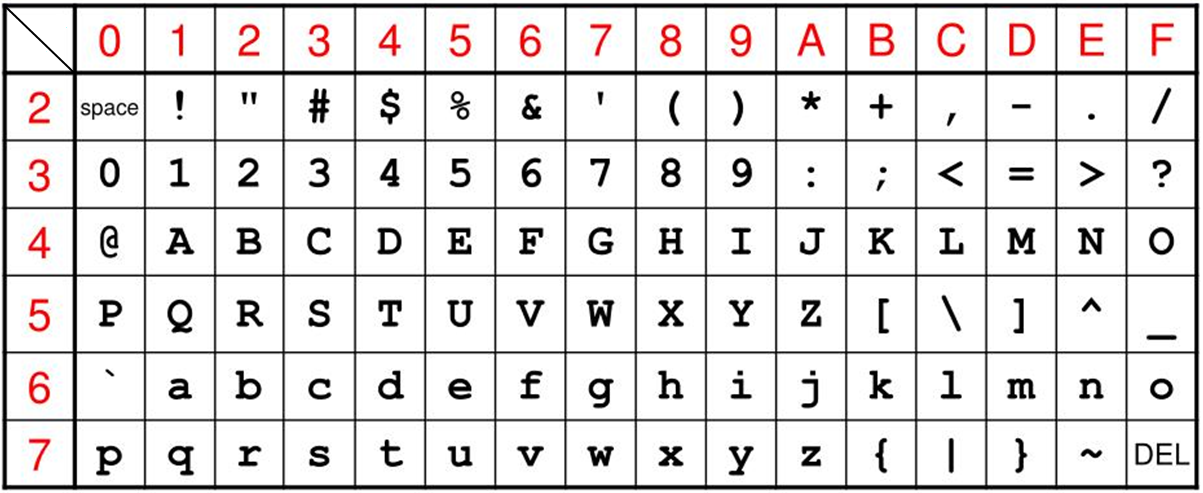
\includegraphics[width=\columnwidth]{img/ASCII.png}\\
    \textit{La table ASCII}
\end{center}
Le code ASCII se base sur un tableau contenant les caractères les plus utilisés en langue anglaise : les lettres de l'alphabet en majuscule (de A
à Z) et en minuscule (de a à z),
les dix chiffres arabes (de 0 à 9), des signes de ponctuation (point, virgule, point-virgule, deux points, points d'exclamation et
d'interrogation, apostrophe ou \textit{quote}, guillemet
ou \textit{double quotes}, parenthèses, crochets etc.), quelques symboles et certains caractères spéciaux invisibles (espace, retour-chariot,
tabulation, retour-arrière, etc.).\\

\begin{exercice}
    Combien y a -t-il de caractères dans ce catalogue ?\\
    Combien de bits sont nécessaires pour pouvoir représenter tous leurs numéros de code ?
\end{exercice}


Pour représenter ces symboles ASCII, les ordinateurs utilisaient des cases mémoires de un octet, mais ils réservaient toujours le huitième bit pour le contrôle de parité : c'est un procédé de sécurité pour
éviter les erreurs, qui étaient très fréquentes dans les premières mémoires électroniques.\\
\begin{methode}[ : contrôle d'erreur par parité]
    \begin{itemize}
        \item 	On dispose d'un mot de 7 bits, par exemple 111 0011
        \item 	On compte le nombre de bits à 1, il y en a 5.
        \item 	On rajoute le bit de poids fort à 1 pour qu'en tout, il y ait toujours \textit{un nombre pair} de bits à 1.\\
              On obtient \boxed{1}111 0011, ce bit de poids fort jouant le rôle de \textit{code correcteur}.
        \item 	Un autre exemple : 001 1110 est codé \boxed{0}001 1110.
    \end{itemize}
\end{methode}

\begin{exercice}[]
    Voici un message reçu à l'issue d'une transmission :
    \begin{center}
        \texttt{53 E1 6C F5 70}
    \end{center}
    Ces 6 octets sont censés représenter 6 caractères ASCII, codées sur 7 bits le 8\eme étant réservé au contrôle d'erreur par parité.
    \begin{enumerate}
        \item 	Décoder ces 6 octets en disant s'il y a des erreurs ou non.
        \item 	Quel était le message initial ?
    \end{enumerate}
\end{exercice}


\section{L'insuffisance de l'ASCII}

Pour coder les lettres accentuées, inutilisées en Anglais mais très fréquentes dans d'autres langues (notamment le Français), on a décidé
d'étendre
le codage des caractères au huitième bit (les erreurs-mémoire étant devenues plus rares et les méthodes de contrôle d'erreurs plus efficaces).\\


\begin{exercice}[]
    Combien de nouveaux symboles a-t-on pu coder en autorisant le huitième bit dans le codage ?
\end{exercice}


On a alors pu coder toutes ces lettres et ainsi que de nouveaux caractères typographiques utiles tels que différents tirets.\\


\section{Le problème}

Le fait d'utiliser un bit supplémentaire a bien entendu ouvert des possibilités mais malheureusement les caractères de toutes les langues ne
pouvaient être pris en charge
en même temps.\\
La norme ISO 8859–1 appelée aussi Latin-1 ou Europe occidentale est la première partie d'une norme plus complète appelée \textbf{ISO 8859} (qui
comprend 16 parties)
et qui permet de coder tous les caractères des langues européennes. Cette norme ISO 8859–1 permet de coder 191 caractères de l'alphabet latin qui
avaient à
l'époque été jugés essentiels dans l'écriture, mais omet quelques caractères fort utiles (ainsi, la ligature œ n'y figure pas).\\

Dans les pays occidentaux, cette norme est utilisée par de nombreux systèmes d'exploitation, dont Linux et Windows. Elle a donné lieu à quelques
extensions
et adaptations, dont \textbf{Windows-12527} (appelée \textbf{ANSI}) et ISO 8859-158 (qui prend en compte le symbole €\  créé après la norme
ISO 8859-1).
C'est une source de grande confusion pour les développeurs de programmes informatiques car un même caractère peut être codé différemment suivant
la norme utilisée .\\
Voici les tableaux décrivant deux encodages :

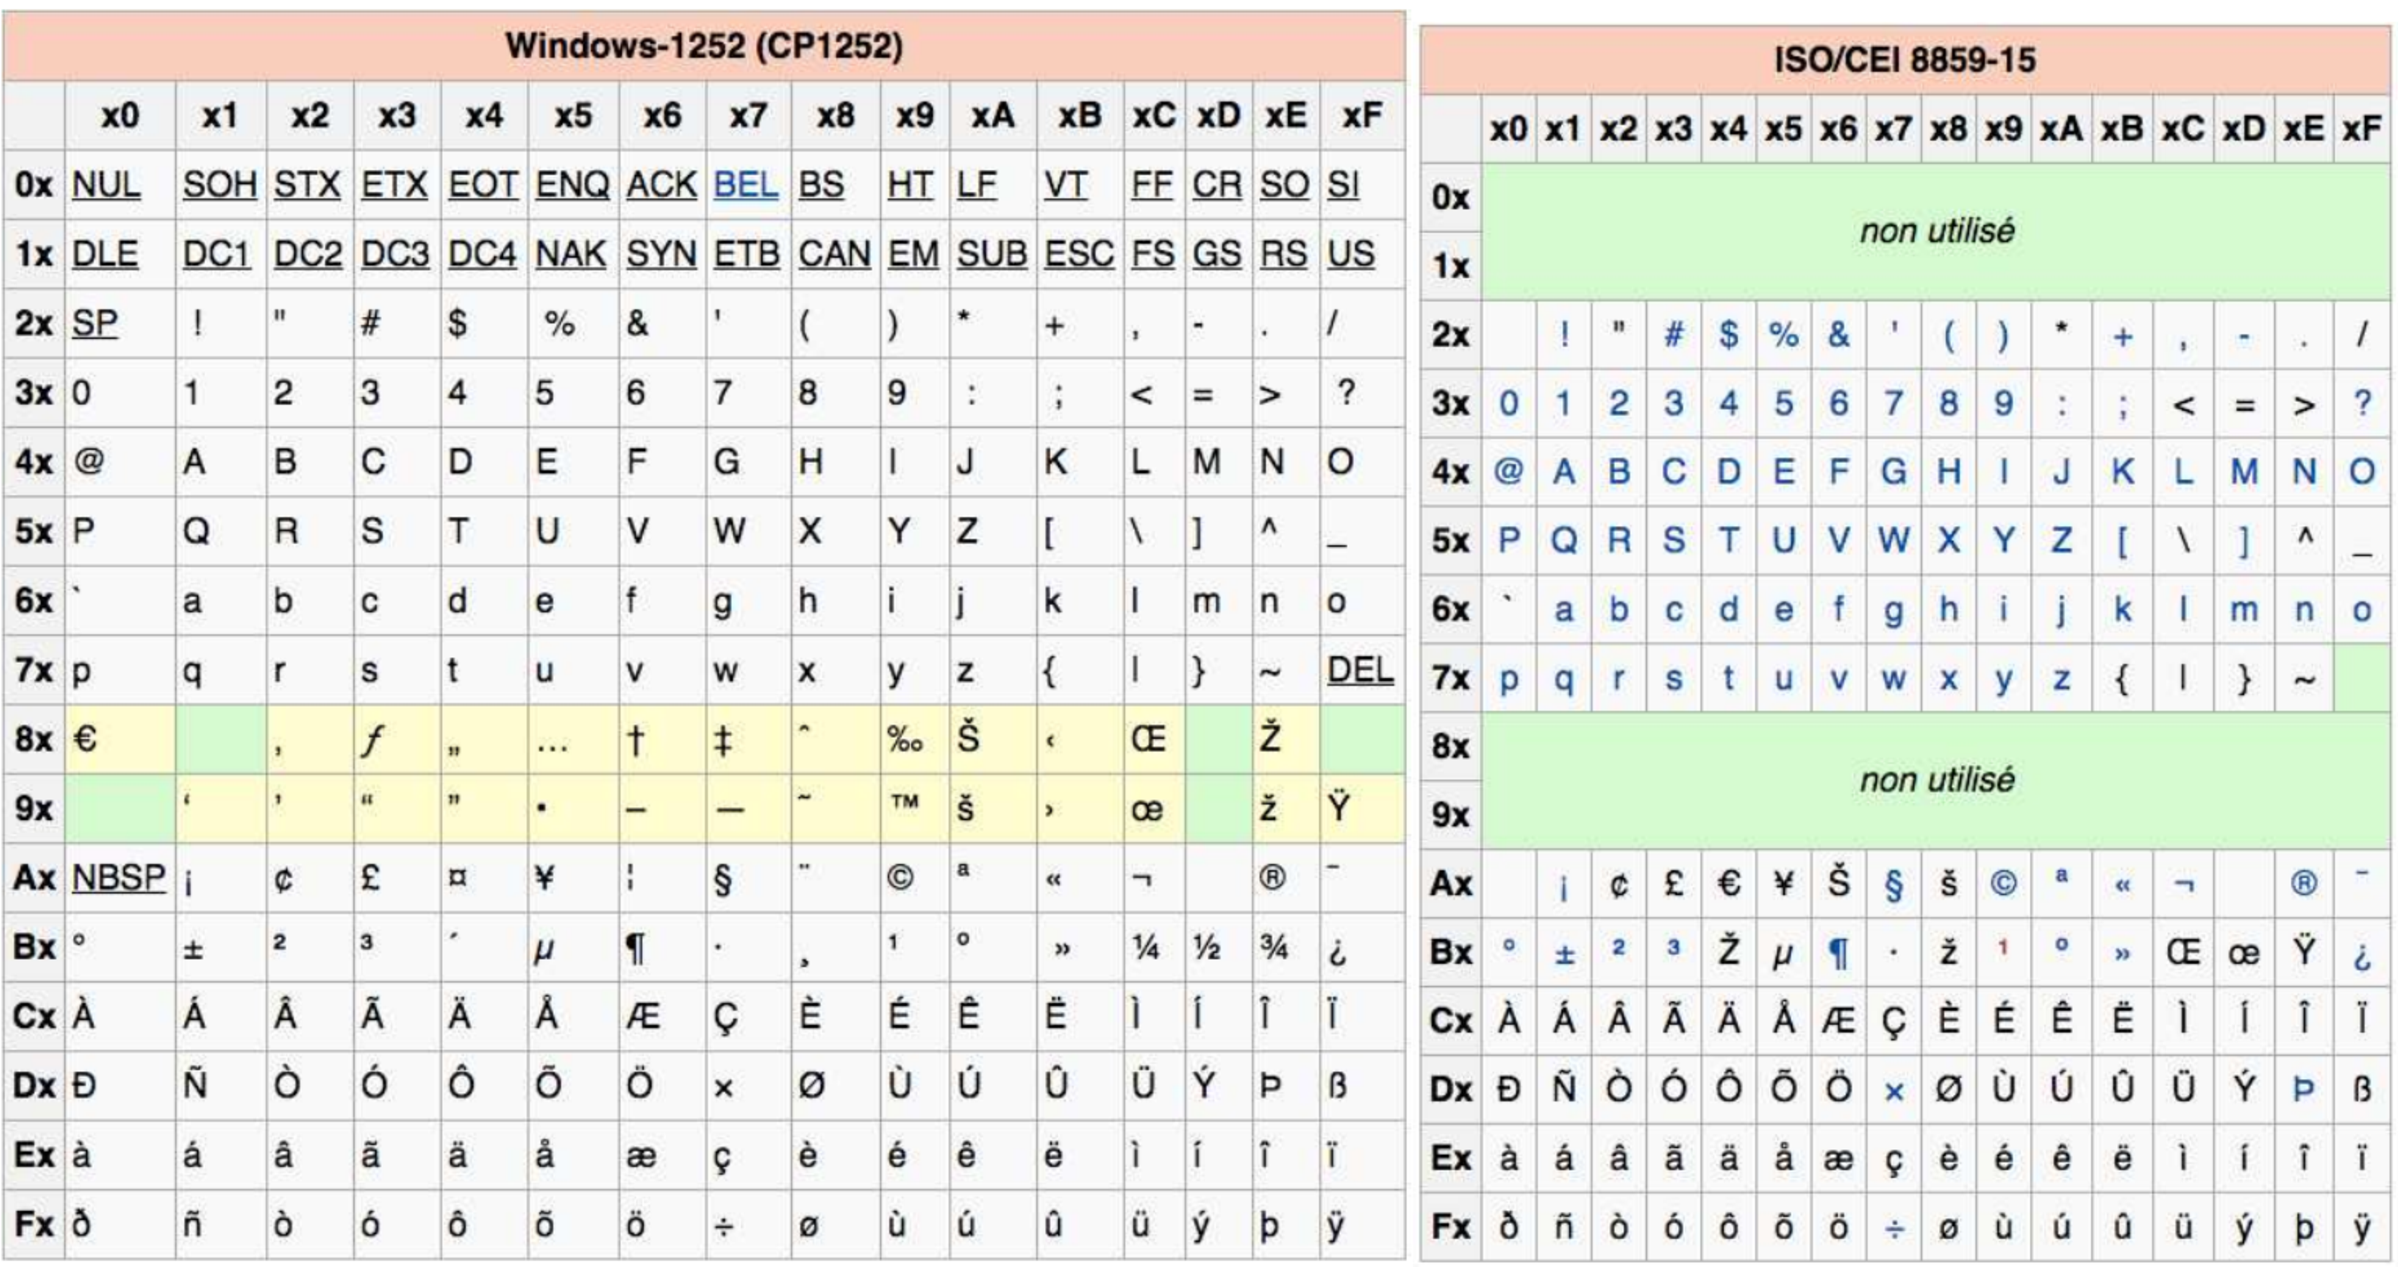
\includegraphics[width=\columnwidth]{img/W1252andISO}\\


\begin{exercice}[]
    Ces deux encodages sont-ils totalement compatibles ? Pourquoi ?
\end{exercice}

\section{La multiplicité des encodages}

Au fil du temps une multitude d'encodages sont apparus, multipliant les sources de confusion.\\
Voici pour l'exemple une partie des encodages que \textsc{Python} reconnaît :
\alternaterowcolors
\begin{center}
    {\tiny
        \begin{tabular}{|c|c|c|}
            \hline
            \rowcolor{UGLiOrange}{\boxfont\color{white}Encodage} & {\boxfont\color{white}Alias Python}                                                    & {\boxfont\color{white}Langues concernées}                           \\
            \hline
            ascii             & 646,us-ascii                                                             & English                                               \\\hline
            big5              & big5-tw, csbig5                                                          & Traditional Chinese                                   \\\hline
            cp424             & EBCDIC-CP-HE, IBM424                                                     & Hebrew                                                \\\hline
            cp437             & 437, IBM437                                                              & English                                               \\\hline
            cp500             & EBCDIC-CP-BE, EBCDIC-CP-CH, IBM500                                       & Western Europe                                        \\\hline
            cp720             &                                                                          & Arabic                                                \\\hline
            cp737             &                                                                          & Greek                                                 \\\hline
            cp856             &                                                                          & Hebrew                                                \\\hline
            cp857             & 857, IBM857                                                              & Turkish                                               \\\hline
            cp864             & IBM864                                                                   & Arabic                                                \\\hline
            cp874             &                                                                          & Thai                                                  \\\hline
            cp932             & 932, ms932, mskanji, ms-kanji                                            & Japanese                                              \\\hline
            cp1251            & windows-1251                                                             & Bulgarian, Byelorussian, Macedonian, Russian, Serbian \\\hline
            cp1258            & windows-1258                                                             & Vietnamese                                            \\\hline
            euc\_kr           & euckr, korean, ksc5601, ks\_c-5601, ks\_c-5601-1987, ksx1001, ks\_x-1001 & Korean                                                \\\hline
            gbk               & 936, cp936, ms936                                                        & Unified Chinese                                       \\\hline
            latin\_1          & iso-8859-1, iso8859-1, 8859, cp819, latin, latin1, L1                    & West Europe                                           \\\hline
            iso8859\_14       & iso-8859-14, latin8, L8                                                  & Celtic languages                                      \\\hline
            koi8\_r           &                                                                          & Russian                                               \\\hline
            utf\_8            & U8, UTF, utf8                                                            & all languages                                         \\\hline
        \end{tabular}}
\end{center}

\begin{exercice}[]
    Lequel de ces encodages semble le plus performant ?
\end{exercice}


\section{L'Unicode}

La globalisation des échanges culturels et économiques a mis l'accent sur le fait que les langues européennes coexistent avec de nombreuses
autres
langues aux alphabets spécifiques voire sans alphabet (le Japonais utilise entre autres un syllabaire, chaque symbole représentant une syllabe).
La
généralisation de l'utilisation d'Internet dans le monde a ainsi nécessité une prise en compte d'un
nombre beaucoup plus important de caractères (à titre d'exemple, le mandarin possède à lui tout seul plus de 5000 caractères !).\\
Une autre motivation pour cette
évolution résidait dans les possibles confusions dues au trop faible nombre de caractères pris en compte ; ainsi, les symboles monétaires des
différents
pays n'étaient pas tous représentés dans le système ISO 8859-1, de sorte que les ordres de paiement internationaux transmis par courrier
électronique
risquaient d'être mal compris. La norme Unicode a donc été créée pour permettre le codage de textes écrits quel que soit le système d'écriture
utilisé.\\

Dans le système UTF-8, on attribue à chaque caractère un nom, une position normative et un bref descriptif qui seront les mêmes quelle que soit
la plate-forme informatique
ou le logiciel utilisés.\\
Un consortium composé d'informaticiens, de chercheurs, de linguistes et de personnalités représentant les états ainsi que les entreprises
s'occupe d'unifier toutes les pratiques en un seul et même système : \textit{l'Unicode}.\\

\begin{definition}
    L'\textit{Unicode}  est  une table de correspondance Caractère-Code (Charset), et l'\textit{UTF-8} est l'encodage correspondant (Encoding) le
    plus répandu.
\end{definition}

De nos jours, par défaut, les navigateurs Internet utilisent le codage UTF-8 et les concepteurs de sites pensent de plus en plus à créer leurs
pages web
en prenant en compte cette même norme ; c'est pourquoi il y a de moins en moins de problèmes de compatibilité : l'UTF-8 est aujourd'hui
majoritairement utilisé pour les sites du web, comme le montre ce graphique.

\begin{center}
    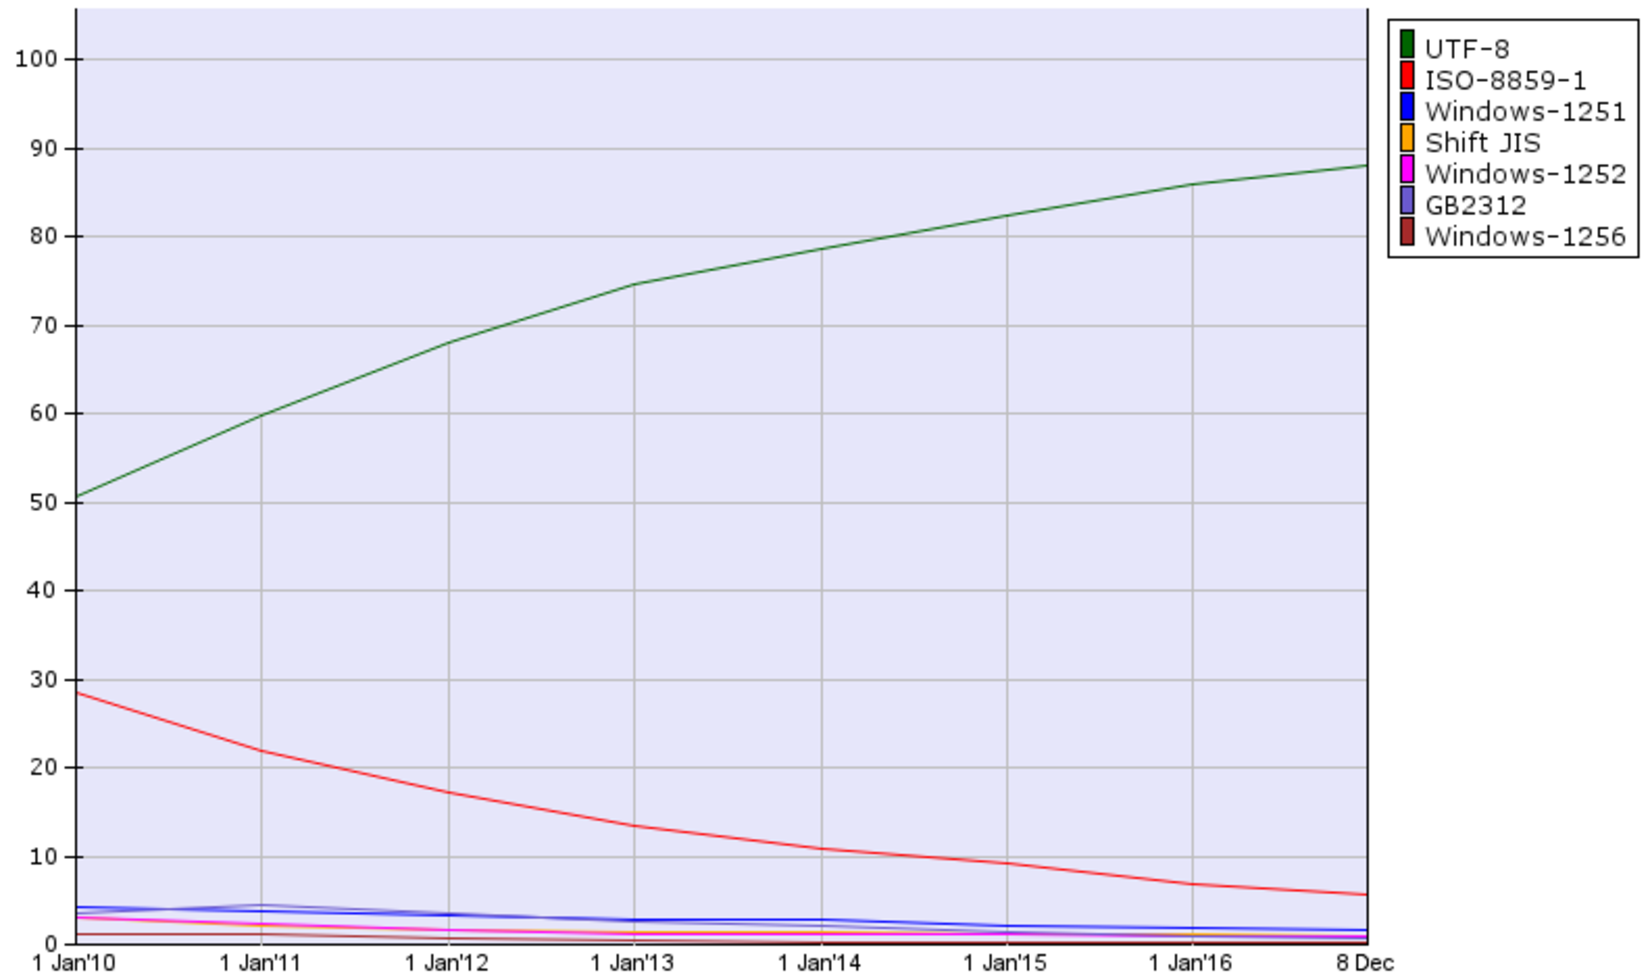
\includegraphics[width=10cm]{img/UTF8evol}
\end{center}

L'UTF-8 est également le codage le plus utilisé dans les systèmes GNU, Linux et compatibles pour gérer le plus simplement
possible des textes et leurs traductions dans tous les systèmes d'écritures et tous les alphabets du monde.\\

\section{L'UTF-8 côté technique}

La norme Unicode définit entre autres un ensemble (ou répertoire) de caractères. Chaque caractère est repéré dans cet ensemble par un index
entier aussi appelé « point de code ».\\
Par exemple le caractère « € » (euro) est le 8365$^{\text{ème}}$ caractère du répertoire Unicode, son index, ou point de code, est donc
8364
(on commence à compter à partir de 0).\\
Le répertoire Unicode peut contenir plus d'un million de caractères, ce qui est bien trop grand pour être codé par un seul octet (limité à des
valeurs entre 0 et 255).
La norme Unicode définit donc des méthodes standardisées pour coder et stocker cet index sous forme de séquence d'octets :
UTF-8 est la plus utilisée d'entre elles (il y a aussi des variantes comme UTF-16 et UTF-32).
En UTF-8, tout caractère est codé sur 1, 2, 3 ou 4 octets.\\
La principale caractéristique d'UTF-8 est qu'elle est \textit{rétro-compatible avec la norme ASCII}, c'est-à-dire que tout caractère ASCII se
code
en UTF-8 sous forme d'un unique octet, identique au code ASCII.\\
Par exemple « A » (A majuscule) a pour code ASCII 65 et se code en UTF-8 par l'octet 65, il en va de même pour tous les caractère ASCII.
Pour les autres, on procède comme ceci :
\begin{itemize}
    \item Chaque caractère est associé à son index Unicode.
    \item 	En général, cet index est exprimé en hexadécimal.
          Actuellement, presques toutes les valeurs de 0000 à FFFF, c'est-à-dire de 0 à 65535 sont
          attribuées à des \og alphabets \fg{} associés à des langues, des plus communes aux plus rares, et à divers symboles, tels que les
          symboles mathématiques.
          Au delà de FFFF on trouve des alphabets associés à des langues anciennes (cunéiformes, hiéroglyphes\ldots).
    \item  En fonction du nombre de bits nécessaires pour représenter en binaire  cet index, on utilise le codage suivant :\\

          \begin{center}
              {\scriptsize
                  \begin{tabular}{|c|c|c|}
                      \hline
                      \rowcolor{UGLiOrange}{\boxfont\color{white}Nombre de bits de l'index} & {\boxfont\color{white}Nombre d'octets pour coder en UTF-8} & {\boxfont\color{white}Schéma de codage}                                                           \\
                      \hline
                      de 0 à 7                  & 1                                   & 0xxx xxxx                                                                   \\
                      \hline
                      de 8 à 11                 & 2                                   & \textbf{110}x xxxx \textbf{10}xx xxxx                                       \\
                      \hline
                      de 12 à 16                & 3                                   & \textbf{1110} xxxx \textbf{10}xx xxxx \textbf{10}xx xxxx                    \\
                      \hline
                      de 17 à 21                & 4                                   & \textbf{1111 0}xxx \textbf{10}xx xxxx \textbf{10}xx xxxx \textbf{10}xx xxxx \\
                      \hline
                  \end{tabular} }
              \normalsize
          \end{center}
          \vspace{1em}
\end{itemize}
Par exemple le symbole €\  a un index Unicode qui vaut 8364.\\
\begin{itemize}
    \item 	8364 s'écrit 20AC en hexa, ce qui fait 10 0000 1010 1100 en binaire, soit 14 bits.\\
          On va donc utiliser 3 octets pour coder, conformément au schéma de codage.
    \item 	On commence par écrire le mot de 16 bits correspondant : \boxed{00}10 0000 1010 1100.\\
    \item 	On formate comme à la 3ème ligne du tableau : \\

          \textbf{1110} 0010 \textbf{10}00 0010 \textbf{10}10 1100\\

          Ce qui fait 3 octets : E2 82 AC en hexadécimal.\\

\end{itemize}


\begin{exercice}[]
    Si un ordinateur lit cet encodage UTF-8 du symbole €\  selon l'encodage ISO8859-15, qu'affichera-t-il ?\\

\end{exercice}


\section{Conclusion}

Même si l'encodage UTF-8 devient le standard international, certains développeurs, sites, ou applications en utilisent malgré tout encore
d'autres.\\

\begin{propriete}
    La notion de texte brut n'existe pas en informatique : lorsqu'un ordinateur lit un fichier texte il n'a \textit{a priori} aucun moyen de savoir
    quel est son encodage.
\end{propriete}

Beaucoup de documents indiquent donc en en tête leur format d'encodage : en HTML, on écrira dans l'en-tête d'une page:
\begin{html}
    \begin{minted}{html}
        <meta charset="utf8"/>
    \end{minted}
\end{html}

pour préciser qu'elle est encodée en UTF-8.\\
\section{Et Python dans tout ça ?}
En \textsc{Python}, on pourra aussi écrire : \mintinline{python}{# -*- coding: utf8 -*-} en première ligne de tout script pour signifier la même chose, \textit{et c\ae tera}.\\

\textsc{Python} gère très bien les encodages. On peut fabriquer un convertisseur très rapidement :

\begin{pyc}
    \begin{minted}{python}
fichier = open("nom_fichier", 'rt', encoding="utf8")
texte = fichier.read()
fichier.close()
    \end{minted}
\end{pyc}

Ceci permet de lire le contenu d'un fichier texte (d'où le \mintinline{python}{'rt'}, pour 'read text') d'un fichier texte encodé en UTF-8, et de le stocker dans la
variable \texttt{texte}, de type \mintinline{python}{str}.\\

\begin{pyc}
    \begin{minted}{python}
fichier = open("nom_fichier", 'wt', encoding="utf8")
fichier.write("Salut")
fichier.close()	
    \end{minted}
\end{pyc}

Permet d'écrire un fichier texte (d'où le \mintinline{python}{'wt'}, pour write text) en UTF-8.\\

\section{Exercices}
\begin{exercice}
    Analyser les deux fichiers \texttt{texte1(utf8).txt} et \texttt{texte1(utf8).txt} : ils sont tous les deux encodés en UTF-8.


    \begin{itemize}
        \item Ouvrir chaque fichier. Quelles sont les différences de contenu entre ces deux fichiers ?
        \item Faire un clic droit puis \texttt{Propriétés} comme ceci :\\

              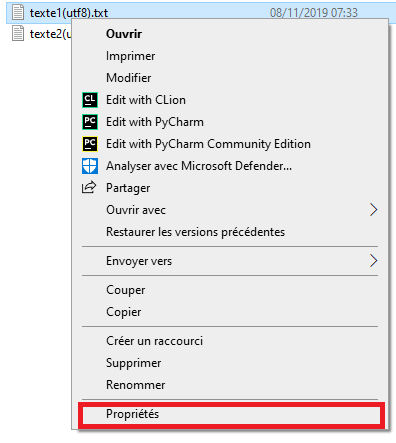
\includegraphics[width=7cm]{img/expli1}\\

              Quelles sont les tailles de ces deux fichiers ?\\
              Comment, dans le détail, la différence de taille s'explique-t-elle ?

    \end{itemize}
\end{exercice}

\begin{exercice} Nous allons examiner des problèmes d'encodage.
    \begin{itemize}
        \item Ouvrir le fichier \texttt{index1(utf8).html} avec un navigateur, puis le fichier \texttt{index2(utf8).html} avec un navigateur.\\
              Que remarquez-vous ?\\

        \item 	Ouvrir ce dernier fichier avec un éditeur de texte (comme le bloc-notes Windows).\\
              D'où vient le problème ? Proposer une correction.\\
              Expliquer en détail pourquoi à la place des \og é \fg{}, il y a des \og é \fg{} .\\

        \item 	Ouvrir le fichier \texttt{index3(ISO8859-15).html} avec un navigateur.\\
              D'où vient le problème ? Proposer une correction.\\
              Expliquer en détail pourquoi il y a des \og points d'interrogation dans des losanges noirs \fg{}.\\
    \end{itemize}
\end{exercice}

\begin{exercice}
    \'Ecrire un script qui corrige le problème de  \texttt{index3(ISO8859-15).html} en le convertissant en UTF-8 (utiliser les scripts \textsc{Python} fournis à la section précédente).

\end{exercice}

% \part{Programmation\\ avec Python}

% \chapter{Valeurs et types}
\section{Python, machine à évaluer}
\textsc{Python} est tout d'abord une machine à calculer, ou plutôt une machine à \textit{évaluer} : lorsque \textsc{Python} rencontre une \textit{expression}, c'est-à-dire une écriture qui produit une valeur, il commence par déterminer cette valeur.\\
Pour s'en rendre compte, il suffit d'écrire des expressions dans une \textit{console}.
\begin{pyc}
    \begin{minted}{python}
        >>> 5 - 3
        2
        
        >>> 11 / (1 + 2)
        3.6666666666666665

        >>> 30 / 15
        2.0
    \end{minted}
\end{pyc}
On se rend compte que les valeurs rencontrées ne sont pas présentées de la même manière : \mintinline{python}{5 - 3} a la valeur \mintinline{python}{2} alors que \mintinline{python}{30 / 15} a la valeur \mintinline{python}{2.0}.\\
Pour y voir plus clair, on peut appeler la fonction \mintinline{python}{type} qui 
\begin{itemize}
  \item en entrée prend une expression ;
  \item renvoie le \textit{type} de l'expression.
\end{itemize}
\begin{pyc}
  \begin{minted}{python}
    >>> type(2)
    <class int>

    >>> type(2.0)
    <class float>
  \end{minted}
\end{pyc}

Il y a donc au moins deux types de valeurs, le type \mintinline{python}{int} et le type \mintinline{python}{float}.\\
En fait il existe une multitude de types prédéfinis selon la nature de la valeur à représenter et nous allons les passer en revue.


\section{Le type int}
Il sert à représenter les \textit{entiers relatifs} (\textit{integer} signifie  « entier » en Anglais).\\
Le type \mintinline{python}{int} dispose des opérations \mintinline{python}{+} (addition), \mintinline{python}{-} (soustraction) et \mintinline{python}{*} (multiplication).

\begin{pys}\begin{minted}{python}
>>> 3 + 2
5

>>> 2 * 3
6

>>> 3 - 2 * 2
-1

>>> 10_000 # on utilise des _ pour séparer les chiffres
\end{minted}
\end{pys}

On dispose également de \textit{deux opérations très pratiques} : soient \mintinline{python}{a} et \mintinline{python}{b} deux \mintinline{python}{int}, et \mintinline{python}{b} non nul, alors on 
\begin{itemize}
  \item \mintinline{python}{a // b} est le \textit{quotient} de la \textit{division euclidienne} de \mintinline{python}{a} par \mintinline{python}{b} ;  
  \item \mintinline{python}|a % b| est le \textit{reste}.
\end{itemize}


\begin{pys}\begin{minted}{python}
>>> 64 // 10 # 64, c'est 6 * 10 + 4
6

>>> 64 % 10
4

>>> 22 // 7 # 22, c'est 3 * 7 + 1
3

>>> 22 % 7
1
\end{minted}
\end{pys}


On dispose de l'opération d'\textit{exponentiation} (opération puissance), notée \mintinline{python}{**}.\\
\textbf{Attention :} Cette opération peut produire un résultat \textit{non-entier}, de type \mintinline{python}{float} (voir partie suivante).

\begin{pys}\begin{minted}{python}
>>> 2 ** 3
8

>>> 10 ** 4
10000

>>> 2 ** (-1)
0.5
\end{minted}
\end{pys}

Pour finir, la \textit{division décimale} peut être effectuée sur des entiers, mais elle renvoie un résultat de type \mintinline{python}{float}.

\section{Le type float}
Il sert à représenter les \textit{nombres à virgule flottante} (\textit{to float} : flotter en Anglais). Ce sont (en gros) des nombres
décimaux.\ \textsc{Python} comprend et utilise la notation scientifique : \mintinline{python}{2.35e6} vaut $2,35\times 10^6$, c'est-à-dire 2 350 000.

\begin{pys}\begin{minted}{python}
>>>  2 / 7
0.2857142857142857 # c'est une valeur approchée

>>> 1 / 100_000
1e-05

>>> 1.2e-4
0.00012
\end{minted}
\end{pys}

On peut pratiquer sur les \mintinline{python}{float} toutes les opérations vues avec les \mintinline{python}{int}. Pour des fonctions plus compliquées telles le cosinus ou
l'exponentielle, on fait appel au module\footnote{Un module est un ensemble de \textit{fonctions} et/ou de \textit{constantes} que l'on peut importer.}
\mintinline{python}{math} :

\begin{pys}\begin{minted}{python}
>>> from math import *
>>> pi
3.141592653589793

>>> cos(pi / 3)
0.5000000000000001

>>> exp(2)
7.38905609893065

>>> log(2)
0.6931471805599453

>>> exp(log(2))
2.0
\end{minted}
\end{pys}

\mintinline{python}{exp} est la \textit{fonction exponentielle} et \mintinline{python}{log} la \textit{fonction logarithme népérien}\footnote{Voir le programme de mathématiques
    de terminale scientifique.} notée $\ln$ en France.



\section{Le type str}

Il sert à représenter les \textit{chaînes de caractères} (\mintinline{python}{str} est l'abréviation de \textit{string}, qui veut dire chaîne en anglais).
Lorsqu'on écrit une valeur de type \mintinline{python}{str}, on peut utiliser les symboles \mintinline{python}{'}, \mintinline{python}{"} ou même \mintinline{python}{'''} (suivant que la chaîne contient des apostrophes, ou des guillemets).

\begin{pys}\begin{minted}{python}
>>> 'Bonjour.'
'Bonjour'

>>> 'J'aime Python.'
SyntaxError

>>> "J'aime Python."
"J'aime Python."

>>> "Je n'aime pas qu'on m'appelle "geek"."
SyntaxError

>>> """Je n'aime pas qu'on m'appelle "geek"."""
'Je n\'aime pas qu\'on m\'appelle "geek".'
\end{minted}
\end{pys}
La dernière évaluation produit une valeur correcte. \textsc{Python} utilise simplement \mintinline{python}{\'} pour écrire les apostrophes qui sont à l'intérieur de la valeur.\\


Le symbole \mintinline{python}{+} sert à \textit{concaténer 2 chaînes}, c'est-à-dire à les mettre bout à bout.  

\begin{pys}\begin{minted}{python}
>>> 'Yes' + 'No'
'YesNo'

>>> 'No' + 'Yes'
'NoYes'
\end{minted}
\end{pys}

On peut même multiplier un \mintinline{python}{str} par un \mintinline{python}{int} :
\begin{pyc}
  \begin{minted}{python}
    >>> 3*'Aïe ! '
    'Aïe ! Aïe ! Aïe ! '
  \end{minted}
\end{pyc}
\textsc{Python} évalue \mintinline{python}{3*'Aïe !'} comme \mintinline{python}{'Aïe ! ' + 'Aïe ! ' + 'Aïe ! '}.


Voici deux types très utiles que nous étudierons en détail plus tard.

\section{Le type list}

Une valeur de type \mintinline{python}{list} est une... liste ordonnée de valeurs. Celles-ci peuvent être du même type ou non.

\begin{pyc}
  \begin{minted}{python}
    >>> [] # liste vide
    []

    >>> [1, 4, 5] # liste comportant 3 int
    [1, 4, 5]

    >>> [2.0, -4, 'Bonjour', 'Coucou']
    [2.0, -4, 'Bonjour', 'Coucou']
  \end{minted}
\end{pyc}

L'intérêt de ce type est de rassembler plusieurs valeurs au sein d'une seule, qui pourra ensuite être \textit{parcourue}.

\section{Le type dict}

Celui-ci sert à établir des \textit{association} du type \textit{clé : valeur}.

\begin{pyc}
    \begin{minted}{python}
      >>> {} # dictionnaire vide
      {}

      >>> {'France': 'Paris', 'Canada': 'Ottawa', 'Pays-Bas': 'La Haye'}
      {'France': 'Paris', 'Canada': 'Ottawa', 'Pays-Bas': 'La Haye'}
    \end{minted}
  \end{pyc}  

Tout comme le type \mintinline{python}{list}, ce type sert à \textit{structurer les données}. L'exemple précédent fait correspondre des capitales à des pays.



\section{Le type bool}
Il sert à représenter les \textit{valeurs booléennes}, valant \mintinline{python}{True} (vrai) ou
\mintinline{python}{False} (faux).

\begin{pys}\begin{minted}{python}
>>> False
False

>>> True
True
\end{minted}
\end{pys}

Cela peut paraître un peu pauvre, c'est trompeur : les \textit{expressions logiques} sont des écritures dont la valeur est un booléen. Lorsque \textsc{Python} les rencontre, il les évalue pour trouver soit \mintinline{python}{True} soit \mintinline{python}{False}.

\begin{pyc}
  \begin{minted}{python}
    >>> 3 >= 2 # évalue si 3 est supérieur ou égal à 2
    True
    
    >>> 3 + 5 == 2 # évalue si 3 + 5 vaut 2
    False

    >>> 1 in [3, 4, 1, 5] # évalue si 1 est un élément de la liste
    True
  \end{minted}
\end{pyc}

\begin{remarque}[]
  Pour \textit{tester} si deux valeurs sont égales, on utilise \mintinline{python}{==}  (et pas \mintinline{python}{=} ).
\end{remarque}

Ce type dispose d'\textit{opérations logiques} : \mintinline{python}{or} (ou), \mintinline{python}{and} (et) et \mintinline{python}{not} (non).

\begin{pyc}\begin{minted}{python}
>>> True and False # vrai que si les 2 sont vrais
False

>>> True or False # faux que si les 2 sont faux
True

>>> not (3 < 1) # contraire
True

>>> (2 < 1) or (3 >= 0)
True
\end{minted}
\end{pyc}
% \chapter{Variables et affectations}

\section{Le symbole =}

En mathématiques, le symbole $=$ a plusieurs significations
\begin{itemize}
	\item dans $2+2=4$, on peut comprendre $=$ comme un opérateur d'évaluation : $2+2$, cela « donne » $4$ ;
	\item dans $\mathcal{P}=2\times(\ell+L)$, on peut considérer que $=$ sert à définir ce qu'est le périmètre d'un rectangle de dimensions $\ell$ et $L$ ; 
	\item dans $3x + 2 = 4x +5$, le $=$ sert à convenir que les 2 membres ont la même valeur et on cherche s'il existe un ou des nombres $x$ qui satisfont l'égalité (appelée équation) ;
	\item \textit{et cætera}. 
\end{itemize}

En \textsc{Python}, le symbole \mintinline{python}{=}  n'a qu'un seul sens : il sert à l'\textit{affectation}.

\section{L'affectation}
Il s'agit de « stocker » une valeur dans un endroit de la mémoire auquel \textsc{Python} donne un nom\footnote{En réalité c'est plus compliqué mais cela ne nous intéresse pas.}. Voici un exemple d'affectation : 
\begin{center}\Large
\mintinline{python}{a = 2}
\end{center}\
\begin{itemize}
	\item   \mintinline{python}{2} est une \textit{valeur} de type \mintinline{python}{int} ;
	\item   la \textit{variable} \mintinline{python}{a} est créée ;\
	\item   \mintinline{python}{a} est « attachée » à la valeur \mintinline{python}{2} ;
	\item   par extension \mintinline{python}{a} est également de type \mintinline{python}{int}.
\end{itemize}
Au cours d'un programme la valeur associée à une variable peut change\ldots D'où le nom de \textit{variable}.\\


\begin{definition}[ : affectation]
Lors d'une affectation
\begin{itemize}
	\item d'abord \textsc{Python} évalue ce qu'il y a à droite du symbole \mintinline{python}{=} ;
	\item ensuite il affecte cette valeur à la variable qui figure à gauche du symbole \mintinline{python}{=} ;
	\item si la variable n'existe pas déjà, elle est créée automatiquement ;
	\item le type de la variable, c'est le type de la valeur qu'on lui affecte. 
\end{itemize}
\end{definition}
Que fait le programme suivant ?

\begin{pyc}
\begin{minted}{python}
x = 0
x = x + 1
print(x)    
\end{minted}
\end{pyc}

\begin{itemize}
	\item il crée une variable \mintinline{python}{x} de type \mintinline{python}{int} valant \mintinline{python}{0} ;
	\item il évalue \mintinline{python}{x + 1}, trouve \mintinline{python}{1} et affecte cette valeur à \mintinline{python}{x} ;
	\item évalue \mintinline{python}{x}, trouve 1 et donc affiche \mintinline{python}{1}.
\end{itemize}

\begin{aretenir}
En mathématiques, $x = x + 1$ est une équation sans solution.\\

En \textsc{Python}, l'instruction \mintinline{python}{x = x + 1} sert à augmenter la valeur de \mintinline{python}{x} de 1 (on dit aussi \textit{incrémenter}).
\end{aretenir}

\subsection{Affectations multiples}
\textsc{Python} permet d'affecter plusieurs valeurs à plusieurs variables en même temps.

\begin{pys}\begin{minted}{python}
>>> a, b= 10, 2
>>> a
10

>>> b
2

>>> a, b = b, a # permet d'échanger a et b
>>> a
2

>>> b
10

\end{minted}
\end{pys}

\subsection{Notation condensée}
On est souvent amené à écrire des instructions telles que  \mintinline{python}{a = a + 1} ou \mintinline{python}{b = b / 2}. Cela peut être lourd quand les variables ne s'appellent
pas \mintinline{python}{a} ou \mintinline{python}{b} mais \mintinline{python}{rayon_sphere} ou \mintinline{python}{largeur_niveau}. On peut utiliser les notation suivantes :
\begin{pys}\begin{minted}{python}
>>> rayon_sphere = 3.4
>>> rayon_sphere /= 2
>>> rayon_sphere
1.7

>>> largeur_niveau = 19
>>> largeur_niveau += 1
>>> largeur_niveau
20
\end{minted}
\end{pys}

On dispose également de \mintinline{python}{*=}, \mintinline{python}{//=}, \mintinline{python}|%=|, \mintinline{python}{-=} et \mintinline{python}{**=}.

% % IO
% %!TEX root = cours.tex
\chapter{Tests et conditions}
\introduction{Ceci n'est pas un test !}
\section{Des outils pour comparer}

Ce sont les \textit{opérateurs de comparaison} :\\

{\small
\alternaterowcolors
\begin{tabular}{CCC}
	\rowcolor{lightgray}
	\rowcolor{UGLiOrange}{\boxfont\color{white} Opérateur} & {\boxfont\color{white} Signification} & {\boxfont\color{white} Remarques}                                                                     \\

	\mintinline{python}{<}                                       & strictement inférieur                 & Ordre usuel sur \mintinline{python}{int} et \mintinline{python}{float}, lexicographique sur \mintinline{python}{str}... \\

	\mintinline{python}{<=}                                      & inférieur ou égal                     & Idem                                                                                                  \\

	\mintinline{python}{>}                                       & strictement supérieur                 & Idem                                                                                                  \\

	\mintinline{python}{>=}                                      & supérieur ou égal                     & Idem                                                                                                  \\

	\mintinline{python}{==}                                      & égal                                  & \og avoir même valeur\fg\  \textit{Attention :} deux signes =                                         \\

	\mintinline{python}{!=}                                      & différent                             &                                                                                                       \\

	\mintinline{python}{is}                                      & identique                             & être le même objet                                                                                    \\

	\mintinline{python}{is not}                                  & non identique                         &                                                                                                       \\

	\mintinline{python}{in}                                      & appartient à                          & avec \mintinline{python}{str}, \mintinline{python}{list} et \mintinline{python}{dict}                                   \\

	\mintinline{python}{not in}                                  & n'appartient pas à                    & avec \mintinline{python}{str} et \mintinline{python}{list} et \mintinline{python}{dict}                                 \\
\end{tabular}
}\normalsize

\begin{pys}
	\begin{minted}{python}
>>> a = 2
>>> a == 2
>>> a == 3
>>> a == 2.0
>>> a is 2.0
>>> a != 100
>>> a > 2
>>> a >= 2
    \end{minted}
\end{pys}

\begin{pys}
	\begin{minted}{python}
>>> a = 'Alice'
>>> b = 'Bob'
>>> a < b
>>> 'e' in a
>>> 'e' in b
>>> liste = [1,10,100]
>>> 2 in liste
    \end{minted}
\end{pys}

Ces opérateurs permettent de réaliser des tests basiques. Pour des tests plus évolués on utilisera des \og mots de liaison \fg{} logiques.

\section{Les connecteurs logiques}

\begin{itemize}
	\item   \mintinline{python}{and} permet de vérifier que 2 conditions sont \textit{vérifiées simultanément}.
	\item   \mintinline{python}{or} permet de vérifier qu'\textit{au moins une} des deux conditions est vérifiée.
	\item   \mintinline{python}{not} est un opérateur de \textit{négation} très utile quand on veut par exemple vérifier qu'une condition est fausse.
\end{itemize}
Voici les tables de vérité des deux premiers connecteurs :

\begin{center}
	\begin{tabular}{|c|c|c|}
		\hline
		\mintinline{python}{and} & \textit{True}        & \textit{False}       \\
		\hline
		\textit{True}      & \mintinline{python}{True}  & \mintinline{python}{False} \\
		\hline
		\textit{False}     & \mintinline{python}{False} & \mintinline{python}{False} \\
		\hline
	\end{tabular}\hspace{2em}
	\begin{tabular}{|c|c|c|}
		\hline
		\mintinline{python}{or} & \textit{True}       & \textit{False}       \\
		\hline
		\textit{True}     & \mintinline{python}{True} & \mintinline{python}{True}  \\
		\hline
		\textit{False}    & \mintinline{python}{True} & \mintinline{python}{False} \\
		\hline
	\end{tabular}
\end{center}
À ceci on peut ajouter que \mintinline{python}{not True} vaut \mintinline{python}{False} et vice-versa.

\begin{pys}
	\begin{minted}{python}
>>> True and False
>>> True or False
>>> not True
    \end{minted}
\end{pys}

\begin{pys}
	\begin{minted}{python}
>>> resultats = 12.8
>>> mention_bien = resultats >= 14 and resultats < 16
>>> print(mention_bien)
    \end{minted}
\end{pys}

\section{if, else et elif}
Voici le schéma de fonctionnement d'un test \mintinline{python}{if} :
\begin{center}
	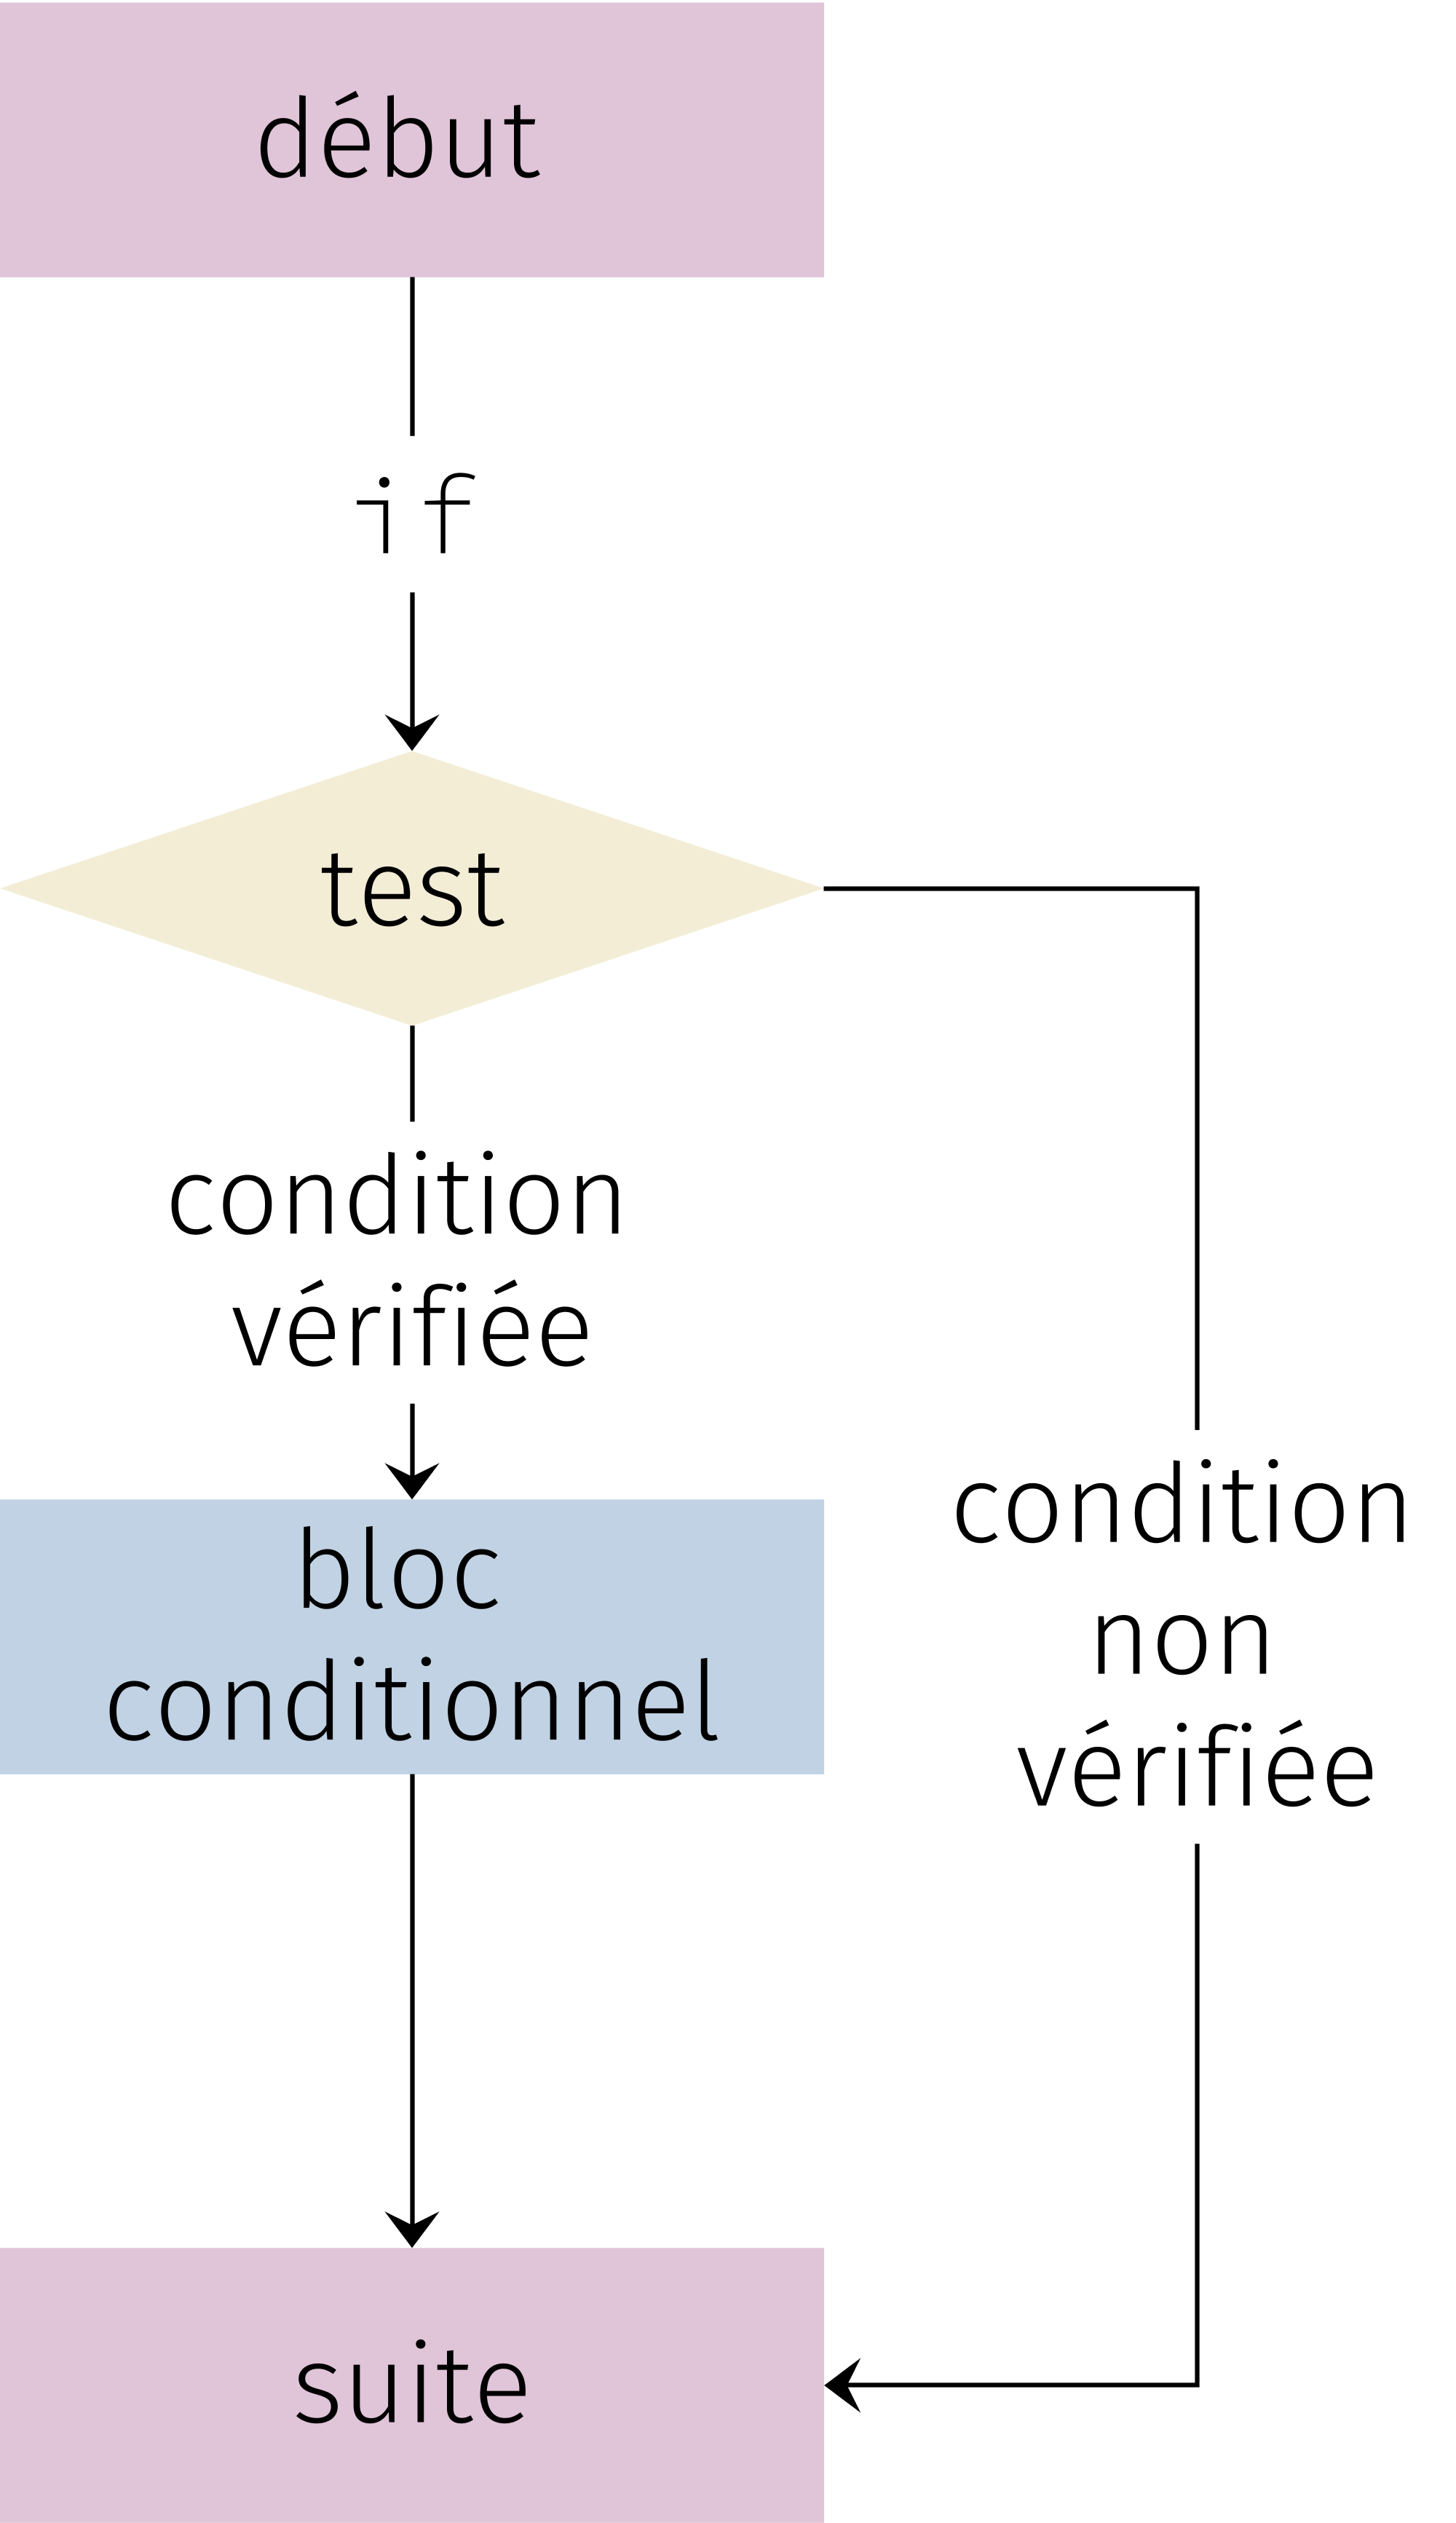
\includegraphics[height=10cm]{ch-conditions/img/if}
\end{center}

\textbf{Attention :} Un bloc conditionnel doit être \textit{tabulé} par rapport à la ligne précédente : il n'y a ni \mintinline{python}{DébutSi}  ni \mintinline{python}{FinSi}
en \textsc{Python}, ce sont les tabulations qui délimitent les blocs.

\begin{pyc}
	\begin{minted}{python}
phrase ='Je vous trouve très joli'
reponse = input('Etes vous une femme ?(O/N) : ')
if reponse == 'O':
    phrase += 'e'
phrase +='.'
print(phrase)
\end{minted}
\end{pyc}

Voici le schéma de fonctionnement d'un test \mintinline{python}{if...else} :
\begin{center}
	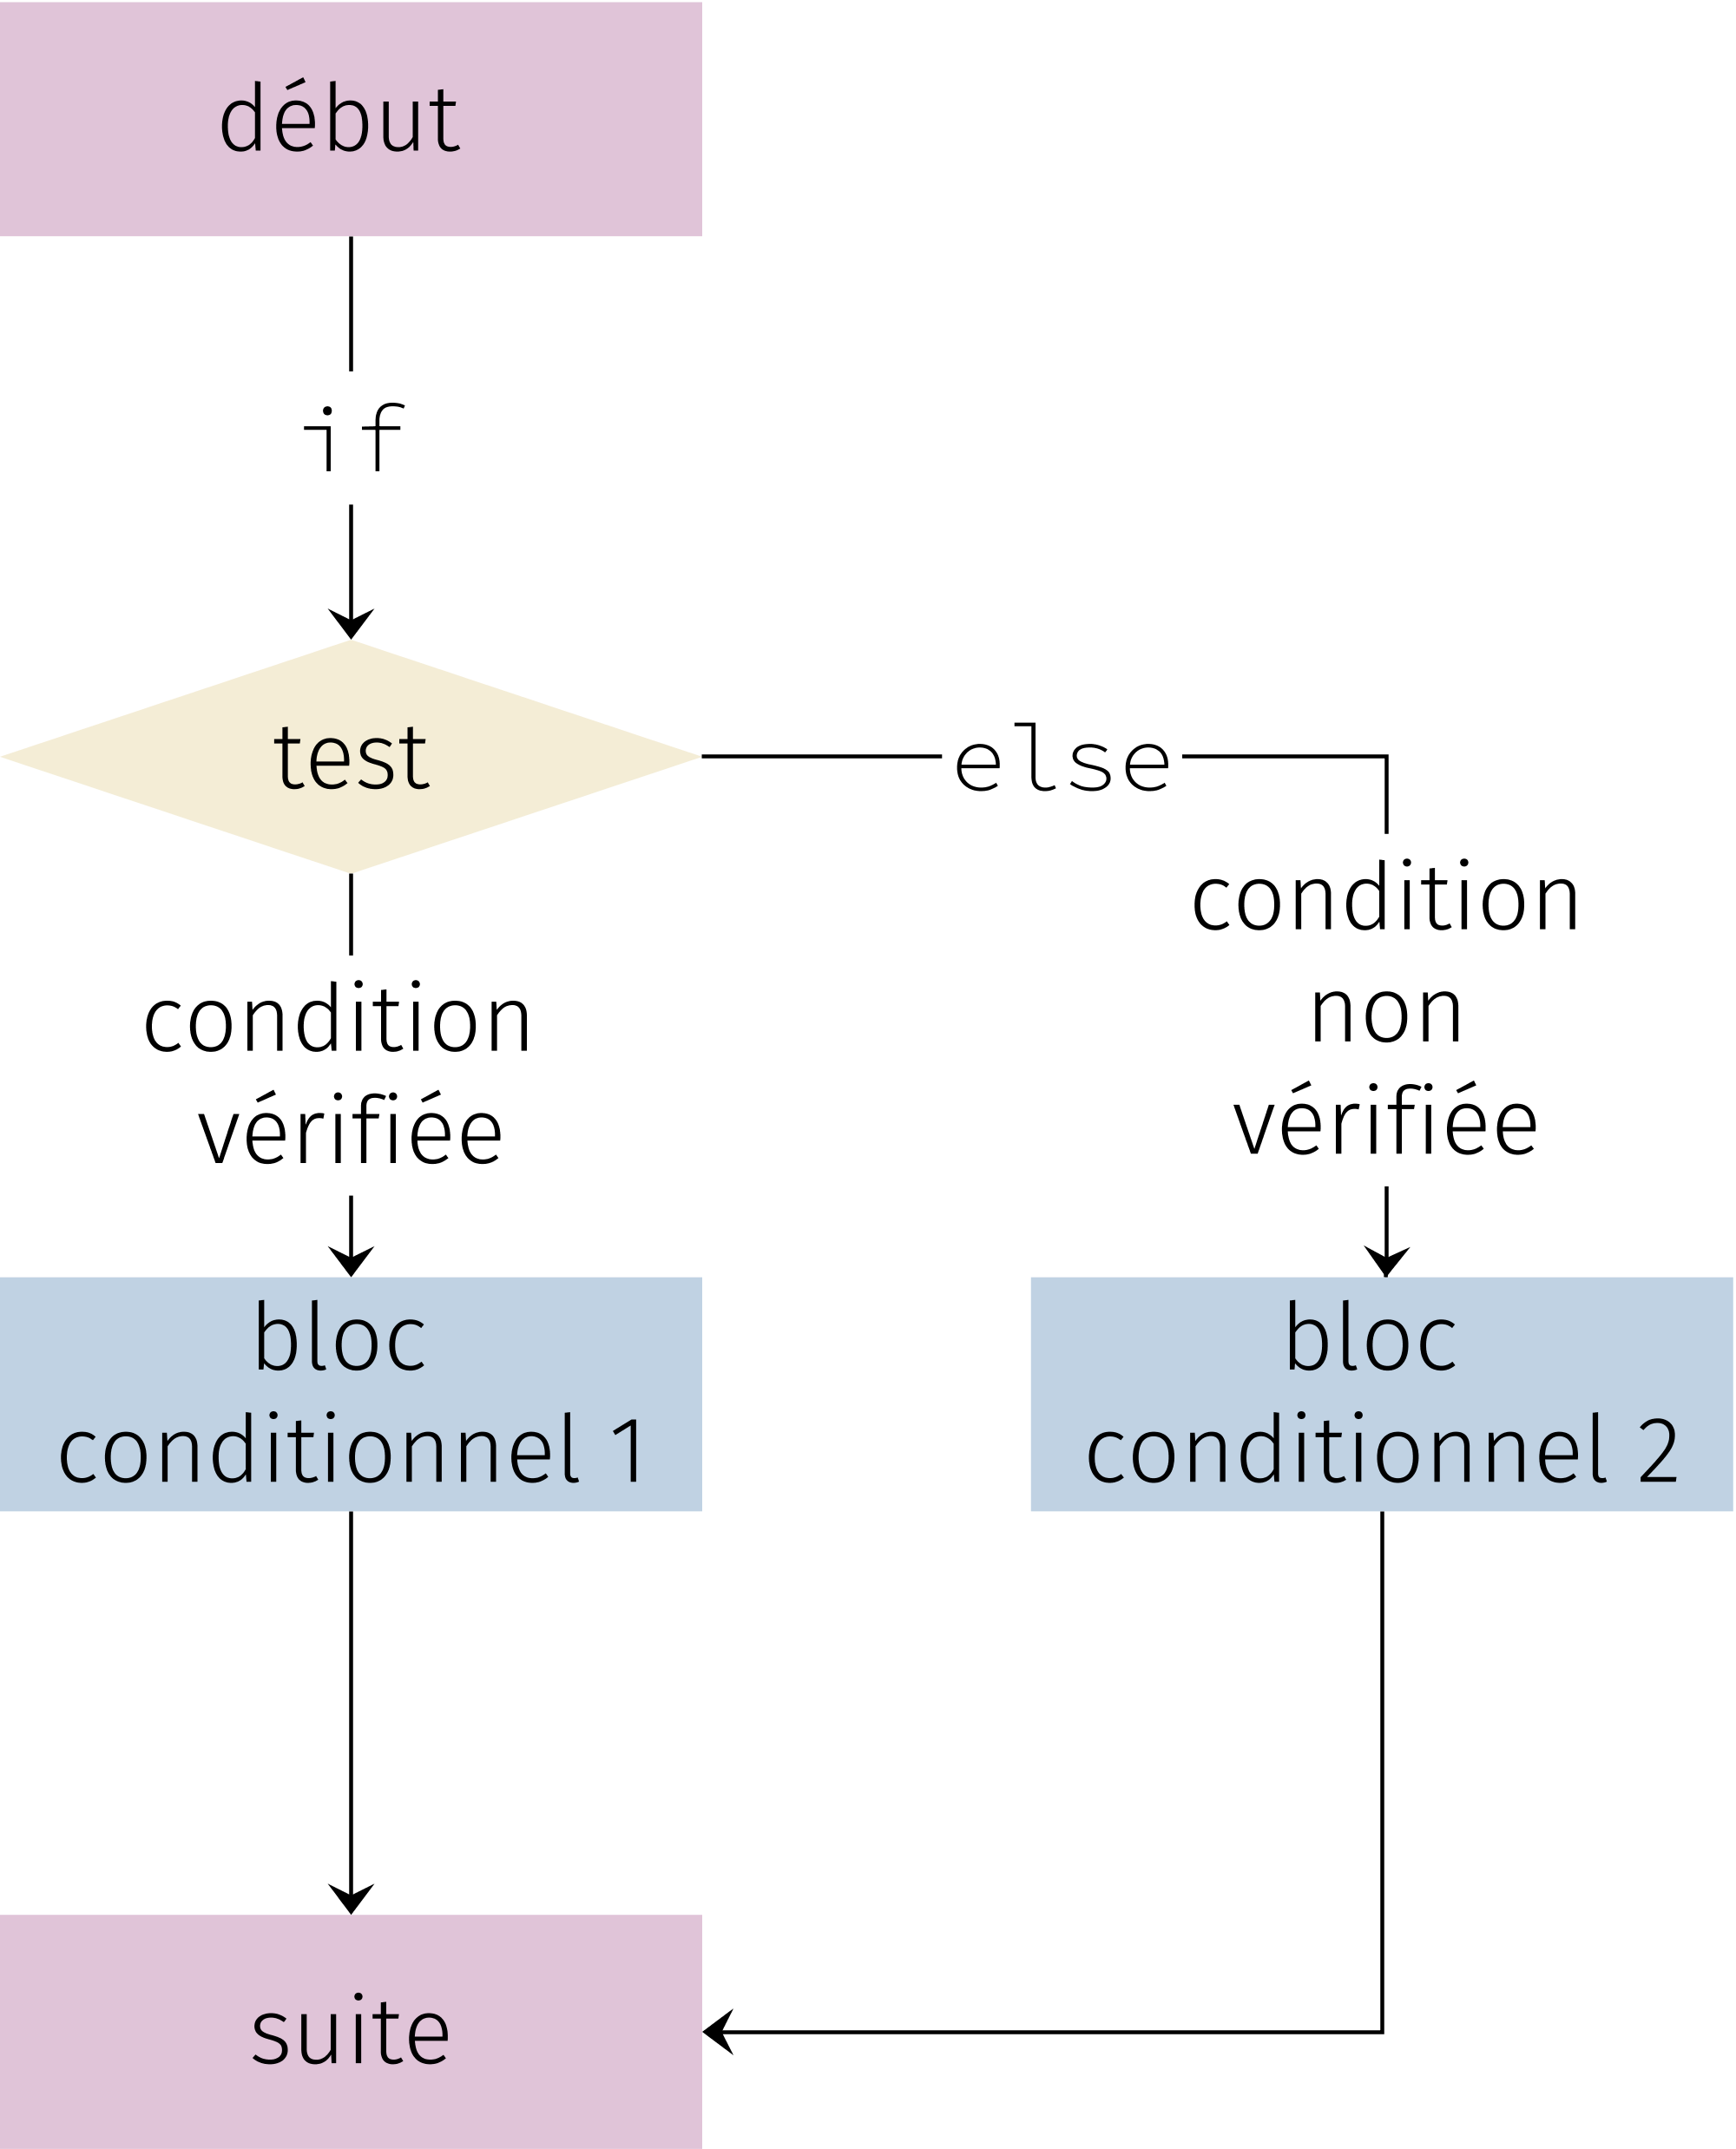
\includegraphics[height=10cm]{ch-conditions/img/ifelse}
\end{center}

\begin{pyc}
	\begin{minted}{python}
print('Bonjour')
age = int(input('Entrez votre age : '))
if age >= 18:
    print('Vous etes majeur')
else:
    print('Vous etes mineur.')
print('Au revoir.')
\end{minted}
\end{pyc}

Voici un exemple de fonctionnement d'un test \mintinline{python}{if...elif...} :
\begin{pyc}
	\begin{minted}{python}
print('Bonjour')
prenom = input('Entrez un prénom : ')
if prenom == 'Robert':
    print("Robert, c'est le prénom de mon grand-père.")
elif prenom == 'Raoul':
    print("Mon oncle s'appelle Raoul.")
elif prenom == 'Médor':
    print("Médor, comme mon chien !")
else:
    print("Connais pas")
print('Au revoir.')
\end{minted}
\end{pyc}
Et voici un schéma décrivant son fonctionnement :
\begin{center}
	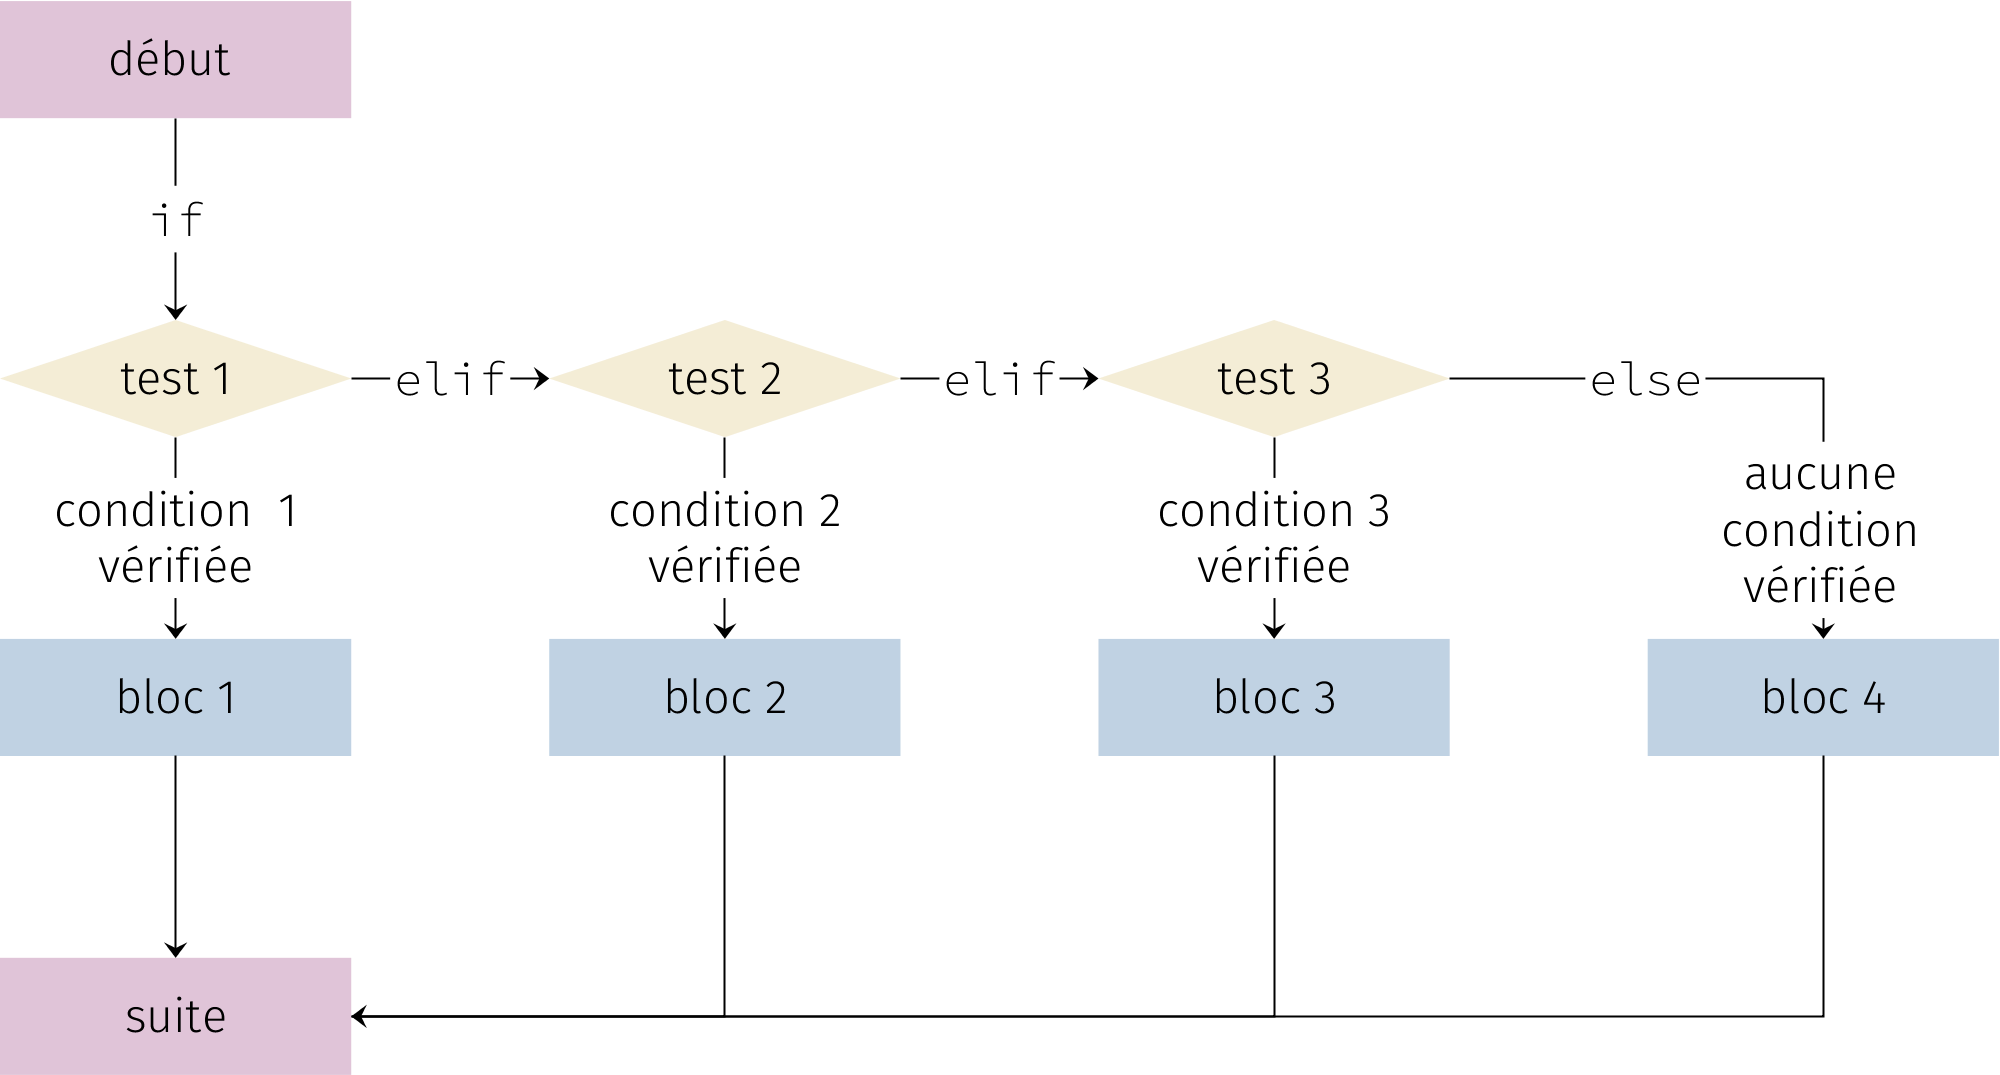
\includegraphics[width=\linewidth]{ch-conditions/img/ifelifelse}
\end{center}



On peut bien sûr inclure autant de \mintinline{python}{elif} que nécessaire.

\section{Exercices}

%----------------------------------------------------------------------
\begin{exercice}
	\'Ecrire un script qui demande son âge à l'utilisateur puis qui affiche \mintinline{python}{'Bravo pour votre longévité.'} si celui-ci est supérieur à 90.
\end{exercice}

\begin{exercice}[]
	\'Ecrire un script qui demande un nombre à l'utilisateur puis affiche si ce nombre est pair ou impair.
\end{exercice}
%----------------------------------------------------------------------
\begin{exercice}
	\'Ecrire un script qui demande l'âge d'un enfant à l'utilisateur puis qui l'informe ensuite de sa catégorie :
	\begin{itemize}
		\item   trop petit avant 6 ans;
		\item   poussin de 6 à 7 ans inclus;
		\item   pupille de 8 à 9 ans inclus;
		\item   minime de 10 à 11 ans inclus;
		\item   cadet à 12 ans et plus;
	\end{itemize}
\end{exercice}
%----------------------------------------------------------------------

\begin{exercice}
	\'Ecrire un script qui demande une note sur 20 à l'utilisateur puis vérifie qu'elle est bien comprise entre 0 et 20. Si c'est le cas rien ne se produit mais sinon le programme devra afficher un message tel que \mintinline{python}{'Note non valide.'}.
\end{exercice}

\begin{exercice}
	\'Ecrire un script qui demande un nombre à l'utilisateur puis affiche s'il est divisible par 5, par 7 par aucun ou par les deux de ces deux nombres.
\end{exercice}
%----------------------------------------------------------------------
\begin{exercice}
	En reprenant l'exercice du chapitre 1 sur les numéros de sécurité sociale, écrire un script qui demande à un utilisateur son numéro de sécurité sociale, puis qui vérifie si la clé est valide ou non.
\end{exercice}


%----------------------------------------------------------------------
\begin{exercice}
	\'Ecrire un script qui résout dans $\R$ l'équation du second degré $ax^2+bx+c=0$.\\
	On commencera par \mintinline{python}{from math import sqrt} pour utiliser la fonction \mintinline{python}{sqrt}, qui calcule la racine carrée d'un \mintinline{python}{float}.

	On rappelle que lorsqu'on considère une équation du type $ax^2+bx+c=0$
	\begin{itemize}
		\item   si $a=0$ ce n'est pas une équation de seconde degré;
		\item   sinon on calcule $\Delta = b^2-4ac$ et
		      \begin{itemize}
			      \item   Si $\Delta<0$ l'équation n'a pas de solutions dans $\R$;
			      \item   Si $\Delta=0$ l'équation admet pour unique solution $\dfrac{-b}{2a}$;
			      \item   Si $\Delta>0$ l'équation admet 2 solutions : $\dfrac{-b-\sqrt{\Delta}}{2a}$ et $\dfrac{-b+\sqrt{\Delta}}{2a}$.
		      \end{itemize}
	\end{itemize}
	Pour vérifier que le script fonctionne bien on pourra tester les équations suivantes :
	\begin{itemize}
		\item   $2x^2+x+7=0$ (pas de solution dans $\R$);
		\item   $9x^2-6x+1=0$ (une seule solution qui est $\dfrac{1}{3}$);
		\item   $x^2-3x+2$ (deux solutions qui sont 1 et 2).
	\end{itemize}
\end{exercice}

%----------------------------------------------------------------------
\begin{exercice}
	L'opérateur \mintinline{python}{nand} est défini de la manière suivante : si \mintinline{python}{A} et \mintinline{python}{B} sont deux booléens alors
	\begin{center}
		\mintinline{python}{A nand B} vaut \mintinline{python}{not (A and B)}
	\end{center}
	Construire la table de vérité de \mintinline{python}{nand} en complétant :
	\begin{center}

		\begin{tabular}{|c|c|c|c|}
			\hline
			\rowcolor{UGLiOrange}{\boxfont\color{white} A} & {\boxfont\color{white} B} & {\boxfont\color{white} A and B} & {\boxfont\color{white} not (A and B)} \\
			\hline
			\mintinline{python}{False}                           & \mintinline{python}{False}      &                                 &                                       \\
			\hline
			\mintinline{python}{False}                           & \mintinline{python}{True}       &                                 &                                       \\
			\hline
			\mintinline{python}{True}                            & \mintinline{python}{False}      &                                 &                                       \\
			\hline
			\mintinline{python}{True}                            & \mintinline{python}{True}       &                                 &                                       \\
			\hline
		\end{tabular}
	\end{center}
\end{exercice}



%  \chapter{Boucles}
\introduction{Tant que tu n'y arrives pas recommence.}
On s'intéresse dans ce chapitre aux \textit{structures itératives}, plus communément appelée \textit{boucles}.\\


\section{La boucle while}

Voici son schéma de fonctionnement :
\begin{center}
    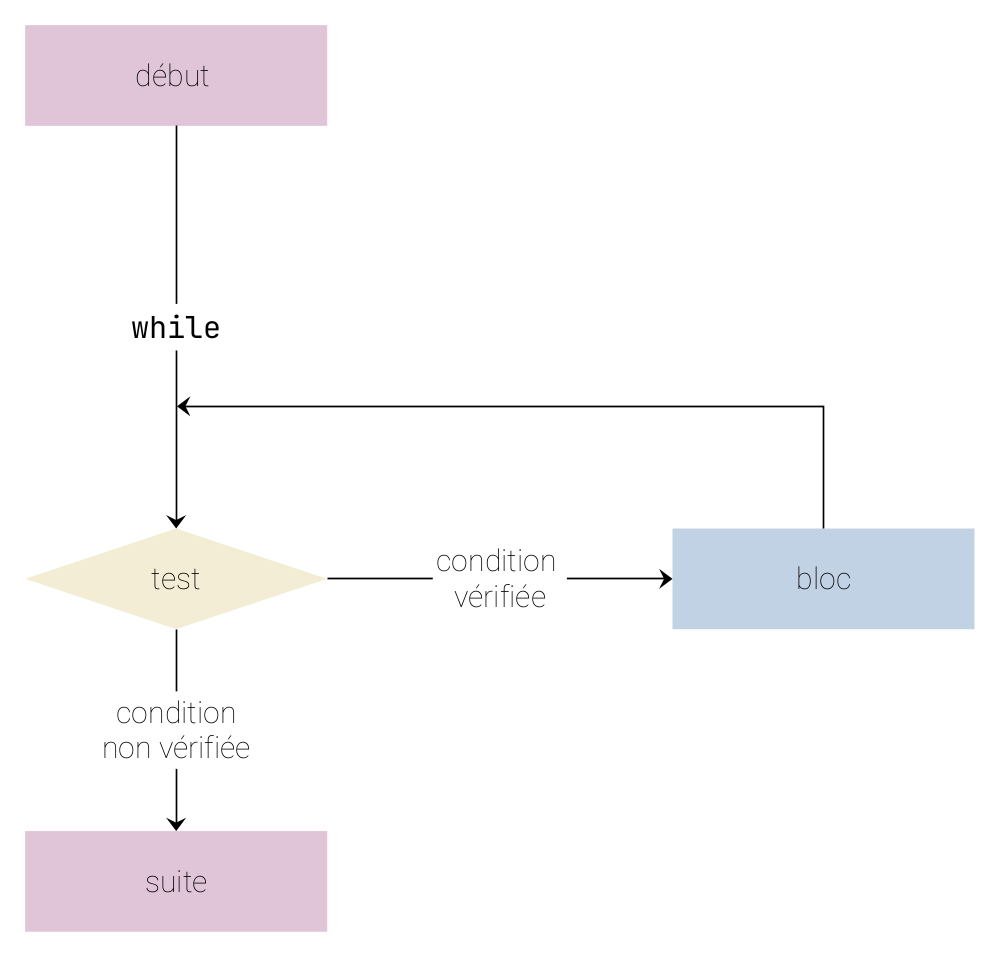
\includegraphics[height=7.5cm]{ch-boucles/img/while.png}
\end{center}

La boucle \mintinline{python}{while} exécute un bloc d'instructions conditionnel \textit{tant que} une condition est vérifiée.\\
Dès que la condition n'est plus vérifiée, le bloc conditionnel n'est plus exécuté.

\begin{pys}
\begin{minted}{python}
reponse=''
print('Bonjour !')
while reponse !='n':
    reponse = input('Voulez-vous continuer ? (o/n) : ')
print('Au revoir.')
\end{minted}
\end{pys}
La boucle \mintinline{python}{while} doit être utilisée avec soin : si la condition est toujours vérifiée, le programme ne s'arrêtera pas :

\begin{pyc}
\begin{minted}{python}
while True:
    print('Au secours !')
\end{minted}
\end{pyc}
Voici un exemple typique d'utilisation de la boucle \mintinline{python}{while} : \\

On place un capital de 2000 euros sur un compte à intérêts annuels de 2\%. On aimerait savoir au bout de combien de temps, sans rien toucher, le 
solde du compte dépassera 2300 euros.\\

\begin{pyc}
\begin{minted}{python}
solde = 2000  # solde initial
n = 0  # nombre d'annees
while solde <= 2300:  # condition de boucle
    n += 1  # augmente le compteur d'annees
    solde *= 1.02  # actualise le solde
print(' Il nous faudra ', n, 'ans.')  # affichage final   
\end{minted}
\end{pyc}

\section{La boucle for ... in range(...)}

Commençons par examiner un nouveau type : \mintinline{python}{range} (plage de valeurs)

\begin{pys}
\begin{minted}{python}
>>> a = range(10)
>>> type(a)
>>> print(list(a))
\end{minted}
\end{pys}

Si \mintinline{python}{range(10)} ressemble beaucoup à la liste \mintinline{python}{[0,1,...,9]}, la finalité de \\\mintinline{python}{range(10)} est d'être un \textit{itérateur}, 
c'est-à-dire une objet dont on peut parcourir le contenu pour créer une boucle :

\begin{pyc}
\begin{minted}{python}
for i in range(10):
    print(i)
\end{minted}
\end{pyc}
La syntaxe complète de \mintinline{python}{range} est : \mintinline{python}{range(<debut>,fin,<increment>)}.\\

Par défaut, si ce n'est pas précisé, \mintinline{python}{debut=0}, et \mintinline{python}{increment=1}.\\

\mintinline{python}{range(<debut>,fin,<increment>)} renvoie la plage de valeurs suivantes :
\begin{itemize}
    \item   On part de la valeur de début, appelons la \mintinline{python}{val}
    \item   Tant que \mintinline{python}{val < fin}:\\
    $\qquad$ - ajouter \mintinline{python}{val} à la plage\\
    $\qquad$ - ajouter \mintinline{python}{increment} à \mintinline{python}{val}
\end{itemize}
Ainsi, \mintinline{python}{range(2,52,10}) renvoie la plage de valeurs \mintinline{python}{2,12,22,32,42}, mais\\ \mintinline{python}{range(2,53,10}) renvoie la plage de valeurs 
\mintinline{python}{2,12,22,32,42,52}.\\

Très souvent, on se contente d'utiliser une instruction du type \mintinline{python}{range(n)}, où \mintinline{python}{n} est de type \mintinline{python}{int}.\\


Voici un exemple : Calculons $1+2+\ldots+100$ :

\begin{pyc}
\begin{minted}{python}
somme = 0
for i in range(1, 101):
    somme += i
print(somme)
\end{minted}
\end{pyc}

\section{La boucle for ... in ...}

On peut généraliser le paragraphe précédent à toute \textit{variable itérable}, c'est extrêmement puissant : les \mintinline{python}{str}, les \mintinline{python}{list} et les 
\mintinline{python}{dict} sont des types itérables.\\

Voici des exemples :\\

Comptons le nombre de voyelles d'une chaîne de caractères :

\begin{pyc}
\begin{minted}{python}
voyelles = 'aeiouy'  # ensemble de voyelles
phrase = input('Entrez une phrases sans accents : ').lower()  # phrase mise en minuscules
compteur = 0  # comptera les voyelles
for lettre in phrase:  # on parcourt la phrase
    if lettre in voyelles:  # est-ce une voyelle ?
        compteur += 1  # si oui on comptabilise
print('Nombre de voyelles : ', compteur)  # affiche le nombre
\end{minted}
\end{pyc}

Faisons la moyenne d'une liste de notes :


\begin{pyc}
\begin{minted}{python}
liste_notes = [12, 11.5, 13, 18, 13, 11, 9]
moyenne = 0
for note in liste_notes:
    moyenne += note
moyenne /= len(liste_notes)
print(moyenne)
\end{minted}
\end{pyc}

Pour le dernier exemple on utilise le type \mintinline{python}{dict} : soit \mintinline{python}{a} une variable de ce type :
\begin{itemize}
    \item   \mintinline{python}{a.keys()} renvoie la liste des clés (des indices du dictionnaire).
    \item   \mintinline{python}{a.values()} renvoie la liste des valeurs prises par le dictionnaire.
\end{itemize}

Voici un second programme de moyenne :

\begin{pyc}
\begin{minted}{python}
resultats = {'EPS': 12, 'maths': 15, 'info': 18}
moyenne = 0
for note in resultats.values():
    moyenne += note
moyenne /= len(resultats)
print(moyenne)
\end{minted}
\end{pyc}

\section{Quelle boucle utiliser ?}

Si la boucle dépend d'une condition particulière on préfèrera la boucle \mintinline{python}{while}.

Si le nombre d'itérations de la boucle est connu on préfèrera une boucle \mintinline{python}{for}.

On peut utiliser une boucle \mintinline{python}{for} sur toute \textit{structure itérative}, par exemple 
    une variable de type \mintinline{python}{range}, \mintinline{python}{str}, \mintinline{python}{list} ou, dans une certaine mesure, \mintinline{python}{dict}.
    
\section{Exercices}
\begin{exercice}
    Calculer à l'aide d'un script la somme des carrés des 1000 premiers entiers non nuls.
\end{exercice}

%----------------------------------------------------------------------
\begin{exercice}
    Calculer à l'aide d'un script la somme des carrés des 1000 premiers multiples de 3 non nuls.
\end{exercice}

%---------------------------------------------------------------------
\begin{exercice}
    \'Ecrire un script qui demande une phrase à l'utilisateur, puis affiche la phrase en rajoutant des tirets.\\
    Exemple : on entre \mintinline{python}{'Salut à toi'} le script affiche \mintinline{python}{'S-a-l-u-t- -à- -t-o-i-}.
\end{exercice}

\begin{exercice}
    Calculer à l'aide d'un script le nombre $n$ à partir duquel la somme $1^2+2^2+\ldots+n^2$ dépasse un milliard.
\end{exercice}

%----------------------------------------------------------------------
\begin{exercice}
    \'Ecrire un script qui demande une phrase et compte le nombre d'occurrences de la lettre \og a \fg{} dans celle-ci.
\end{exercice}

%----------------------------------------------------------------------
\begin{exercice}
    Programmer le jeu du "plus petit plus grand" :
    \begin{itemize}
        \item   L'ordinateur choisit un nombre entier au hasard compris entre 0 et 100.\\
        Au début du script, importer la fonction \mintinline{python}{randint} du module \mintinline{python}{random} avec \mintinline{python}{form random import randint}.\\
        Pour obtenir un entier au hasard, utiliser \mintinline{python}{randint(0,100)}.
        \item   L'utilisateur propose un nombre, l'ordinateur répond \og gagné\fg, \og plus petit\fg{} ou \og plus grand\fg.
        \item   Le programme continue tant que l'utilisateur n'a pas gagné.
    \end{itemize}
\end{exercice}

%----------------------------------------------------------------------
\begin{exercice}
    On considère la suite $s$ définie par:
    \tabulardefault
    $$\left\{
    \begin{array}{llll}
    s_0 & = & 1000 & \\
    s_{n+1} & = & 0,99s_n+1 & \textrm{pour tout } n\in\mathbf{N}
    \end{array}
    \right. $$
    
    \begin{itemize}
        \item   \'Ecrire un script calculant les premiers termes de $s$ (vous décidez le nombre de termes).
        \item   Utiliser ce script pour conjecturer la limite de $s$.
        \item   Modifier ce script pour obtenir le plus petit entier $n$ tel que l'écart entre $s_n$ et sa limite soit inférieur ou égal à $10^{-4}$.
        
    \end{itemize}
\end{exercice}

%----------------------------------------------------------------------
\begin{exercice}
    $\varphi$ (lettre phi, équivalent du \og f \fg{} en grec) est défini par : $$\varphi=1+\frac{1}{1+\frac{1}{1+\frac{1}{\ldots}}}$$
    Sur papier, fabriquer une suite par récurrence commençant ainsi :
    \begin{itemize}
        \item   1
        \item   $1+\frac{1}{1}$
        \item   $1+\frac{1}{1+\frac{1}{1}}$
        \item   Et c\ae tera (trouver une relation simple pour calculer le terme suivant à partir du terme actuel).
    \end{itemize}
    Programmer un script qui calcule successivement les termes de cette suite (aller jusqu'à 10000\eme).\\
    
    Comparer avec la valeur exacte de $\varphi$, qui est $\frac{1+\sqrt{5}}{2}$.
\end{exercice}

\begin{exercice}
    \'Ecrire un script qui détermine si un entier est premier ou pas.
\end{exercice}
%  \chapter*{Listes}

Le type \mintinline{python}{list} permet de stocker des valeurs dans un ordre précis.
\begin{pyc}
	\begin{minted}{python}
		# on crée une liste avec 3 valeurs
		lst = ['bonjour', 3.14, True]
	\end{minted}
\end{pyc}
Une valeur de type \mintinline{python}{list} est itérable :
\begin{itemize}
	\item on peut accéder à un élément de la liste, par exemple \mintinline{python}{lst[0]} ;
	\item on peut parcourir une liste.
\end{itemize}

Pour accéder à un élement d'une liste situé à un endroit précis, on doit connaître son \textit{indice} : le premier élément d'une liste a l'indice zéro, le deuxième l'indice 1, \textit{et cætera}.

\begin{pyc}
	\begin{minted}{python}
		# on crée une liste avec 3 valeurs
		>>> lst = ['bonjour', 3.14, True]
		# premier élément : indice 0
		>>> lst[0]
		'bonjour'

		# deuxième élément
		>>> lst[1] 
		3.14
	\end{minted}
\end{pyc}

\section{Opérations de base}

\subsection{Créer une liste}

\begin{itemize}
	\item \mintinline{python}{lst = list()} crée une liste vide ;
	\item \mintinline{python}{lst = []} fait la même chose ;
	\item  \mintinline{python}{lst = ['a', 7, True]} crée une liste composée de 3 éléments.
\end{itemize}
Une liste peut contenir des éléments de plusieurs types mais en pratique on évite cela.


\subsection{Modifier un élément}
Le type \mintinline{python}{list} est \textit{mutable} : on peut changer un ou des éléments d'une liste \textit{sans changer la liste elle-même}.

\begin{pyc}
	\begin{minted}{python}
		>>> lst = [2, 3, 4, 1]
		# on change le deuxième élément
		>>> lst[1] = 10
		>>> lst
		[2, 10, 4, 1]
	\end{minted}
\end{pyc}
\subsection{Ajouter un élément en fin de liste}

On reprend l'exemple précédent

\begin{pyc}
	\begin{minted}{python}
		>>> lst.append(7) # ajoute 7 à la fin de la liste
		>>> lst
		[2, 10, 4, 1, 7]
	\end{minted}
\end{pyc}

\begin{remarque}
	\mintinline{python}{lst = lst + [7]} a le même effet  que \mintinline{python}{lst.append(7)} : on crée une « mini-liste » \mintinline{python}{[4]}, on concatène les 2 listes et on remet le résultat dans \mintinline{python}{lst}.\\
	En pratique la première méthode est la plus simple et aussi la plus rapide.
\end{remarque}

\subsection{Insérer un élément à une place donnée}

Pour une liste \mintinline{python}{lst} valant \mintinline{python}{[2, 10, 4, 1]}, si on veut insérer la valeur 5 à l'indice 1 on écrira :\\

\mintinline{python}{lst.insert(1, 5)} \\

et \mintinline{python}{lst} vaudra \mintinline{python}{[2, 5, 10, 4, 1]}\\

La syntaxe est \mintinline{python}{lst.insert(indice, valeur)}
\subsection{Retirer un élément à une position donnée}
Si une liste \mintinline{python}{lst} a pour valeur \mintinline{python}{[3 ,7, 1]} et qu'on veut supprimer son deuxième élément alors on écrit :\\

\mintinline{python}{del lst[1]}\\

Ensuite, \mintinline{python}{lst} aura la valeur \mintinline{python}{[3,1]}.

\subsection{Retirer une valeur précise}
Pour retirer une valeur \textit{qui appartient à une liste} on procède ainsi :\\

Si \mintinline{python}{lst} a la valeur \mintinline{python}{[1, 2, 5, 4, 2, 3]} alors l'instruction \\

\mintinline{python}{lst.remove(2)}\\

Supprime la \textit{première occurrence} de \mintinline{python}{2} dans \mintinline{python}{lst}.\\
Après cela, \mintinline{python}{lst} a la valeur \mintinline{python}{[1, 5, 4, 2, 3]}.


\subsection{Concaténer des listes}
On peut procéder de 2 manières :
\begin{itemize}
	\item \mintinline{python}{lst1.extend(lst2)} ajoute les éléments de la liste \mintinline{python}{lst2} à la fin de \mintinline{python}{lst1} ;
	\item \mintinline{python}{lst1 = lst1 + lst2} crée une liste avec les éléments de \mintinline{python}{lst1} et ceux de \mintinline{python}{lst2}, puis replace le résultat dans \mintinline{python}{lst1}.
\end{itemize}
En pratique la première méthode est plus rapide.


\subsection{Longueur d'une liste}
La fonction \mintinline{python}{len}
\begin{itemize}
	\item prend en entrée une liste \mintinline{python}{lst} ;
	\item renvoie la longueur de cette liste.
\end{itemize}

Ainsi \mintinline{python}{len([2, 3, 4])} vaut 3.

\subsection{Divers}
\mintinline{python}{lst.sort()} trie la liste dans l'ordre croissant.\\

\mintinline{python}{lst.reverse()} met les éléments dans l'ordre inverse.

\section{Opérations avancées}


\subsection{Copier une liste (mauvaise méthode)}
\begin{pyc}
	\begin{minted}{python}
>>> lst1 = [5, 6, 8]
>>> lst2 = lst1
>>> lst1[0] = 10
>>> lst1
[10, 6, 8]

>>> lst2
[10, 6, 8]  # problème : lst2[0] a changé aussi !
\end{minted}
\end{pyc}

Ce comportement « étrange » vient du fait que le type \mintinline{python}{list} est \textit{mutable}. Nous allons expliquer cela plus tard dans ce chapitre.

\subsection{Copier une liste (bonne méthode)}
\begin{pyc}
	\begin{minted}{python}
>>> lst1 = [5, 6, 8]
>>> lst2 = lst1[:] # on copie tous les éléments de lst1 dans lst2
>>> lst1[0] = 10
>>> lst1
[10, 6, 8]

>>> lst2
[5, 6, 8] # Ouf !
\end{minted}
\end{pyc}

\subsection{Extraire une sous-chaîne}
Soit \mintinline{python}{lst} une liste de longueur $n$ et $p$ et $q$ deux entiers tels que $0\leqslant p <q\leqslant n$ . Alors
\begin{itemize}
	\item \mintinline{python}{lst[p:q]} est la liste composée des éléments \mintinline{python}{lst[p]}, \ldots, \mintinline{python}{lst[q-1]} ;
	\item \mintinline{python}{lst[:q]} signifie \mintinline{python}{lst[0:q]} ;
	\item \mintinline{python}{lst[p:]} signifie \mintinline{python}{lst[p:n]}.
\end{itemize}




\begin{exemple}[]
	Si \mintinline{python}{lst} vaut \mintinline{python}{[2, 5, 3, 4, 9, 2, 5]} alors
	\begin{itemize}
		\item \mintinline{python}{lst[2:6]} vaut \mintinline{python}{[3, 4, 9, 2]} ;
		\item \mintinline{python}{lst[3:]} vaut \mintinline{python}{[4, 9, 2, 5]} ;
		\item \mintinline{python}{lst[:2]} vaut \mintinline{python}{[2, 5]}.
	\end{itemize}
\end{exemple}




\section{Parcourir une liste}
\subsection{Parcours selon les indices}

\begin{definition}[ : parcours selon les indices]
	Soit \mintinline{python}{lst} une liste de longueur \mintinline{python}{n}.\\

	Alors ses éléments sont \mintinline{python}{lst[0]}, \ldots, \mintinline{python}{lst[n-1]} et on parcourt la liste en
	\begin{itemize}
		\item considérant un entier \mintinline{python}{i} qui jouera le rôle d'\textit{indice} ;
		\item faisant parcourir à \mintinline{python}{i} la plage de valeurs \mintinline{python}{range(n)} ;
		\item considérant les \mintinline{python}{lst[i]}.
	\end{itemize}
\end{definition}
\begin{exemple}[ : un parcours selon les indices]
	On affiche les élements d'une liste grâce à un parcours par les indices.
	\begin{minted}{python}
	lst = [54, 65, 123]
	n = len(lst) # n vaut 3
	for i in range(n): # range(3), c'est 0, 1, 2
		print(lst[i])
	\end{minted}
\end{exemple}

Le parcours d'une liste par les indices est \textit{crucial} lorsque lors du parcours, on veut savoir à quelle place on se trouve dans la liste. C'est le cas quand on veut déterminer si une liste est triée dans l'ordre croissant ou non : il faut regarder si chaque élement est plus petit que le suivant dans la liste.\\
C'est aussi le cas quand on veut par exemple déterminer l'indice de la première apparition d'une valeur dans une liste.


\subsection{Parcours selon les éléments}

C'est plus simple que le parcours selon les indices mais on pert un peu d'information car pendant le parcours, on ne sait pas à quelle place on se trouve dans la liste.

\begin{definition}[ : parcours selon les éléments]
	Le parcours des éléments d'une liste \mintinline{python}{lst} s'effectue à l'aide d'une simple boucle \mintinline{python}{for x in lst}. \mintinline{python}{x} prend alors successivement les valeurs de chacun des éléments de \mintinline{python}{lst}, dans l'ordre.
\end{definition}
\begin{exemple}[ : un parcours selon les éléments]
	\begin{minted}{python}
		lst = [54, 65, 123]
		for x in lst:
			print(x)
		\end{minted}
\end{exemple}

\subsection{Bilan}

On peut toujours utiliser un parcours de liste selon les indices.
On peut toujours transformer un parcours selon les éléments en un parcours selon les indices.
Le contraire est faux si l'on a \textit{absolument} besoin de savoir quels sont les indices des éléments que l'on examine lors du parcours.

\begin{encadrecolore}{À éviter absolument}{UGLiRed}
	Les codes comme celui-ci :
	\begin{minted}{python}
		for i in lst:
			print(i)
	\end{minted}
	On a l'impression que \mintinline{python}{i} est un indice mais c'est une valeur, et l'expérience prouve que dans 90\% des cas, une erreur du type \mintinline{python}{lst[i]} survient, alors que\ldots \mintinline{python}{i} n'est pas un indice ici !\\

	De même les codes comme celui-là :
	\begin{minted}{python}
		for x in range(len(lst)):
			print(lst[x])
	\end{minted}
	Là encore il y a beaucoup de chances que l'indice \mintinline{python}{x} soit pris pour une valeur.
\end{encadrecolore}

\begin{encadrecolore}{Conseil}{UGLiGreen}
	Réserver les noms de variables \mintinline{python}{i}, \mintinline{python}{j} et \mintinline{python}{k} pour les indices et \mintinline{python}{x}, \mintinline{python}{y} et \mintinline{python}{z} pour les éléments.
\end{encadrecolore}

\section{Mutabilité}

Examinons la différence entre un type \textit{non mutable} tel que \mintinline{python}{int} et le type \mintinline{python}{list}, qui est \textit{mutable}.
\subsection{Variables de type non-mutable}

\floatpictureright{0.4}{ch-listes/img/nonmut1}{
	\mintinline{python}{a = 2}\\

	La valeur 2 est stockée en mémoire et une variable \mintinline{python}{a} est créée, associée à cette valeur.
}

\floatpictureleft{0.4}{ch-listes/img/nonmut2}{
	\mintinline{python}{b = a}\\

	Une deuxième variable \mintinline{python}{b} est créée, avec pour valeur 2 également. Elles partagent la même adresse-mémoire.
}

\floatpictureright{0.4}{ch-listes/img/nonmut3}{
	\mintinline{python}{b = 10}\\

	La valeur 10 est stockée dans une autre adresse mémoire (car la valeur 2 sert toujours pour \mintinline{python}{a}) et associée à \mintinline{python}{b}.
}

\subsection{Variables de type mutable}
\subsubsection{Copier une liste (mauvaise méthode)}
\mintinline{python}{lst1 = [5, 6, 8]}\\

Les élements 5, 6 et 8 sont stockés en mémoire et \mintinline{python}{lst1} contient l'adresse du début de la plage mémoire à laquelle ces valeurs sont stockées. \\
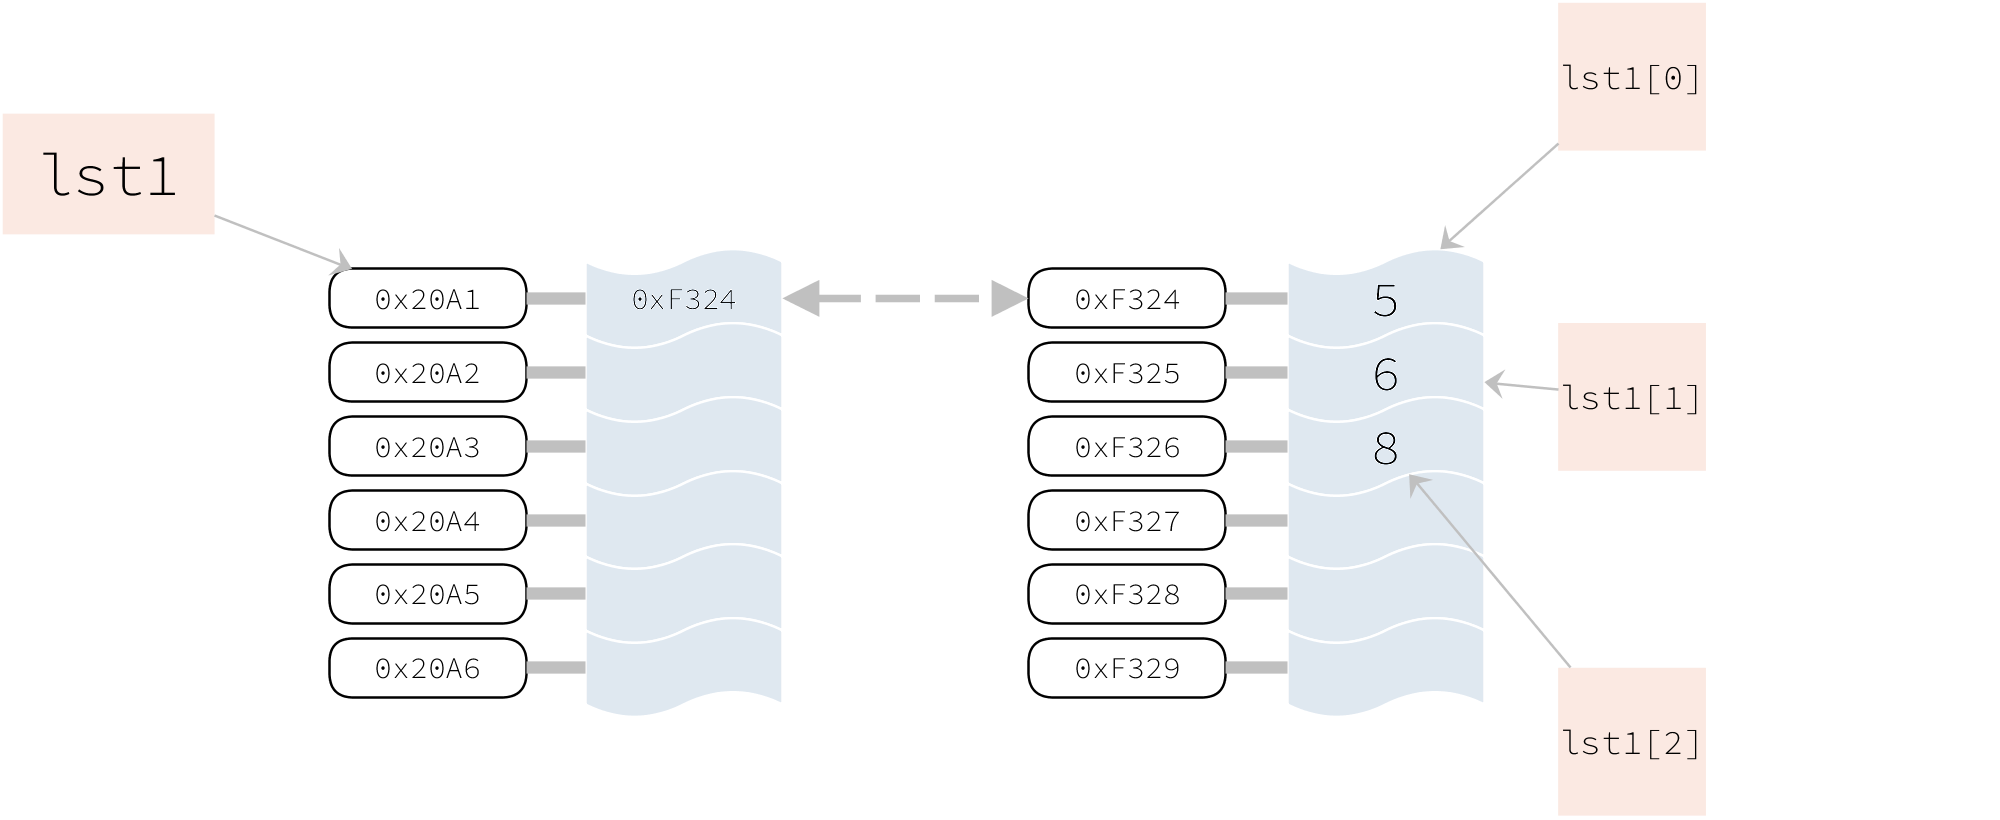
\includegraphics[width=\linewidth]{ch-listes/img/mut1.png}\\


\mintinline{python}{lst2 = lst1}\\

La variable \mintinline{python}{lst2} est associée à la même valeur que \mintinline{python}{lst1}.\\
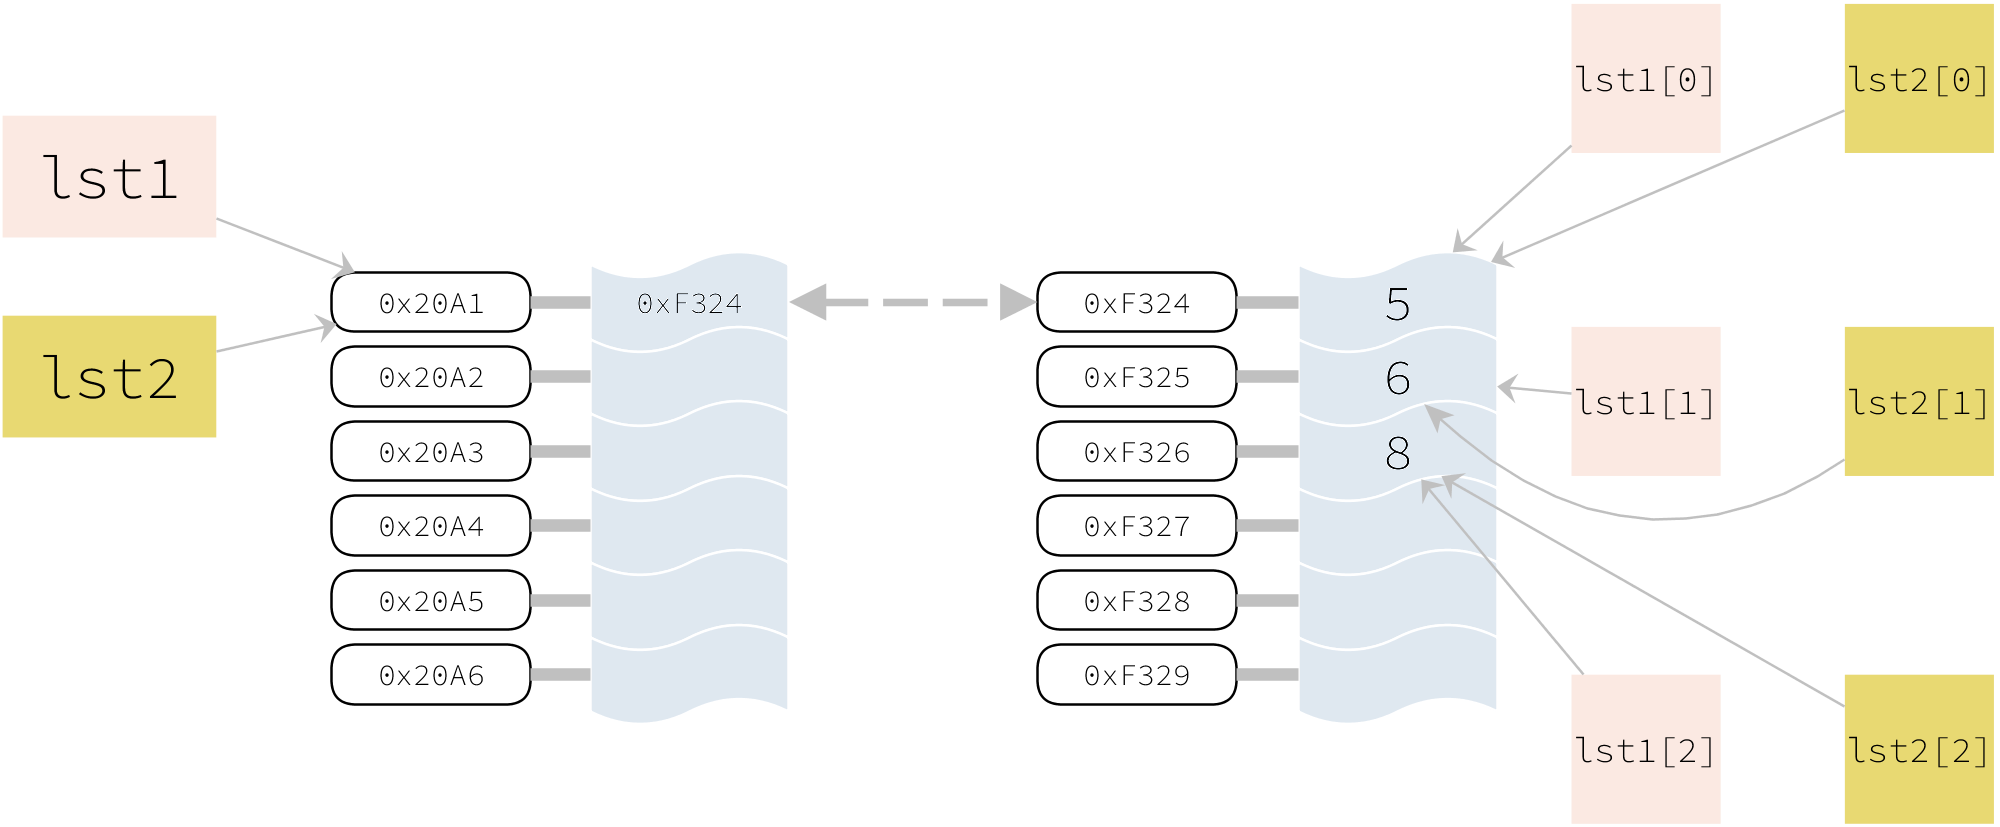
\includegraphics[width=\linewidth]{ch-listes/img/mut2.png}\\


\mintinline{python}{lst1[0] = 10}\\

La valeur de \mintinline{python}{lst1[0]} est changée, elle l'est donc aussi pour \mintinline{python}{lst2}.\\
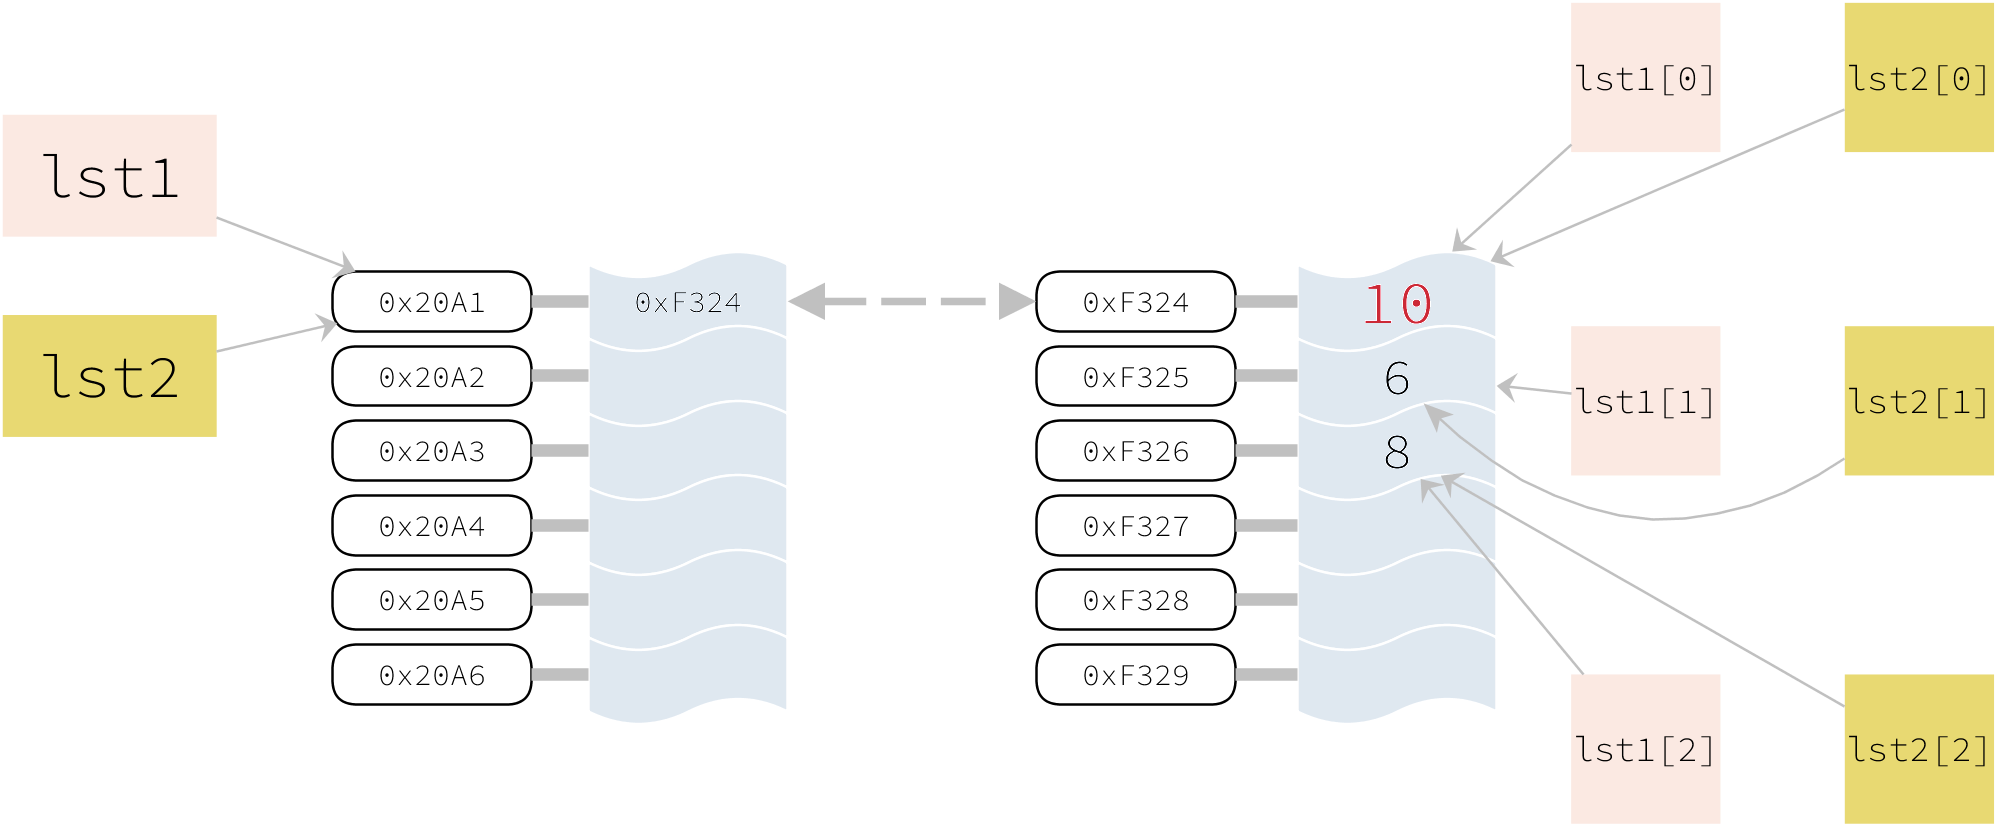
\includegraphics[width=\linewidth]{ch-listes/img/mut3.png} \\
Voilà donc pourquoi lorsqu'on écrit \mintinline{python}{lst2 = lst1}, tout changement dans \mintinline{python}{lst1} se reflète aussi dans \mintinline{python}{lst2} et vice-versa.\\

\subsubsection{Copier une liste (bonne méthode)}



\mintinline{python}{lst2 = lst1[:]}\\

Les éléments de \mintinline{python}{lst1} sont recopiés dans une autre zone mémoire, et \mintinline{python}{lst2} « pointe » sur l'adresse du début de cette zone.\\
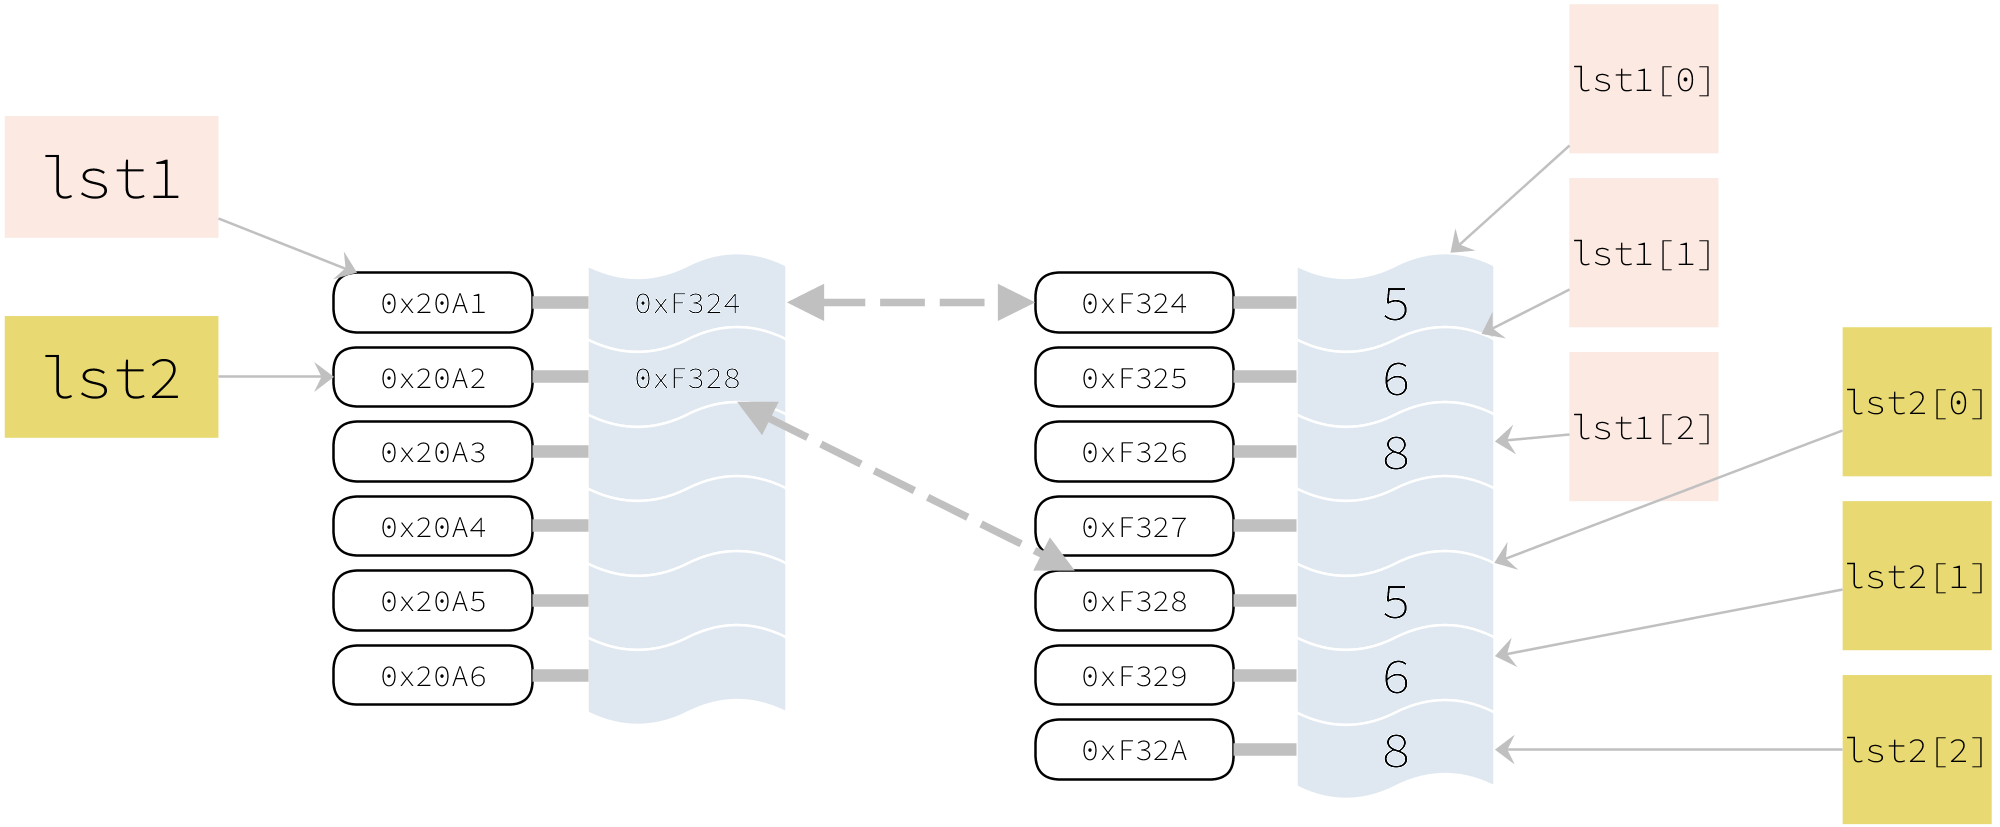
\includegraphics[width=\linewidth]{ch-listes/img/mut4.png}\\


\mintinline{python}{lst1[0] = 10}\\

Le changement n'affecte pas \mintinline{python}{lst2}.\\
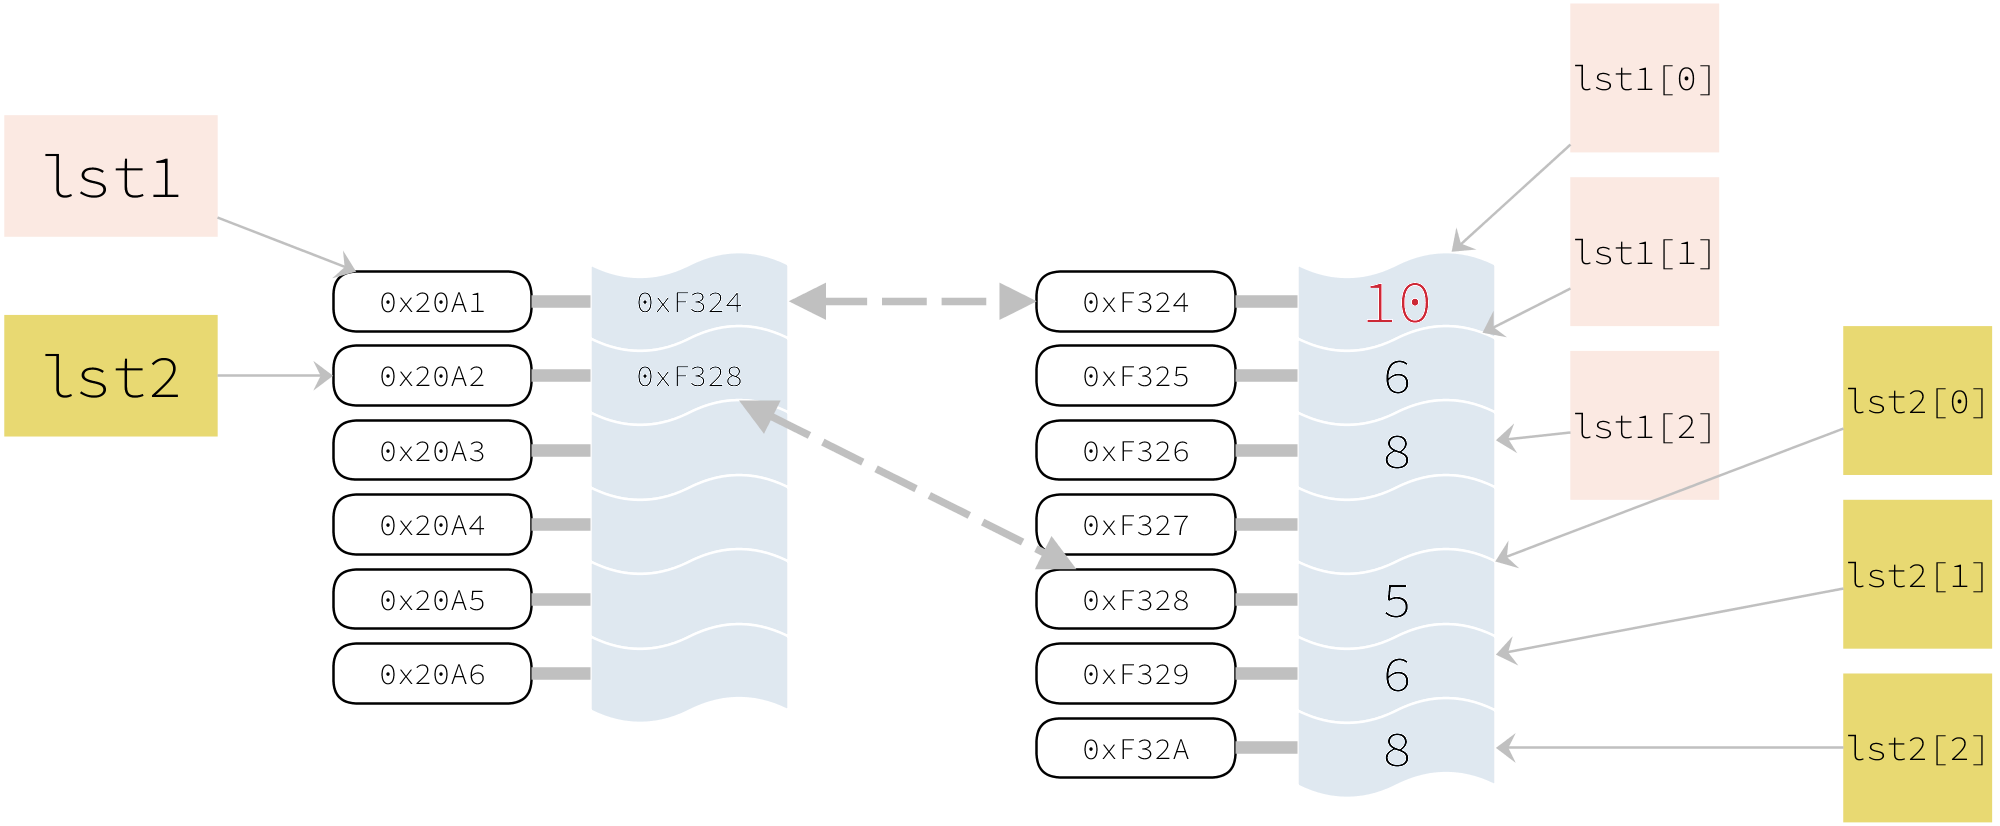
\includegraphics[width=\linewidth]{ch-listes/img/mut5.png}
%  \chapter{Fonctions}
\introduction{Quelle est la fonction de ce chapitre ?}
\section{Exemples de fonctions}
\subsection{Un objet déjà connu}
Nous avons déjà rencontré des fonctions \textit{côté utilisateur}:
\begin{itemize}
    \item \mintinline{python}{input}
          \begin{itemize}
              \item prend en entrée une chaîne de caractères ;
              \item renvoie la chaîne de caractère saisie par l'utilisateur.
          \end{itemize}
          On peut noter ceci \mintinline{python}{input(chaine: str) -> str}
    \item \mintinline{python}{len}
          \begin{itemize}
              \item prend en entrée une liste ;
              \item renvoie le nombre d'éléments de cette liste.
          \end{itemize}
          On peut noter cela \mintinline{python}{len(lst: list) -> int}
\end{itemize}

\subsection{De multiples formes}
\floatpictureright{0.5}{img/fonction1}
{Les deux exemples précédents rentrent dans la catégorie représentée à droite.}
\medskip\par
\floatpictureleft{0.5}{img/fonction2}
{Certaines fonctions sont comme à gauche.\\
    Par exemple \mintinline{python}{max(20,3,10)} renvoie 20.}
\medskip\par
\floatpictureright{0.5}{img/fonction3}{
    D'autres fonctions sont comme à droite.\\
    On verra des exemples plus tard.}
\medskip\par
\floatpictureleft{0.5}{img/fonction4}{
    D'autres encore sont comme à gauche.\\
    Par exemple \mintinline{python}{print("salut")} ne renvoie rien mais affiche \mintinline{python}{salut} à l'écran.}
\medskip\par
\floatpictureright{0.5}{img/fonction5}{
    D'autres suivent le schéma ci-contre.\\
    Par exemple dans le module \mintinline{python}{time}, la fonction \mintinline{python}{time} ne prend aucun paramètre d'entrée mais renvoie l'heure qu'indique l'horloge de l'ordinateur.\\
    On peut par exemple l'utiliser pour stocker une heure précise en tapant \mintinline{python}{maintenant = time()}.}
\medskip\par
\floatpictureleft{0.5}{img/fonction6}{
    Enfin certaines suivent ce schéma.\\
    Par exemple dans le module \mintinline{python}{pygame}, \mintinline{python}{pygame.display.flip} ne prend aucun paramètre d'entrée, ne renvoie aucune valeur, mais actualise la fenêtre graphique.\\
    On l'appelle donc en tapant \mintinline{python}{pygame.display.flip()}.}
\medskip\par
Il est possible de créer de nouvelles fonctions.\\
On parle alors de fonctions \textit{côté concepteur}.\\

Il faut donc définir rigoureusement ce qu'est une fonction.

\section{Définition de la notion de fonction}
\begin{definition}[ : fonction]
    Une \textit{fonction} est un \og morceau de code\fg{} qui représente un \textit{sous-programme}.\\
    Elle a pour but d'effectuer une tâche \textit{de manière indépendante}.\\
\end{definition}

\begin{exemple}
    On veut modéliser la fonction mathématique $f$ définie pour tout nombre réel $x$ par $$f(x)=x^2+3x +2$$

    On écrira alors

    \begin{minted}[breaklines,breakanywhere]{python}
def f(x : float) -> float:
    return x ** 2 + 3 * x + 2
            \end{minted}

    Pour évaluer ce que vaut $f(10)$ et affecter cette valeur à une variable, on pourra désormais écrire \mintinline{python}{resultat = f(10)}.
\end{exemple}


Que fait la fonction \mintinline{python}{mystere} ?

\begin{minted}[breaklines,breakanywhere]{python}
def mystere(a : float, b : float) -> float:
    if a <= b:
        return b
    else:
        return a            
\end{minted}



La fonction \mintinline{python}{mystere}:
\begin{itemize}
    \item   prend en entrée deux paramètres de type \mintinline{python}{float} \mintinline{python}{a} et \mintinline{python}{b};
    \item   renvoie le plus grand de ces deux nombres.
\end{itemize}

La réponse que l'on vient de formuler s'appelle \textit{la spécification} de la fonction $f$.

\begin{definition}[ : fonction]
    Donner la spécification d'une fonction \mintinline{python}{f} c'est
    \begin{itemize}
        \item   préciser le(s) type(s) du (des) paramètre(s) d'entrée (s'il y en a) ;
        \item   indiquer sommairement ce que fait la fonction \mintinline{python}{f} ;
        \item   préciser le(s) type(s) de la (des) valeur(s) de sortie (s'il y en a).
    \end{itemize}
\end{definition}

\section{Anatomie d'une fonction}
\begin{pyc}
\begin{minted}{python}
def f(lst: list) -> int
    mini = lst[0]
    n = len(lst)
    for i in range(n):
        lst[i] < mini:
        mini = lst[i]
    return mini
   \end{minted}
\end{pyc}

La fonction \mintinline{python}{f}
\begin{itemize}
    \item   prend en entrée une liste (sous entendu d'entiers);
    \item   renvoie le plus petit entier de cette liste.
\end{itemize}

\subsection{Paramètre formel}

\floatpictureleft{0.5}{img/anat1}{
Le paramètre d'entrée est \textit{formel} : \textit{le nom de cette variable n'existe qu'à l'intérieur de la fonction}.
Si ce nom de variable existe déjà à l'extérieur de la fonction, \textit{ce n'est pas la même variable}.    
}\medskip\par

\floatpictureright{0.5}{img/anat4}{
Le type du paramètre d'entrée peut être spécifié. Ce n'est pas obligatoire mais très fortement recommandé pour \og garder les idées claires\fg{}.
}\medskip\par

\subsection{Variables locales}
\floatpictureleft{0.5}{img/anat2}{
Toutes les variables \textit{créées} dans une fonction n'existent \textit{que dans cette fonction}. Elles ne sont pas accessibles depuis l'extérieur de la fonction. On dit que ce sont des \textit{variables locales}.}\medskip\par

\subsection{valeur de sortie}
\floatpictureright{0.5}{img/anat3}{
Le type de la valeur de sortie peut être précisé, c'est également recommandé.    
}

\section{En pratique}
\subsection{Des exemples}
 \begin{pyc}
\begin{minted}{python}
1   def f(x : float) -> float:
2       return x ** 2 + 3 * x + 2
3    
4   print(f(1)) # Affiche 6
\end{minted}
\end{pyc}
Le programme commence à la ligne 4 !\\
Les 2 premières lignes servent à définir la fonction \texttt{f}, elles ne sont exécutées que lorsqu'on évalue \texttt{f(1)}.\\



\begin{pyc}
\begin{minted}{python}
def f(x : float) -> float:
    return x ** 2 + 3 * x + 2
    
print(x) # Provoque une erreur
\end{minted}
\end{pyc}
L'erreur vient du fait que la variable \texttt{x} \textit{n'est pas définie}. Le \og \texttt{x} qu'on voit dans la fonction \texttt{f}\fg{} est un paramètre formel et n'existe que dans \texttt{f}.\\


\begin{pyc}
\begin{minted}{python}
def f(x : float) -> float:
    a = 2
    return x + a

print(a) # Provoque une erreur
    \end{minted}
\end{pyc}
L'erreur vient du fait que la variable \texttt{a} \textit{est locale} : elle n'est définie que durant l'exécution de \texttt{f}.\\

\begin{pyc}
\begin{minted}{python}
def f(x : float) -> float:
    a = 2
    return x + a

print(f(4)) # Affiche 6        
print(a) # Provoque une erreur
    \end{minted}
\end{pyc}
C'est encore la même erreur : une fois \texttt{f(4)} évaluée, \texttt{a} n'existe plus.\\

\begin{pyc}
\begin{minted}{python}
1   def f(x : float) -> float:
2       a = 2
3       return x + a
4
5   a = 3
6   print(f(4)) # Affiche 6
7   print(a) # Affiche 3 et pas 2
\end{minted}
\end{pyc}

La variable \texttt{a} définie dans la fonction \texttt{f} n'est pas la même que celle qui est définie à la ligne 5.\\
Celle définie à la ligne 2 est \textit{locale}.\\
La variable \texttt{a} de la ligne 5 est appelée \textit{globale}.\\



\begin{pyc}
\begin{minted}{python}
def f(x : float) -> float:
    return x + a
        
a = 3
print(f(4)) # Affiche 7
\end{minted}
\end{pyc}
\begin{aretenir}
Une fonction a le droit d'\textit{accéder en lecture} à une variable globale, mais n'a pas \textit{a priori} le droit d'en modifier la valeur.
\end{aretenir}

\subsection{À éviter autant que possible}



\begin{pyc}
\begin{minted}{python}
1   def f(x : float) -> float:
2       global a 
3       a = a + 1
4       return x + a
5        
6   a = 3
7   print(f(4)) # Affiche 8
8   print(a) # Affiche 4       
\end{minted}
\end{pyc}
À la ligne 2, on signale à Python que \texttt{f} a la droit de modifier la variable globale \texttt{a}.
C'est fortement déconseillé : sauf si on ne peut pas faire autrement, une fonction ne doit pas modifier les variables globales.
%  \chapter{\'Ecriture en compréhension}

\section{\'Ecritures simples}

Jusqu'à présent, pour construire des listes on a souvent :
\begin{itemize}
    \item    créé une liste \mintinline{python}{lst} vide ;
    \item    construit une boucle \mintinline{python}{for} ou \mintinline{python}{while} ;
    \item    peuplé la liste avec \mintinline{python}{lst.append}.
\end{itemize}

\begin{exemple}[]
    \begin{minted}{python}
        lst = []
        for i in range(10):
            lst.append(i*i)
        print(lst)
    \end{minted}
\end{exemple}


Ce programme affiche \mintinline{python}{[0, 1, 4, 9, 16, 25, 36, 49, 64, 81]}\\
C'est la liste des carrés des 10 premiers entiers naturels.\\
En mathématiques, l'ensemble des carrés des 10 premiers entiers naturels se note
\[\left\lbrace i^2\ |\ i\in\N,\,i<10\right\rbrace\]
C'est une écriture en \textit{compréhension}.\\
On peut faire la même chose en \textsc{Python} : \\

\mintinline{python}{lst = [i*i for i in range(10)]}\\

\'Evidemment, c'est plus rapide que la méthode précédente... Et on peut faire bien plus !
On peut utiliser une liste pour en construire une autre, par exemple en ajoutant 1 à chacun des éléments :
\begin{pyc}
    \begin{minted}{python}
    >>> lst1 = [2, -1, 3, 4, 7]
    >>> lst2 = [x + 1 for x in lst1]
    >>> lst2
    [3, 0, 4, 5, 8]
    \end{minted}
\end{pyc}
Dans le même esprit, on peut construire une liste dont les élements sont ceux de la première, mais avec une conversion de type :

\begin{pyc}
\begin{minted}{python}
>>> lst1 = ['2', '0', '13']
>>> lst2 = [int(x) for x in lst1]
>>> lst2
[2, 0, 13]
\end{minted}
\end{pyc}


Ou encore fabriquer la liste des initiales à partir d'une liste de prénoms :
\begin{pyc}
\begin{minted}{python}
>>> lst1 = ['Fred', 'Titouan', 'Tinaïg']
>>> lst2 = [prenom[0] for prenom in lst1]
>>> lst2
['F', 'T', 'T']
\end{minted}
\end{pyc}

\section{\'Ecritures avec conditions}



Il est possible d'utiliser \mintinline{python}{if} en compréhension : mettons dans \mintinline{python}{lst2} le double de chaque élément de \mintinline{python}{lst1} supérieur à 10 (dans l'ordre de parcours).
\begin{pyc}
\begin{minted}{python}
l>>> lst1 = [8, 0, 11, 10, 3, 15]
>>> lst2 = [2 * x for x in lst1 if x > 10]
>>> lst2
[22, 30]
\end{minted}
\end{pyc}



Il est possible d'utiliser \mintinline{python}{if ... else ...} en compréhension, mais à ce moment là il faut écrire les conditions au début   : créons une nouvelle liste en remplaçant tous les nombres négatifs de \mintinline{python}{lst1} par zéro.
\begin{pyc}
\begin{minted}{python}
>>> lst1 = [8, -10, 11, -4, -3, 15]
>>> lst2 = [(x if x > 0 else 0) for x in lst1]
# les parenthèses sont facultatives
>>> lst2
[8, 0, 11, 0, 0, 15]
\end{minted}
\end{pyc}

Créons une liste contenant les indices des éléments de \mintinline{python}{lst1} qui sont strictement positifs.
\begin{pyc}
\begin{minted}{python}
>>> lst1 = [8, -10, 11, -4, -3, 15]
>>> lst2 = [i for i in range(len(lst1)) if lst1[i] > 0]
>>> lst2
[0, 2, 5]
\end{minted}
\end{pyc}

\section{Les écritures en compréhension imbriquées}

$$\begin{matrix}
        0 & 0 & 0 & 0 \\0 & 0 & 0 & 0 \\0 & 0 & 0 & 0
    \end{matrix}$$
Si on veut représenter ce « tableau de nombres » par une liste, on peut écrire cet liste de 3 lignes comportant chacune 4 éléments :\\

\mintinline{python}{lst = [[0, 0, 0, 0], [0, 0, 0, 0], [0, 0, 0, 0]]}.\\

Cependant il est plus pratique d'écrire\\

\mintinline{python}{lst=[[0 for j in range(4)] for i in range(3)]}

\section{Pour conclure}

On peut combiner toutes les techniques que nous venons de voir. Par exemple on peut créer une liste de listes de listes avec des conditions, \textit{et c\ae tera}. La seule limite, c'est l'imagination et la capacité à écrire en \textsc{Python} !

%  \chapter{Dictionnaires}
\section{Un nouveau type}

\floatpictureright{0.3}{ch-dictionnaires/img/dico}{
    On demande à des jeunes quel est leur sport préféré, les résultats sont présentés sur la figure ci-contre.\\
    Un sport peut être cité par \textit{plusieurs} jeunes, en revanche chaque jeune ne peut citer qu'\textit{un seul} sport.\\
    On pourrait utiliser une ou plusieurs listes pour représenter ces données mais il y a mieux : le \textit{dictionnaire}.
    La variable \mintinline{python}{sport} est de type \mintinline{python}{dict} :
}
\begin{pyc}
    \begin{minted}{python}
        sport = {'A': 'Tennis', 'B': 'Basket',
                 'C': 'Judo', ' D': 'Boxe',
                 'E': 'Foot', 'F': 'Gym',
                 'G': 'Foot'}
        \end{minted}
\end{pyc}


\begin{definition}[ : dictionnaire]
    Un dictionnaire est un ensemble d'\textit{éléments}.\\
    les éléments sont des couples de la forme \textit{clé : valeur}.\\

    La syntaxe est :\\ \mintinline{python}{variable = { cle1 : valeur1, cle2 : valeur2, ...}}\\

    Les valeurs peuvent être de n'importe quel type. Les clés peuvent être
    \begin{itemize}
        \item 	des \mintinline{python}{bool}, des \mintinline{python}{int}, des \mintinline{python}{float};
        \item 	des \mintinline{python}{str}...
        \item 	mais pas des \mintinline{python}{list} !
    \end{itemize}
\end{definition}


On peut tout de même utiliser des \mintinline{python}{tuples} en guise de clés :  les \mintinline{python}{tuples} ressemblent aux \mintinline{python}{list} mais sont \textit{non mutables}.\\

\mintinline{python}{a = (1, 2, 3)} est un exemple de \mintinline{python}{tuple}.

\section{Opérations sur les dictionnaires}

\subsection{Accéder à une valeur par sa clé}
Pour connaître le sport préféré de \mintinline{python}{'A'}, c'est simple :
\begin{pyc}
    \begin{minted}{python}
>>> sport['A']
'Tennis'        
    \end{minted}
\end{pyc}


\subsection{Créer de nouveaux couples clé: valeur}

Contrairement aux listes, il n'y a pas de méthode \texttt{append}.\\
Pour intégrer l'information « le sport préféré de H est le Rugby » on écrira simplement :\\
\begin{pyc}
    \begin{minted}{python}
        >>> sport['H']='Rugby'
    \end{minted}
\end{pyc}


\subsection{Créer un dictionnaire vide et le peupler}

On peut partir d'un dictionnaire vide et remplir ses valeurs au fur et à mesure :

\begin{pyc}
    \begin{minted}{python}
        >>> d = dict()
        >>> d['bonjour'] = 'hello'
        >>> d['crayon'] = 'pencil'
        >>> d['se prélasser'] = 'to bask'
    \end{minted}
\end{pyc}
\subsection{Supprimer un élément du dictionnaire}

\mintinline{python}{del d['crayon']} supprime l'élément \mintinline{python}{'crayon': 'pencil'}.

\subsection*{fusionner 2 dictionnaires}
\begin{minted}{python}
>>> d1 = {"anglais": "bread", 
          "français": "pain", 
          "slovaque": "chlieb"}
>>> d2 = {"allemand": "brot", "italien": "pane"}
>>> d1.update(d2) # fusionne d2 dans d1
>>> d1
{"anglais": "bread", "français": "pain", "slovaque": "chlieb", "allemand": "brot", "italien": "pane"}
\end{minted}

\subsection{Parcourir l'ensemble des clés d'un dictionnaire}
\begin{pyc}
    \begin{minted}{python}
    for cle in d1.keys():
        print(cle)
    \end{minted}
\end{pyc}
Ce script affiche
\begin{minted}{python}
anglais
français
slovaque
allemand
italien
\end{minted}

\subsection{Parcourir l'ensemble des valeurs d'un dictionnaire}
\begin{pyc}
    \begin{minted}{python}
for valeur in d1.values():
    print(valeur)
\end{minted}
\end{pyc}
Ce script affiche
\begin{minted}{python}
bread
pain
chlieb
brot
pane
\end{minted}

\subsection{Précisions}
\mintinline{python}{d1.keys()} et \mintinline{python}{d1.values()} ressemblent à des listes mais n'en sont pas !\footnote{Ce sont des \textit{itérateurs}, sctructures destinées à être parcourues. }\\

Pour avoir par exemple la liste des clés de \mintinline{python}{d1} on écrira :\\

\mintinline{python}{list(d1.keys())}\\

ou bien en \textit{compréhension} (ce qui revient au même mais peut s'avérer utile)

\mintinline{python}{[k for k in d1.keys()]}

\subsection{Erreurs de clé}
\begin{minted}{python}
print(d1['suédois'])
\end{minted}

Ce script produit une erreur :

{\color{red}\texttt{KeyError : 'suédois'}}

\begin{exemple}[ : Utilisation d'un dictionnaire]
    On veut créer un tableau de $10\times 10$ cases avec la valeur 0 dedans.\\

    On peut bien sûr créer cela avec une liste de listes (en compréhension) mais on peut également utiliser un dictionnaire :\\

    \mintinline{python}{{(x, y) : 0 for x in range(1, 11) for y in range(1, 11)}}\\

    \textbf{Avantages :}
    \begin{itemize}
        \item 	plus simple à manipuler : on écrit \mintinline{python}{d[x, y]} au lieu de \mintinline{python}{d[x][y]} ;
        \item 	on n'est pas obligé de faire commencer les indices à zéro.
    \end{itemize}

    \textbf{Inconvénients :}
    \begin{itemize}
        \item prend plus de place en mémoire (on s'en fiche un peu) ;
        \item plus flexible entraîne plus de possibilité d'erreurs !
    \end{itemize}
\end{exemple}


\section{Utilisation des dictionnaires}


Typiquement, pour stocker des \textit{données structurées} :    \\
\begin{minted}{python}
reseau = {'nom'        : 'local',
          'ip'         : '192.168.1.0',
          'masque'     : '255.255.255.0',
          'passerelle' : '192.168.1.254'}
\end{minted}

On utilise fréquemment des listes de dictionnaires, ou bien des dictionnaires de listes.


% % \part{Algorithmique}

\chapter{Complexité}
\section{Des exemples}

Voici trois exemples de problèmes qu'on peut vouloir résoudre 

\subsection{Test de primalité}
    Étant donné un entier $n$ plus grand que 1, cet entier est-il premier\footnote{\noindent est-ce qu'il existe d'autres diviseurs de $n$ que $1$ et $n$ ?} ou non ?\medskip

    Par exemple, 127 est-il premier ? Pour y répondre, on va diviser 127 par 2, par 3, par 4, \textit{et cætera}, et regarder si une de ces divisions « tombe juste » ou non. Si c'est le cas, 127 n'est pas premier. On n'a pas besoin de pousser les divisions jusqu'à 126, il suffit simplement d'aller jusqu'à $\lfloor\sqrt{127}\rfloor$, c'est-à-dire onze\footnote{\noindent en effet, si $n$ admet un diviseur, alors on peut écrire $n=pq$ avec $p$ et $q$ deux entiers et il y en a obligatoirement un des deux qui est plus petit ou égal à $\sqrt{n}$, donc à $\lfloor\sqrt{n}\rfloor$ puisqu'il est entier.}.\\
    Quand on le fait, on se rend compte que 127 est premier.

\subsection{Recherche de la présence d'un élément dans une liste}
    Étant donnée une liste d'entiers \mintinline{python}{lst} de longueur $n$ et un entier \mintinline{python}{val}, cet entier appartient-il ou non à \mintinline{python}{lst} ?\medskip

    Par exemple, avec une liste \mintinline{python}{lst} valant \mintinline{python}{[4, 2, 7, 8, 9]} et une valeur \mintinline{python}{val} de \mintinline{python}{5}, il faut parcourir \textit{intégralement} \mintinline{python}{lst} pour constater que \mintinline{python}{val} n'y figure pas.

\subsection{Table de multiplication}
    Étant donné un entier $n\in\N^*$, on veut afficher tous les nombres de la forme $i\times j$, avec $i$ et $j$ entiers compris entre 1 et $n$.\medskip

    Par exemple pour $n$ valant 4, j'obtiens la table suivante :
    \begin{center}
    \tabularstyled
    \begin{tabular}{c|c|c|c}
    1 & 2 & 3 & 4\\
    2 & 4 & 6 & 8 \\
    3 & 6 & 9 & 12 \\
    4 & 8 & 12 & 16            
    \end{tabular}
    \end{center}


Pour chacune des situations précédentes, $n$ est appelé \textit{taille du problème}. Plus $n$ augmente, plus le nombre d'opérations (au sens large : calculs, tests, accès aux éléments d'une liste, \textit{et cætera}) augmente.\\

À quelle vitesse ce nombre d'opérations augmente-t-il ?\\

S'il y a plusieurs algorithmes pour résoudre un même problème, y en a-t-il un plus efficace que les autres, c'est-à-dire dont le nombre d'opérations augmente moins vite lorsque $n$ augmente ?

\section{Complexité temporelle}

Évaluer la complexité temporelle d'un algorithme, c'est estimer le nombre d'opérations \textit{significatives} qui entrent en jeu lors de la résolution par cet algorithme d'un problème de taille $n$. 

\begin{methode}[ : évaluation de la complexité temporelle]
Pour évaluer l'efficacité d'un algorithme en terme de nombre d'opérations
\begin{itemize}
   \item    d'abord on décide ce qu'est une opération significative. On appelle ceci une \textsc{opel} ; 
   \item    seules les \textsc{opel} sont considérées comme coûteuses en temps et sont comptabilisées ;
   \item    les autres opérations sont \textit{négligées} ;
   \item    on cherche à estimer le nombre d'\textsc{opel} nécessaires à la résolution par l'algorithme d'un problème de taille $n$. 
\end{itemize}
\end{methode}                                   


On peut « imaginer » une fonction $c_M$ (au sens mathématique du terme) qui serait définie pour toute taille $n$ du problème et	donnerait le nombre \textit{moyen}  d'\textsc{opel} nécessaires pour résoudre un problème de taille $n$.\\
Cette \textit{complexité moyenne} est très rarement calculable car les calculs trop compliqués.\\


Plus simple mais tout aussi utile que $c_M$, est la complexité \textit{dans le pire des cas}.

\begin{definition}[ : complexité dans le pire des cas]
Pour un problème de taille $n$, on note $c(n)$ le nombre maximal d'\textsc{opel} pour résoudre un problème de cette taille.
\end{definition}

En pratique, on ne calcule pas \textit{exactement} $c(n)$. On se contente d'indiquer à quelle vitesse $c(n)$ augmente lorsque $n$ augmente, en se servant de \textit{fonctions de référence} telles que celles représentées ci-dessous.\\

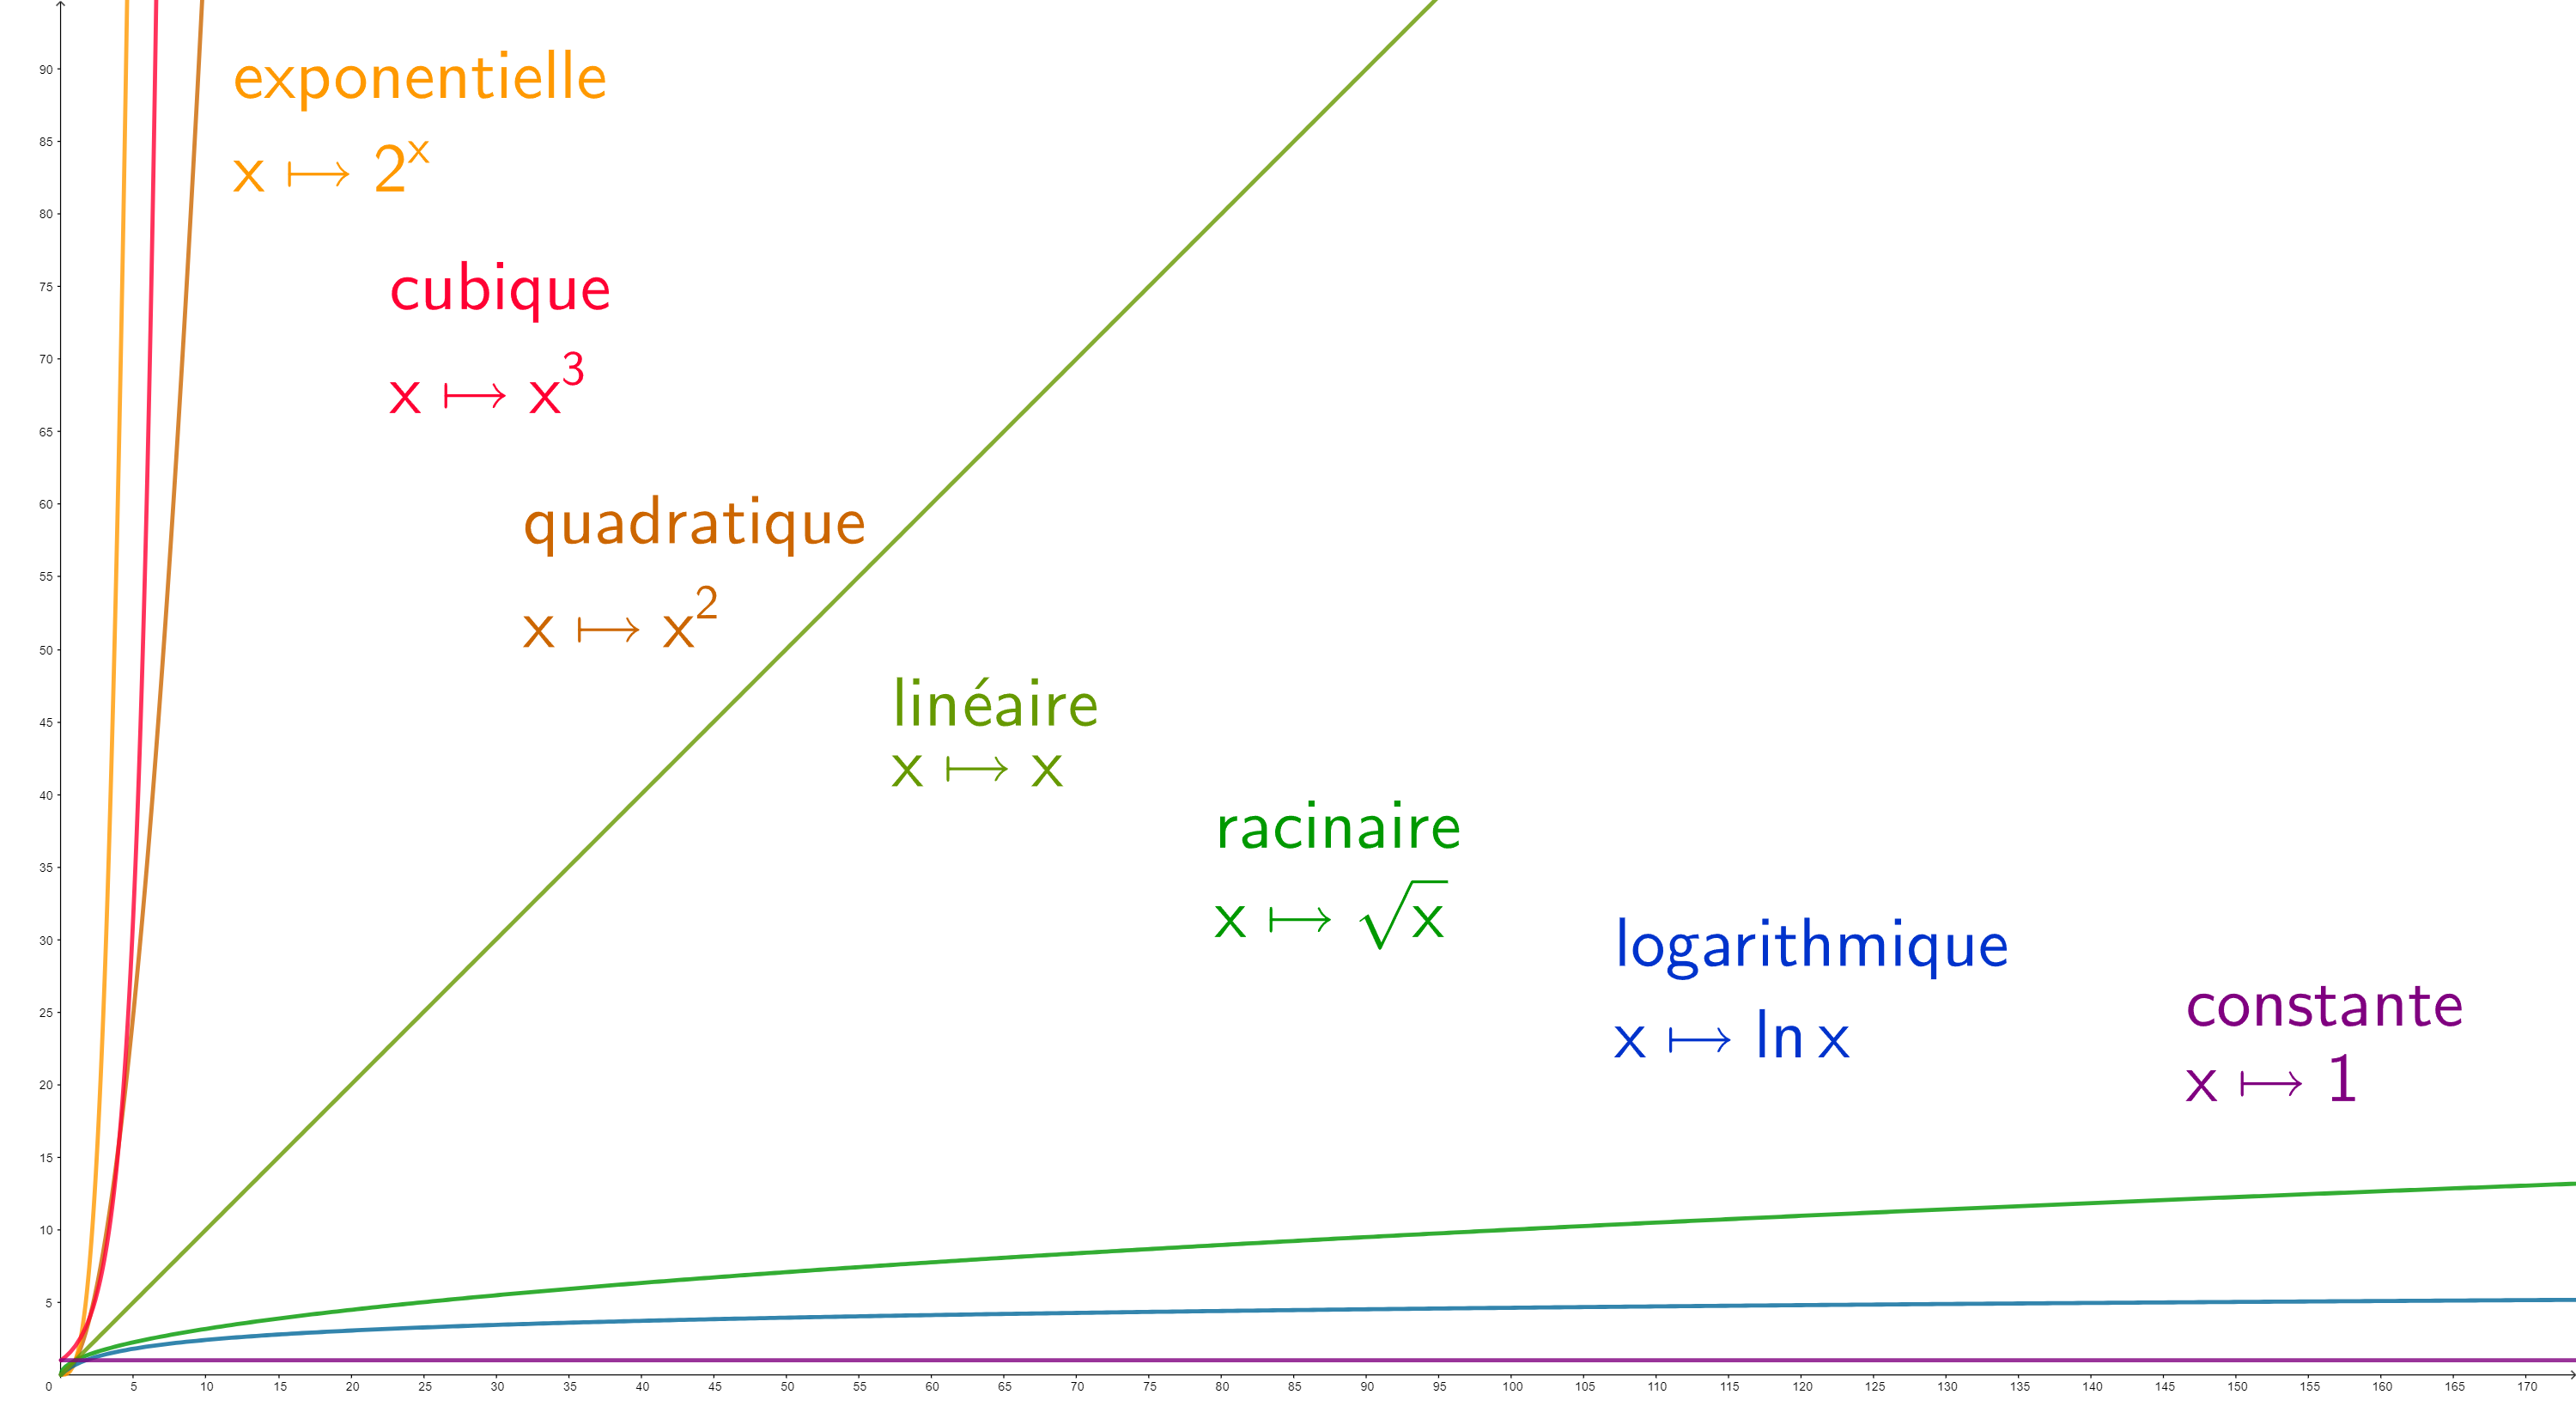
\includegraphics[width=\linewidth]{ch-complexite/img/complexite}

Il est très utile de connaître la complexité d'un algorithme car cela nous permet d'estimer le temps de resolution d'un problème quand on connaît l'ordre de grandeur de $n$ comme le montre le tableau ci-dessous.
\begin{center}

\tabularstyled
\renewcommand{\arraystretch}{1.5}
\scriptsize
\begin{tabular}{c|c|c|c|c|c|c|c|c}
\rowcolor{UGLiOrange}
& {\boxfont\color{white}5} & {\boxfont\color{white}10} & {\boxfont\color{white}20} & {\boxfont\color{white}50} & {\boxfont\color{white}250} & {\boxfont\color{white}1 000} & {\boxfont\color{white}10 000} & {\boxfont\color{white}1 000 000} \\
constante & 10 ns & 10 ns & 10 ns & 10 ns & 10 ns & 10 ns & 10 ns & 10 ns \\
logarithmique & 10 ns & 10 ns & 10 ns & 20 ns  & 30 ns & 30 ns & 40 ns & 60 ns \\
racinaire & 22 ns & 32 ns & 45 ns & 71 ns & 158 ns & 316 ns & 1 µs & 10 µs \\
linéaire & 50 ns & 100 ns & 200 ns & 500 ns & 2,5 µs & 10 µs & 100 µs & 10 ms \\
quadratique & 250 ns & 1 µs & 4 µs & 25 µs & 625 µs & 10 ms & 1 s & 2,8 h \\
cubique & 1,25 µs & 10 µs & 80 µs & 1.25 ms & 156 ms & 10 s & 2,7 h & 316 ans \\
exponentielle & 320 ns & 10 µs & 10 ms & 130 jours & $10^{59}$ ans & \ldots & \ldots & \ldots \\
\end{tabular}
\renewcommand{\arraystretch}{1}
\end{center}


\section{Application à nos exemples}

\subsection{Test de primalité}

\begin{pyc}
   \begin{minted}{python}
      from math import sqrt
      def est_premier(n: int) -> bool:
         # on parcourt les entiers de 2 à racine(n)
         for i in range(2, int(sqrt(n)) + 1):
            # si une division tombe juste
            if n % i == 0:
               # alors n n'est pas premier
               return False
         # si aucune ne tombe juste il est premier
         return True
   \end{minted}
\end{pyc}

On convient qu'une \textsc{opel} est une division. Pour $n$ fixé, on effectue au pire des cas les divisions par 2, 3, \ldots, $\lfloor\sqrt{n}\rfloor$, il y en a \textit{grosso modo} $\sqrt{n}$ : notre algorithme est de complexité racinaire\footnote{en réalité c'est sans doute plus que cela car plus $n$ est grand, plus les nombres qui entrent en jeu dans les divisions sont grands et plus les divisions prennent de temps.}. 

\subsection{Recherche de la présence d'un élément dans une liste}

\begin{pyc}
   \begin{minted}{python}
      def present(lst: list, val: int) -> bool:
         # on parcourt la liste par ses éléments
         for x in lst:
            # si on trouve val
            if x == val:
               # on renvoie True
               return True
         # si on ne l'a pas trouvé, on renvoie False
         return False
   \end{minted}
\end{pyc}
Ici une \textsc{opel} sera un accès à un élément de la liste, c'est à dire le fait d'attribuer les valeurs à la variable \mintinline{python}{x}. Pour une liste de taille $n$ fixé, dans le pire des cas \mintinline{python}{val} n'appartient pas à \mintinline{python}{lst} et on effectue $n$ \textsc{opel} : notre algorithme est de complexité linéaire.

\subsection{Table de multiplication} 

\begin{pyc}
   \begin{minted}{python}
      def affiche(n: int) -> None:
         for i in range(1, n + 1):
            for j in range(1, n + 1):
               print(i * j)
   \end{minted}
\end{pyc}

Ici une \textsc{opel} est une multiplication. Pour $n$ fixé, dans tous les cas on effectue deux boucles imbriquées, donc $n\times n$ sont effectuées et notre algorithme est de complexité quadratique.

\section{Exercices}
\begin{exercice}
   Une \textsc{opel} est une addition, déterminer la complexité de la fonction suivante:
   \begin{minted}{python}
   def somme(n: int) -> int:
      s = 0
      for i in range(1, n + 1):
         s += i
      return s
    \end{minted} 
\end{exercice}

\begin{exercice}[ : nombre de bits d'un entier]
   La fonction suivante 
   \begin{itemize}
      \item prend en entrée un \mintinline{python}{n} non nul ;
      \item renvoie le nombre de bits nécessaires à l'écriture de $n$ en base 2. 
   \end{itemize}
   
   \begin{minted}{python}
   def nb_bits(n: int) -> int:
   b = 0
   while n > 0:
      b += 1
      n = n // 2
   return b
   \end{minted}
   Une \textsc{opel} est une division par 2. En testant la fonction \mintinline{python}{nb_bits} sur des entiers de plus en plus grands, conjecturer la complexité de cette fonction. 

\end{exercice}

\begin{exercice}[* : addition de matrices]
   On considère des \textit{matrices}, qui sont représentées par des listes de listes d'\mintinline{python}{int} ($n$ lignes et $n$ colonnes).
   Par exemple les matrices 
   \tabulardefault
   $$M_1 = \begin{matrice}
         1 & 2 & -1\\
         0 & -1 & 2\\
         -1& 1 & 0\\
   \end{matrice}\quad\text{et}\quad M_2 = \begin{matrice}
         -3 & 1 & 0\\
         1 & 0 & -2\\
         1& -1 & 1\\
   \end{matrice}$$
   sont deux matrices carrées d'ordre 3 et sont représentées en \textsc{Python} par \\
   \mintinline{python}{m1 = [[1, 2, -1], [0, -1, 2], [-1, 1, 0]]} et\\
   \mintinline{python}{m2 = [[-3, 1, 0], [1, 0, -2], [1, -1, 1]]}\\

   Il est possible d'ajouter 2 matrices de même taille en procédant « case par case »  :
   $$M_1+M_2 = \begin{matrice}
         -2 & 3 & -1\\
         1 & -1 & 0\\
         0& 0 & 1\\
   \end{matrice}$$
   En convenant qu'une \textsc{opel} est une addition de deux \mintinline{python}{int} , sans écrire l'algorithme, donner la complexité de l'algorithme d'addition de deux matrices.
\end{exercice}
\begin{exercice}[* : multiplication de matrices]
   Il est possible de multiplier 2 matrices de même taille suivant l'algorithme suivant :
  
      \begin{minted}{python}
         def produit(m1: list, m2: list) -> list:
            # n est la taille des matrices
            n = len(m1) 
            # on crée une matrice remplie de zéros
            p = [[0 for j in range(n)] for i in range(n)]
            # pour chaque ligne
            for i in range(n):
               # pour chaque colonne
               for j in range(n):
                  # on ajoute tous ces nombres
                  for k in range(n):
                     p[i][j] += m1[i][k] * m2[k][j]
            # puis on renvoie la matrice produit
            return p
      \end{minted}


   Déterminer la complexité de cet algorithme.
\end{exercice}

%  
\chapter{Recherche dichotomique}
\introduction{Plus petit ou plus grand ?}

\section{Présentation de l'algorithme}

Lorsqu'on cherche si un élément appartient ou non à une liste, il suffit de la parcourir en comparant chacun de ses éléments à celui que l'on cherche.

Cette démarche peut être améliorée si la liste possède des propriétés particulières, notamment si c'est une liste d'entiers triée.


On veut écrire une fonction \texttt{recherche\_dichotomique} qui :

En entrée prend \begin{itemize}
	\item 	une liste \mintinline{python}{liste_triee} de $n$ entiers \textit{triée dans l'ordre croissant};
	\item 	un entier \mintinline{python}{val}.
\end{itemize}
Renvoie \begin{itemize}
	\item 	l'indice de \mintinline{python}{val} dans \mintinline{python}{liste_triee} si \mintinline{python}{val} appartient à \mintinline{python}{liste_triee};
	\item 	-1 si a n'appartient pas à \mintinline{python}{liste_triee}.
\end{itemize}



\begin{exemple}[]
	\begin{itemize}
		\item 	\mintinline{python}{recherche_dichotomique([11, 20, 32, 33, 54], 32)} \\renvoie 2 car 32 est l'élément d'indice 2 de la liste.
		\item 	\mintinline{python}{recherche_dichotomique([20, 32, 33, 54], 40)} \\renvoie -1 car 40 ne figure pas dans la liste.
	\end{itemize}
\end{exemple}

\begin{methode}[]
	On compare \mintinline{python}{val} avec l'élément \mintinline{python}{m} qui se situe « à peu près au milieu de \mintinline{python}{liste_triee} ».
	\begin{itemize}
		\item 	si \mintinline{python}{val} est égal à \mintinline{python}{m} c'est gagné, on renvoie l'indice de \mintinline{python}{m} dans  \mintinline{python}{liste_triee};
		\item 	sinon si \mintinline{python}{val > m} on recommence avec la liste des éléments situés après \mintinline{python}{m}.
		\item 	sinon c'est que \mintinline{python}{val < m} et on recommence avec la liste des éléments situés avant \mintinline{python}{m}.
	\end{itemize}
	On itère ce procédé tant que la liste des valeurs à examiner n'est pas vide. Si on arrive à une liste vide c'est que \mintinline{python}{val} , n'est pas dans \mintinline{python}{liste_triee}.
\end{methode}
Voici l'algorithme traduit en \textsc{Python} :
\begin{pyc}
			\begin{minted}{python}
01	def recherche_dichotomique(liste_triee, val):
02		# début de la plage de valeurs à regarder
03		gauche = 0  
04		# fin de la plage
05		droite = len(liste_triee) - 1
06		# tant que la plage est non vide  
07		while gauche <= droite:  
08			# on prend grosso modo le milieu
09			milieu = (gauche + droite) // 2  
10			# si on trouve val au milieu c'est gagné
11			if liste_triee[milieu] == val:
12				return milieu  
13			# si on a dépassé val
14			elif liste_triee[milieu] > val:  
15				# alors on regarde avant
16				droite = milieu - 1  
17			# sinon on regarde après
18			else:
19				gauche = milieu + 1  
20		# si on est sorti de la boucle
21		# c'est qu'on n'a pas trouvé val
22		return -1  
	\end{minted}
\end{pyc}

\section{Comprendre l'algorithme}

Commençons par le faire « tourner à la main » sur un exemple, avec\\ \mintinline{python}{liste_triee} valant \mintinline{python}{[1, 3, 4, 8, 9, 13, 20, 21]} .\\

On cherche la valeur 4.\\

Pour chaque itération on a noté dans un tableau les valeurs des variables (celles de \mintinline{python}{gauche} et \mintinline{python}{droite} avant qu'elles ne soient modifiées) et si la fonction renvoie quelque chose ou non.

\begin{center}
	\small
	\tabularstyled
	\begin{tabular}{|c|c|c|c|c|c|}
		\hline
		\rowcolor{UGLiOrange}{\ccell   n° d'itér} & {\ccell   gauche} & {\ccell   droite} & {\ccell   milieu} & {\ccell   liste\_triee[milieu]} & {\ccell   valeur renvoyée} \\
		\hline
		1                                                     & 0                             & 7                             & 3                             & 8                                           & NON                                    \\
		\hline
		2                                                     & 0                             & 2                             & 1                             & 3                                           & NON                                    \\
		\hline
		3                                                     & 2                             & 2                             & 2                             & 4                                           & OUI : 2                                \\
		\hline
	\end{tabular}
\end{center}
Ainsi la fonction a renvoyé 2, indice de la valeur 4 dans la liste, au bout de 3 itérations.\\

On cherche la valeur 15:
\begin{center}
	\tabularstyled
	\begin{tabular}{|c|c|c|c|c|c|}
		\hline
		\rowcolor{UGLiOrange}{\ccell  n°itér} & {\ccell  gauche} & {\ccell  droite} & {\ccell  milieu} & {\ccell  liste\_triee[milieu]} & {\ccell  return ?} \\
		\hline
		1                                                  & 0                             & 7                             & 3                             & 8                                           & NON                             \\
		\hline
		2                                                  & 4                             & 7                             & 5                             & 13                                          & NON                             \\
		\hline
		3                                                  & 6                             & 7                             & 2                             & 20                                          & NON                             \\
		\hline
		-                                                  & 7                             & 6                             & -                             & -                                           & OUI : -1                        \\
		\hline
	\end{tabular}
\end{center}
La dernière ligne du tableau signifie qu'au bout de la 3\eme itération, les conditions de boucles ne sont plus vérifiées (car \mintinline{python}{gauche > droite}) et que -1 est renvoyé.
\begin{exercice}

	On cherche la valeur 6 dans la liste précédente.

	Complète le tableau (des lignes resteront peut-être vides).
	\begin{center}
		\tabularstyled
		\begin{tabular}{|c|c|c|c|c|c|}
			\hline
			\rowcolor{UGLiOrange}{\ccell  n°itér} & {\ccell  gauche} & {\ccell  droite} & {\ccell  milieu} & {\ccell  liste\_triee[milieu]} & {\ccell  return ?} \\
			\hline
			                                                   &                               &                               &                               &                                             &                                 \\
			\hline
			                                                   &                               &                               &                               &                                             &                                 \\
			\hline
			                                                   &                               &                               &                               &                                             &                                 \\
			\hline
			                                                   &                               &                               &                               &                                             &                                 \\
			\hline
		\end{tabular}
	\end{center}

	On cherche la valeur 21, complète le tableau (des lignes resteront peut-être vides).
	\begin{center}
		\tabularstyled
		\begin{tabular}{|c|c|c|c|c|c|}
			\hline
			\rowcolor{UGLiOrange}{\ccell  n°itér} & {\ccell  gauche} & {\ccell  droite} & {\ccell  milieu} & {\ccell  liste\_triee[milieu]} & {\ccell  return ?} \\
			\hline
			                                                   &                               &                               &                               &                                             &                                 \\
			\hline
			                                                   &                               &                               &                               &                                             &                                 \\
			\hline
			                                                   &                               &                               &                               &                                             &                                 \\
			\hline
			                                                   &                               &                               &                               &                                             &                                 \\
			\hline
		\end{tabular}
	\end{center}
\end{exercice}
\section{Analyse de l'algorithme}

Quatre questions se posent :

\begin{enumerate}
	\item 	Pourquoi, lorsque la fonction renvoie un entier positif, est-ce bien la position de \mintinline{python}{val} dans \mintinline{python}{liste_triee} ?
	      C'est un problème de \textit{correction}.
	\item 	Quand la fonction renvoie -1, est-ce que cela veut bien dire que \mintinline{python}{val} n'est pas dans \mintinline{python}{liste_triee} ?
	      C'est un problème de \textit{complétude}.
	\item 	Pourquoi la boucle \textit{tant que} s'arrête-t-elle toujours ? On dit que c'est un problème de \textit{terminaison}.
	\item	Enfin, pourquoi cette fonction est-elle plus rapide qu'un parcours des éléments un par un ?
	      C'est un problème de \textit{complexité}.
\end{enumerate}

\section{Correction de l'algorithme}

Quand la fonction renvoie un entier positif, c'est à la ligne 12  , ce qui signifie qu'on a effectivement trouvé \mintinline{python}{val} dans \mintinline{python}{liste_triee}, à la position renvoyée.  


\section{Complétude de l'algorithme}
Pour prouver que cette fonction est complète, on doit utiliser un \textit{invariant de boucle}.

\begin{definition}
	Un \textit{invariant de boucle} est une propriété $\mathcal{P}$ dépendant éventuellement des variables du programme. 
	\begin{itemize}
		\item 	$\mathcal{P}$ doit être vraie avant l'entrée dans la boucle ;
		\item 	$\mathcal{P}$ doit rester vraie à chaque itération de boucle ;
		\item 	à la fin de la boucle, $\mathcal{P}$ doit nous permettre de conclure que la fonction « fait bien ce qu'elle doit faire ».
	\end{itemize}
\end{definition}

Dans notre cas voici l'invariant de boucle :
\begin{center}
	$\mathcal{P}$ : « si \mintinline{python}{val} est dans \mintinline{python}{liste_triee} son indice est entre \mintinline{python}{gauche} et \mintinline{python}{droite}»
\end{center}

\begin{itemize}
	\item 	avant l'entrée dans la boucle \mintinline{python}{while}, on a\\
	      \mintinline{python}{gauche == 0} et \mintinline{python}{droite == len(liste_triee) - 1} donc P est trivialement vérifiée ;
	\item 	dans la boucle, si  \mintinline{python}{liste_triee[milieu] == val} alors on renvoie \mintinline{python}{val} et la fonction s'arrête et donne bien le résultat attendu ;
	\item   sinon si \mintinline{python}{liste_triee[milieu] > val} alors puisque la liste est triée, la position de \mintinline{python}{val} ne peut être qu'entre \mintinline{python}{gauche} et \mintinline{python}{milieu-1}, or \mintinline{python}{droite} est actualisée avec cette valeur, et P reste vraie ;
	\item 	de même si \mintinline{python}{liste_triee[milieu] < val} ;
	\item En sortie de boucle $\mathcal{P}$ est toujours vérifiée et puisque \mintinline{python}{gauche > droite} cela signifie que \mintinline{python}{val} n'est pas dans \mintinline{python}{liste_triee}.  
\end{itemize}

On a donc prouvé la complétude de notre fonction.

\section{Terminaison}

Pour prouver qu'une boucle \textit{tant que} se termine, \textit{en théorie} on détermine un \textit{variant} de boucle.

\begin{definition}[]
	Un variant de boucle est un \textit{entier positif qui décroît strictement à chaque itération de boucle}. On le choisit de sorte à ce que lorsqu'il atteint zéro (ou un, en tout cas une petite valeur) la boucle se termine.\\
\end{definition}

Dans notre cas, le variant de boucle est l'entier \mintinline{python}{v} défini par \mintinline{python}{v = droite - gauche} : la condition du \mintinline{python}{while} est liée à \mintinline{python}{v} puisque \mintinline{python}{gauche <= droite} équivaut à \mintinline{python}{v >= 0}.\\

Pour montrer que \mintinline{python}{v} décroît strictement il suffit de montrer que ou bien gauche augmente strictement ou bien droite décroît	strictement.

Or lors d'une itération, \mintinline{python}{m} est toujours entre \mintinline{python}{gauche} et \mintinline{python}{droite} (au sens large) et
\begin{itemize}
	\item soit on trouve que \mintinline{python}{liste_triee[m]} vaut \mintinline{python}{val} et la boucle s'arrête ;
	\item sinon ou bien \mintinline{python}{gauche} devient \mintinline{python}{m + 1} donc augmente strictement, ou bien \mintinline{python}{droite} devient \mintinline{python}{m - 1} donc décroît strictement.
\end{itemize}

Ainsi les valeurs de v décroissent strictement, donc finissent (si on ne trouve pas \texttt{val}) par atteindre zéro et la boucle se termine.\\
On dit qu'on a prouvé la \textit{terminaison} de la fonction.



\section{Complexité}

On va ici évaluer le nombre d'étapes nécessaires au déroulement de la fonction. On va raisonner dans le pire des cas : \mintinline{python}{val} n'appartient pas à la liste.

À chaque itération de boucle, le nombre de valeurs qui restent à examiner est au moins divisé par 2 et lorsque  cette valeur vaut 1, c'est qu'on est à la dernière itération de boucle et on est sûr ou bien de trouver \mintinline{python}{val} à cet endroit, ou bien on sort de la boucle et on renvoie \mintinline{python}{-1} .\\

Ainsi, pour une liste triée de taille $n$, le nombre d'itérations de la boucle dans le pire des cas, c'est le plus petit entier $k$ tel que $2^k$ dépasse $n$.\\

Pour une liste de longueur 2 on est sûrs d'arriver au résultat en 2 itérations, pour une liste de longueur 4, en 3 itérations et en généralisant, si la liste est de longueur $2^n$, en $n+1$ itérations.\\

Pour un tableau de longueur 1000, puisque $2^9<1000<2^{10}$, on est sûr d'arriver au résultat au plus en 10 itérations.\\

\begin{definition}[]
	Soit $n$ un entier naturel non nul, on appelle \textit{logarithme en base 2} de $n$ l'unique réel $x$ solution de $$2^x=n$$
	Ce nombre $x$ est noté $\log_2(n)$.

	% Le nombre de bits nécessaires pour écrire $n$ en binaire est $$\lfloor\log_2 n\rfloor +1$$
\end{definition}

Ce que l'on vient de prouver, c'est que pour une liste de taille $n$, la fonction\\
\mintinline{python}{recherche_dichotomique} nécessitera au plus $E (\log_2(n))+1$ itérations pour déterminer si oui ou non une valeur appartient à cette liste ($E$ représente la fonction \textit{partie entière}).\\

\begin{propriete}
	Soit une liste triée de longueur $n\in\N^*$.\\
	Soit $p$ le nombre de bits nécessaires pour écrire $n$ en base 2.\\

	La recherche dichotomique d'une valeur dans la liste nécessite \textbf{au plus} $p$ accès à cette liste.
\end{propriete}

Pour cette raison la complexité de l'algorithme de recherche dichotomique est dite \textit{logarithmique}. C'est bien mieux que celle de la recherche simple.

\begin{exercice}[ : efficacité de l'algorithme]
	\begin{enumerate}
		\item Dans une liste triée de taille \np{10000}, en combien d'étapes l'algorithme de recherche dichotomique s'arrête-t-il \textit{dans le pire des cas} ? 
		\item Même question pour une liste de taille \np{100000} et pour une liste de taille \np{1000000}.
	\end{enumerate}
	
\end{exercice}

%  \chapter{Algorithmes gloutons}
\section{Une manière de procéder...}

\begin{definition}[ : algorithme glouton]
Un algorithme est dit \textit{glouton} lorsque
\begin{itemize}
	\item 	il procède étape par étape, avec une boucle ;
	\item 	à chaque itération il essaye d'\textit{optimiser} une grandeur (maximiser ou minimiser) en faisant un \textit{choix} ;
	\item 	les choix faits sont \textit{définitifs} : ils ne sont jamais remis en questions lors des itérations suivantes.	
\end{itemize}
\end{definition}

\begin{exemple}[ : rendu de monnaie]
Lorsqu'on rend la monnaie en euros et qu'on veut rendre le moins de pièces (ou billets) possibles, on
\begin{itemize}
\item 	procède pièce par pièce ;
\item  	choisit la pièce dont la valeur est la plus grande possible tout en restant inférieure ou égale au montant qu'il reste à rendre ;
\item 	on continue ainsi jusqu'à ce qu'il ne reste plus rien à rendre, sans jamais reprendre une pièce rendue auparavant.
\end{itemize}
Cette méthode est gloutonne et elle permet toujours de rendre la monnaie avec le moins de pièces possible (en tout cas lorsque le système monétaire est l'euro).
\end{exemple}
\section{Qui n'est pas toujours optimale}


Considérons un robot placé en A, qui veut monter le plus haut possible.
S'il applique la méthode gloutonne suivante :\medskip\par
\floatpictureright{0.33}{ch-gloutons/img/glouton}{
\begin{itemize}
\item à chaque seconde, tant que possible ;
\item regarder à droite ou à gauche sur une petite distance ;
\item aller dans la direction ou la pente est la plus forte.
\end{itemize}
}\medskip\par
Alors il se retrouvera en m, et pas en M.

\begin{aretenir}
\begin{itemize}
\item  un algorithme glouton ne fournit pas toujours une solution optimale ;
\item pour s'assurer qu'il fournit une démonstration optimale, il faut le \textit{démontrer}.
\end{itemize}
\end{aretenir}

\section{Des exemples optimaux}

\begin{itemize}
	\item le rendu de pièces en euros ;
	\item l'écriture d'un entier naturel en binaire par la méthode des soustractions (qui correspond à un rendu de pièces qui ont des valeurs de $2^n$) ;
	\item l'algorithme dit « des conférenciers » ;	
\end{itemize}
Nous en verrons d'autres en Terminale.

\section{Des exemples non optimaux}

\begin{itemize}
	\item le problème du robot exposé précédemment ;
	\item les méthodes gloutonnes pour résoudre le problème du « sac à dos ».
\end{itemize}


%  \chapter{L'algorithme des k plus proches voisins}
Cet algorithme s'appelle $k$ \textit{Nearest Neighbors} en anglais, nous l'appellerons donc $k$NN.

\section{Des questions concrètes}

\begin{enumerate}
    \item Une entreprise de vente d'articles en lignes collecte les informations de ses clients. Elle en a accumulé un grand nombre, tels que 
    \begin{itemize}
        \item l'âge ;
        \item le sexe ;
        \item l'adresse ;
        \item les revenus moyens mensuels ;
        \item \textit{et cætera}.
    \end{itemize}
    En fonction des achats, réguliers ou non, elle a placé ses client.e.s dans des catégories telles que
    \begin{itemize}
        \item client$\cdot$e fidèle ;
        \item client$\cdot$e à fidéliser ;
        \item \textit{et cæetera}.
    \end{itemize}
    Un nouveau client se présente.\\
    Connaissant son âge, son sexe, son adresse et ses revenus mensuels, dans quelle catégorie l'entreprise va-t-elle le placer ?

    \item On a mesuré la largeur et la longueur des pétales et des  sépales d'iris de 3 catégories (\textit{iris setosa}, \textit{iris versicolor} et \textit{iris virginica}) 
    On effectue des mesures sur une nouvelle fleur. Dans quelle catégorie va-t-on la placer ? 

\end{enumerate}

Pour répondre aux deux questions précédentes on utilise le même algorithme : $k$NN.


\section{Un algorithme pour y répondre}

\floatpictureleft{0.33}{ch-knn/img/plot}{On considère deux nuages de points, l'un vert et l'autre bleu.
Le point rouge (appelons-le P) doit-il être considéré comme appartenant au nuage vert ou au nuage bleu ?\\

Pour répondre à cette question, on va }\medskip\par



\begin{methode}[ : kNN]
\begin{itemize}
    \item choisir un entier $k$ impair (3, 5 ou 7 typiquement) ;
    \item calculer les distances entre P et tous les autres points ;
    \item sélectionner les $k$ points les plus proches de P ;	
    \item regarder leurs couleurs.
\end{itemize}
Puisque $k$ est impair il n'y aura pas de situation d'\textit{ex æquo} et, suivant la couleur majoritaire des « $k$ plus proches voisins » de P, on pourra choisir celle de P.\\

C'est cela, l'algorithme $k$NN.
\end{methode}

La seule chose qui change selon la situation, c'est la \textit{distance} que l'on utilise. Avec les nuages de points, on utilise la distance euclidienne :
$$d(A,B)=\sqrt{\left(x_B-x_A\right)^2+\left(y_B-y_A\right)^2}$$
Mais on peut utiliser une distance différente suivant la situation.\\
Par exemple, si on ne manipule non plus des points mais des quadruplets $A=(a_0,a_1,a_2,a_3)$, alors on peut poser

$$d(A,B)=\sqrt{(b_0-a_0)^2+(b_1-a_1)^2+(b_2-a_2)^2+(b_3-a_3)^2}$$

ou encore

$$d(A,B)=|b_0-a_0|+|b_1-a_1|+|b_2-a_2|+|b_3-a_3| $$

Et d'ailleurs, si c'est la proximité de la première composante qui importe le plus, on peut définir
$$d(A,B) =50 \times |b_0-a_0|+|b_1-a_1|+|b_2-a_2|+|b_3-a_3|$$
Pour plus de renseignements sur ce qu'est une distance, tu peux consulter Wikipédia.




% % \part{Architecture et logique}

% \chapter{Turing et Von Neumann}

\section{Un peu d'histoire}
\subsection{La machine de Turing}

En 1936, Alan Turing publie un article de mathématiques, fruit de ses réflexions sur le thème : \og est-il possible de déterminer de manière
mécanique si un énoncé mathématique valide est vrai ou non ? \fg{}.\\
C'est une question cruciale : si sa réponse est \og oui\fg{} cela veut dire qu'il sera peut-être possible de fabriquer une machine qui nous dira si
un énoncé ( par exemple un théorème qu'on aimerait démontrer) est vrai ou non. Plus besoin de démontrer car la machine le fera à notre place !

Turing est amené à proposer un modèle abstrait de machine de calcul que l'on appelle désormais \textit{machine de Turing}.

\begin{figure}[H]
\begin{center}
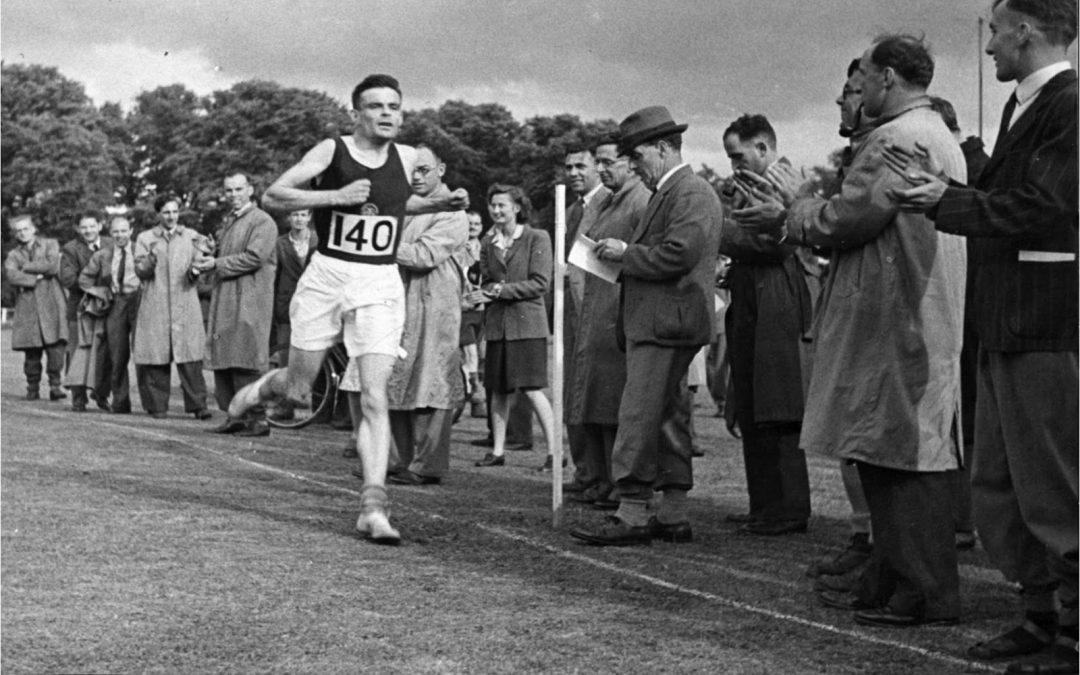
\includegraphics[width=7cm]{ch-turing/img/turing}
\end{center}
\caption*{Alan Turing (1912-1954) était aussi marathonien.}
\end{figure}

Il faut donc imaginer une machine qui peut se déplacer sur un ruban aussi étendu qu'on le désire en avançant ou reculant d'une case à la fois.\\
Définir une machine M c'est se donner
\begin{itemize}
    \item 	un ensemble d'\textit{états} $\mathcal{E}$ dans lesquels la machine M pourra se trouver;
    \item 	un ensemble de \textit{symboles} (un alphabet) $\mathcal{A}$, que la machine peut lire ou écrire sur le ruban;
    \item 	un ensemble de \textit{règles} qui décrivent, selon l'état dans lequel M se trouve et le symbole qu'elle lit, quel symbole elle écrit à
          la place de ce symbole sur le ruban et dans quel sens elle se déplace pour lire le prochain symbole. Cet ensemble de règles peut s'appeler un
          \textit{programme}.
\end{itemize}

\begin{exercice}[]
    Faire l'activité \og Machine de Turing\fg.
\end{exercice}

La machine décrite précédemment ne possède qu'un seul programme. Turing a donc eu l'idée de ce que l'on appelle maintenant une
\textit{Machine de Turing universelle} (MTU).

\begin{figure}[H]
    \begin{center}
        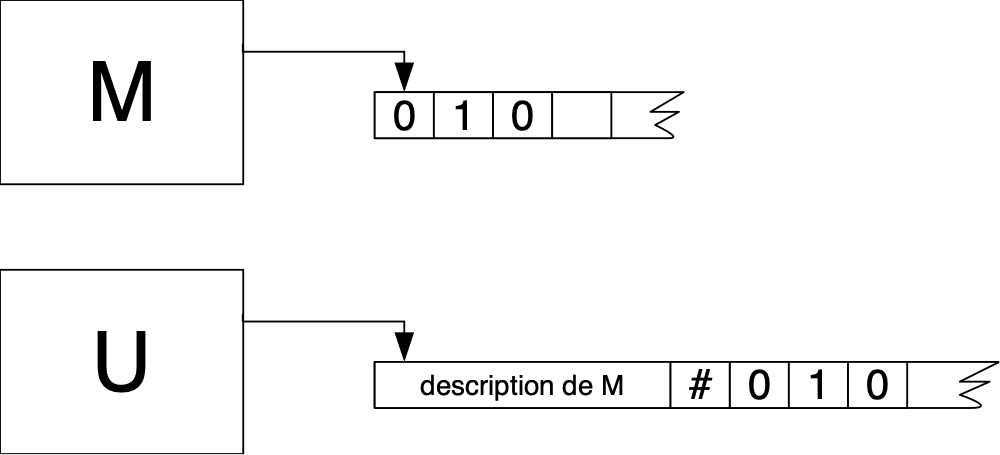
\includegraphics[width=6.5cm]{ch-turing/img/mtu.png}
    \end{center}
    \caption*{Une machine de Truing universelle.}
\end{figure}

Il s'agit d'une machine de Turing U qui est capable de simuler n'importe quelle machine de Turing M,
pourvu qu'on lui fournisse l'ensemble des règles de M et son état de départ. C'est en quelque sorte l'origine de l'ordinateur
programmable, le programme étant les règles de M, et M étant variable.

\subsection{L'ordinateur programmable}

Au milieu des années 40, John Von Neumann et ses collègues ont mis au point une version concrète de l'ordinateur programmable avec une architecture révolutionnaire pour l'époque, qui reste commune à la plupart des ordinateurs actuels et qui porte le nom d'\textit{architecture de Von Neumann}. Celui-ci a expliqué que l'idée de machine de Turing universelle a directement inspiré le projet.

Parmi les premiers ordinateurs figurent l'ENIAC, ordinateur opérationnel à la fin de l'année 1945 et destiné à effectuer des calculs balistiques. C'est une énorme machine, de 90cm d'épaisseur, 2,40m de haut et ... 30,5m de long, le tout pour un poids de 30 tonnes.

\begin{figure}[H]
    \begin{center}
        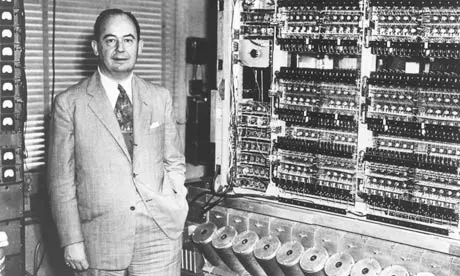
\includegraphics[width=7cm]{ch-turing/img/vonneumann}
    \end{center}
    \caption*{John Von Neumann (1903-1957).}
\end{figure}

Les premières personnes à programmer cet ordinateur sont six femmes, toutes mathématiciennes. L'ordinateur peur réaliser \np{100000} additions par secondes, ou encore 357 multiplications par seconde, ou encore 38 divisions par seconde, le tout avec une capacité mémoire de 20 nombres signés à 10 chiffres en base 10.
\begin{figure}[H]
    \begin{center}
        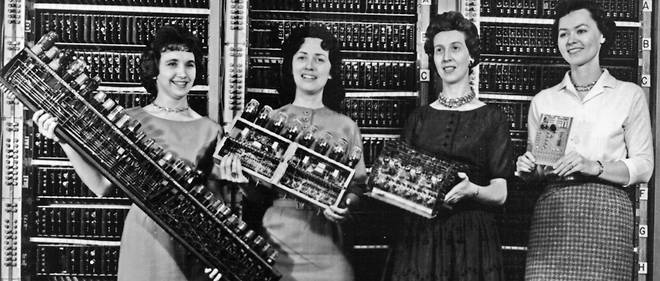
\includegraphics[width=10cm]{ch-turing/img/eniac.jpg}
    \end{center}
    \caption*{Quatre des six programmeuses de l'ENIAC.}
\end{figure}

On peut voir la taille de quelques-uns des \np{17468} tubes à vide qui entraient dans la composition de l'ordinateur. Dès 1947 les transistors ont remplacé les tubes à vides et n'ont cessé d'être miniaturisés. De nos jours les transistors sont directement gravés dans le silicium, leur taille fait quelques nanomètres ($10^{-9}$m) et une carte graphique RTX 2080 en comporte quasiment 20 milliards. La puissance de calcul a beaucoup augmenté puisque le microprocesseur d'un bon PC actuel a une puissance d'environ 150 GFLOPS,  c'est à dire 150 milliards d'opérations sur des nombres en virgule flottante par seconde !

\begin{exercice}[]
    Entre un transistor des années 50 (quelques centimètres) et un transistor actuel, quel est le facteur de réduction de taille ?\\
    Entre l'ENIAC et ses multiplications par seconde et un PC actuel, quel est le facteur d'augmentation de puissance de calcul ?
\end{exercice}

\section{L'architecture de Von Neumann}



Elle décompose l'ordinateur en 4 parties distinctes :
\begin{itemize}
    \item 	l'\textit{unité arithmétique et logique} ou UAL, dont le rôle est d'effectuer des opérations de base;
    \item 	l'\textit{unité de contrôle} et son registre IR, qui est chargée de séquencer les opérations;
    \item 	la \textit{mémoire} qui stocke à la fois les données à utiliser et le programme que l'unité de contrôle va séquencer.
    \item 	les périphériques d'\textit{entrée-sortie} qui permettent de communiquer dans les 2 sens avec l'extérieur.
\end{itemize}

\begin{figure}[H]
    \begin{center}
        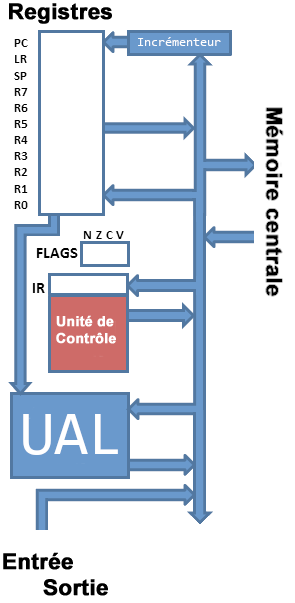
\includegraphics[width=5cm]{ch-turing/img/vn2.png}
    \end{center}
    \caption*{Modèle simplifié de \textit{microprocesseur} (CPU : \textit{Central Processing Unit}).
        Les données transitent par des bus (flèches bleues).}
\end{figure}



Dans le CPU se trouvent des registres :
\begin{itemize}
    \item 	PC (\textit{Program Counter}) qui indique à l'unité de contrôle où aller chercher la prochaine instruction;
    \item 	LR	(\textit{Link Register}) qui contient l'adresse à laquelle le programme doit revenir dans le cas où on aurait appelé un sous-programme (l'équivalent d'une fonction);
    \item 	SP (\textit{Stack Pointer} qui contient l'adresse du sommet de la pile (la pile est un endroit de la mémoire où l'on \og empile\fg{} et \og dépile\fg{} des données, comme une pile d'assiettes);
\end{itemize}
Certaines opérations déclenchent des \og événements\fg{} : quand un résultat est nul, le \textit{flag} (drapeau) Z est mis à un, \textit{et c\ae tera}.

Un processeur donné est capable d'exécuter un nombre d'instructions de base relativement limité. L'ensemble de ces instructions est appelé \textit{langage machine}. Chaque instruction machine est composé d'une ou deux parties :
\begin{itemize}
    \item 	un code opération (appelé \textit{opcode}) qui indique le type de traitement à réaliser ;
    \item 	les données éventuelles sur lesquelles l'opération doit être réalisée.
\end{itemize}

Le fonctionnement d'un CPU est cyclique, la fréquence des cycles étant réglée par une horloge (par exemple un processeur moderne cadencé à 3GHz effectue 3 milliards de cycles par seconde).

\subsection*{Déroulement d'un cycle}

\begin{itemize}
    \item 	le contenu de la RAM pointé par PC est copié dans l'IR de l'unité de contrôle ;
    \item 	l'unité de contrôle décode l'instruction qu'on lui donne et la fait exécuter ;
    \item 	l'exécution provoque l'utilisation des registres, et/ou une lecture ou écriture dans la RAM, éventuellement un accès aux entrées/sorties.
\end{itemize}

Les instructions machine étant \og désespérément austères\fg{} lorsqu'on les écrit en binaire ou en hexadécimal, on les écrit dans un langage compréhensible par les humains. Ce langage s'appelle l'\textit{assembleur}.

\begin{exercice}[]
    Faire l'activité : Simulateur de CPU.
\end{exercice}
% \chapter{Logique}
\section{Du transistor à l'ordinateur}
\arrayrulecolor{white}
Le transistor est à la base de la plupart des composants d'un ordinateur. Pour faire simple c'est un composant avec une entrée, une sortie, et une alimentation.Quand il est alimenté, le transistor laisse passer le courant de l'entrée vers la sortie et dans le cas contraire le courant ne passe pas.\\
C'est l'élément de base des \textit{circuits logiques}.
\begin{definition}[ : circuit logique]
    Un circuit logique prend en entrée un ou plusieurs signaux électriques. Chacun de ses signaux peut être dans l'état 0 ou l'état 1.\\
    En sortie, le circuit logique produit un signal (0 ou 1) obtenu en appliquant des \textit{opérations booléennes} aux signaux d'entrée.
\end{definition}

Un circuit logique est une implémentation matérielle d'une \textit{fonction logique}. La fonction logique est, quant à elle, la version \og mathématique\fg{} du circuit. Nous confondrons ces deux notions par la suite.

\subsection{Opérateurs logiques de base}

À l'aide des opérateurs suivants, on peut construire toutes les fonctions logiques.

\subsubsection*{L'opérateur \og non\fg{}}

C'est un opérateur \textbf{unaire} : il ne prend qu'une seule variable booléenne en entrée.
\tabularstyled
\begin{figure}[H]
    \begin{center}
        \begin{tabular}{|c|c|}
            \hline\rowcolor{UGLiOrange}
            {\boxfont\color{white}x} & {\boxfont\color{white}\textit{non} x} \\
            \hline
            0                        & 1                                     \\
            \hline
            1                        & 0                                     \\
            \hline
        \end{tabular}
        \hspace{3em}
        \tikz{\draw (0,0) node[european not port]{};}
    \end{center}
    \caption*{La table de vérité et le symbole de porte européen du \texttt{non}.}
\end{figure}



Cet opérateur renvoie \og le contraire de ce qu'il a reçu\fg{}.\\
Parmi les notations que l'on rencontre pour noter \og non x\fg{} il y a
\begin{itemize}
    \item 	 \texttt{NOT x}
    \item 	$\barmin{x}$
    \item 	\texttt{!x}
\end{itemize}


\subsubsection*{L'opérateur \og et\fg{}}

C'est un opérateur \textbf{binaire} : il prend deux variables booléennes en entrée.

\begin{figure}[H]
    \begin{center}
        \begin{tabular}{|c|c|c|}
            \hline\rowcolor{UGLiOrange}
            {\boxfont\color{white}x} & {\boxfont\color{white}y} & {\boxfont\color{white}x\textit{et} y} \\
            \hline
            0                        & 0                        & 0                                     \\
            \hline
            0                        & 1                        & 0                                     \\
            \hline
            1                        & 0                        & 0                                     \\
            \hline
            1                        & 1                        & 1                                     \\
            \hline
        \end{tabular}
        \hspace{3em}
        \tikz{\draw (0,0) node[european and port]{};}
    \end{center}
    \caption*{La table de vérité et le symbole de porte européen du \texttt{et}.}
\end{figure}
Un \og et\fg{} ne renvoie vrai que si ses deux entrées sont vraies.\\
Parmi les notations que l'on rencontre pour noter \og x et y\fg{} il y a
\begin{itemize}
    \item 	 \texttt{x AND y}
    \item 	$x\wedge y$
    \item 	\texttt{x \&\& y}
\end{itemize}


\subsubsection*{L'opérateur \og ou\fg{}}

C'est également un opérateur \textbf{binaire}.

\begin{figure}[H]
    \begin{center}
        \begin{tabular}{|c|c|c|}
            \hline\rowcolor{UGLiOrange}
            {\boxfont\color{white}x} & {\boxfont\color{white}y} & {\boxfont\color{white}x\textit{ou} y} \\

            \hline
            0                        & 0                        & 0                                     \\
            \hline
            0                        & 1                        & 1                                     \\
            \hline
            1                        & 0                        & 1                                     \\
            \hline
            1                        & 1                        & 1                                     \\
            \hline
        \end{tabular}\hspace{3em}
        \tikz{\draw (0,0) node[european or port]{};}
    \end{center}
    \caption*{La table de vérité et le symbole de porte européen du \texttt{ou}.}
\end{figure}

Un \og ou\fg{} ne renvoie faux que si ses deux entrées sont fausses.\\
Parmi les notations que l'on rencontre pour noter \og x ou y\fg{} il y a
\begin{itemize}
    \item 	 \texttt{x OR y}
    \item 	$x\vee y$
    \item 	\texttt{x || y}
\end{itemize}

On peut montrer qu'il est possible de se passer de la fonction \textit{et} et que toutes les fonctions logiques peuvent s'écrire à l'aide de
fonctions \textit{non} et \textit{ou} (on peut même n'utiliser qu'une seule fonction : la fonction \og non ou\fg{}). Le choix de ces trois fonctions
\textit{et}, \textit{ou} et \textit{non} est donc, en quelque sorte, arbitraire.

\begin{definition}[ : \'Equivalence de deux circuits/fonctions logiques]
    On dira que deux fonctions logiques sont équivalentes lorsqu'elles prennent le même nombre de variables en entrée (le même nombre de signaux si on parle de circuits) et si ces deux fonctions donnent le même résultat lorsque les variables d'entrées ont les mêmes valeurs : on dit que les fonctions ont même \textit{table de vérité}.
    Lorsque deux fonctions logiques sont équivalentes, on dit aussi que leurs expressions booléennes sont équivalentes.
\end{definition}

\begin{exemple}[s]
    \begin{itemize}
        \item 		Les expressions booléennes not(A and B) et (not A) or (not B) sont équivalentes.\\
              Pour le prouver il suffit de vérifier que leurs tables de vérité sont les mêmes : on fait varier les valeurs de A et de B selon toutes les possibilités et on regarde le résultat de chaque expression.
              \begin{center}
                  \begin{tabular}{|c|c|c|c|}
                      \hline\rowcolor{UGLiOrange}
                      {\boxfont\color{white}
                      A} & {\boxfont\color{white}B} & {\boxfont\color{white}A and B} & {\boxfont\color{white}not (A and B)} \\
                      \hline
                      0  & 0                        & 0                              & \cellcolor{UGLiOrange!25}	1          \\
                      \hline
                      0  & 1                        & 0                              & \cellcolor{UGLiOrange!25}	1          \\
                      \hline
                      1  & 0                        & 0                              & \cellcolor{UGLiOrange!25}	1          \\
                      \hline
                      1  & 1                        & 1                              & \cellcolor{UGLiOrange!25}	0          \\
                      \hline
                  \end{tabular}\\[2em]

                  \begin{tabular}{|c|c|c|c|c|}
                      \hline\rowcolor{UGLiOrange}
                      {\boxfont\color{white}A} & {\boxfont\color{white}B} & {\boxfont\color{white}not A} & {\boxfont\color{white}not B} & {\boxfont\color{white}(not A) or (not B)} \\
                      \hline
                      0                        & 0                        & 1                            & 1                            & \cellcolor{UGLiOrange!25}	1               \\
                      \hline
                      0                        & 1                        & 1                            & 0                            & \cellcolor{UGLiOrange!25}	1               \\
                      \hline
                      1                        & 0                        & 0                            & 1                            & \cellcolor{UGLiOrange!25}	1               \\
                      \hline
                      1                        & 1                        & 0                            & 0                            & \cellcolor{UGLiOrange!25}  0              \\
                      \hline
                  \end{tabular}
              \end{center}
              Les dernières colonnes de chaque tableau sont les mêmes : les expressions sont donc équivalentes.
        \item 	En procédant de même on montre très facilement que \og non non x\fg{} et \og x\fg{} sont équivalentes.
    \end{itemize}
\end{exemple}

\begin{exercice}[]
    Montrer que  not(A or B) et (not A) and (not B) sont équivalentes.\\
\end{exercice}

\begin{exercice}[]
    On peut définir le \og ou exclusif\fg{} noté xor comme ceci :  A xor B n'est vrai que si A est vrai ou B est vrai, mais pas les deux.
    \begin{enumerate}
        \item 	Donner la table de vérité de xor.
        \item 	Montrer que A xor B équivaut à (A or B) and (not(A and B)).
        \item 	Montrer que A xor B équivaut à (A and (not B) ) or ( (not A) and B).
        \item 	Représenter A xor B avec un circuit logique, en utilisant les symboles de porte logique européens.
    \end{enumerate}
\end{exercice}

\begin{exercice}[]
    On définit l'opération \og nor\fg{}, notée $\downarrow$ par : $$A\downarrow B = not(A\ or\ B)$$

    Cette opération est dite \textit{universelle} car elle permet de retrouver toutes les autres opérations.

    \begin{enumerate}
        \item 	\'Ecrire la table de vérité de nor.
        \item 	Montrer que $A\downarrow A = not\ A$.
        \item 	En utilisant les exemples de la page précédente, en déduire que $$(A\downarrow B)\downarrow(A\downarrow B) = A\ or\ B$$
        \item 	Comment à partir de A, B et $\downarrow$ obtenir $A\ and\ B$?
    \end{enumerate}
\end{exercice}

\subsection{Un exemple détaillé : le multiplexeur}

Il s'agit d'une fonction très importante : soient A, B et C trois variables logiques, alors m(A,B,C)=B si A vaut 0 et C si A vaut 1.\\ m permet
donc de sélectionner B ou C suivant la valeur de A. Voici la table de valeurs de m :
\begin{center}
    \begin{tabular}{|c|c|c|c|}
        \hline\rowcolor{UGLiOrange}
        {\boxfont\color{white}A} & {\boxfont\color{white}B} & {\boxfont\color{white}C} & {\boxfont\color{white}m(A,B,C)} \\
        \hline
        0                        & 0                        & 0                        & 0                               \\
        \hline
        0                        & 0                        & 1                        & 0                               \\
        \hline
        0                        & 1                        & 0                        & 1                               \\
        \hline
        0                        & 1                        & 1                        & 1                               \\
        \hline
        1                        & 0                        & 0                        & 0                               \\
        \hline
        1                        & 0                        & 1                        & 1                               \\
        \hline
        1                        & 1                        & 0                        & 0                               \\
        \hline
        1                        & 1                        & 1                        & 1                               \\
        \hline
    \end{tabular}
\end{center}

On va décomposer m à l'aide des opérateurs de base. Ici, un raisonnement simple permet d'y arriver :
\begin{itemize}
    \item quand A vaut 0, on peut garder la valeur de B en faisant (\textit{non} A) \textit{et} B;
    \item quand A vaut 1, on peut garder la valeur de C en faisant A \textit{et} C;
    \item il se trouve que ces deux observations vont bien ensemble car quand A vaut 0, A \textit{et} C vaut automatiquement 0, et quand A vaut
          1, (\textit{non} A) \textit{et} B vaut automatiquement 0;
    \item on en conclut que l'\textbf{expression symbolique} de m est
          \begin{center}
              m(A,B,C) =  (A \textit{et} C) ou ((\textit{non} A)  \textit{et} B).
          \end{center}
\end{itemize}
Le circuit logique modélisant m est le suivant :
\begin{center}
    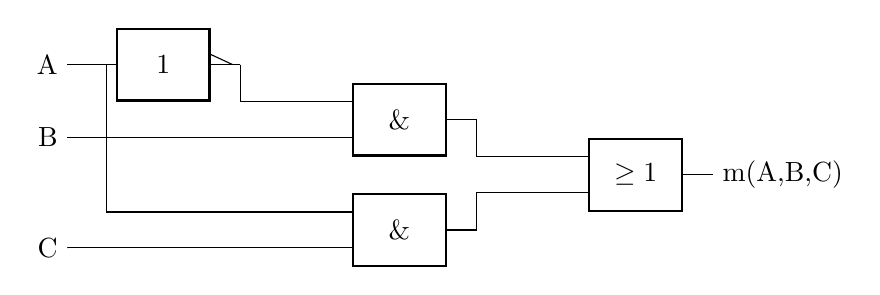
\begin{tikzpicture}[yscale=.7]
        \coordinate (A) at (0,4);
        \draw (A) node[left]{A}	 ;
        \coordinate (B) at (0,2.68);
        \draw (B) node[left]{B}	 ;
        \coordinate (C) at (0,.68);
        \draw (C) node[left]{C}	 ;
        \node[european not port] (not1) at (2,4) {};
        \node[european and port] (and1) at (5,3) {};
        \node[european and port] (and2) at (5,1) {};
        \node[european or port] (or1) at (8,2) {};
        \draw (and1.out) |- (or1.in 1) (and2.out) |- (or1.in 2);
        \draw (C) |- (and2.in 2);
        \draw (B) |- (and1.in 2);
        \draw (not1.out) |- (and1.in 1);
        \draw (A) |- (not1.in);
        \draw (0.5,4)|- (and2.in 1);
        \draw (or1.out)  node[right]{m(A,B,C)};
    \end{tikzpicture}
\end{center}

\begin{exercice}[]
    On veut construire un \og additionneur\fg{} selon le principe suivant :
    \begin{itemize}
        \item 	A et B représentent deux bits à ajouter
        \item 	S et R sont respectivement
              \begin{itemize}
                  \item 	la somme (sur un bit, donc) de A et B;
                  \item 	la retenue.
              \end{itemize}
    \end{itemize}
    Par exemple si A et B valent 1, alors S vaudra 0 et R vaudra 1.
    \begin{enumerate}
        \item 	Donner les tables de vérités de R et de S.
        \item 	Exprimer R et S en fonction de A et B et des opérations \og non\fg{}, \og ou\fg{} et \og et\fg{}.
        \item 	Représenter R et S avec un (ou des) circuit(s) logique(s), en utilisant les symboles de porte logique européens.
    \end{enumerate}
\end{exercice}

\begin{exercice}
    Pour chiffrer un message, une méthode, dite du masque jetable, consiste à le combiner avec une chaîne de caractères de longueur comparable.
    Une implémentation possible utilise l’opérateur \texttt{XOR} (ou exclusif) dont voici la table de vérité :
    \begin{center}
        \begin{tabular}{|c|c|c|}
            \hline
            \rowcolor{UGLiOrange} {\boxfont\color{white}a} & {\boxfont\color{white}b} & {\boxfont\color{white}a XOR b} \\
            \hline
            0                                              & 0                        & 0                              \\
            \hline
            0                                              & 1                        & 1                              \\
            \hline
            1                                              & 0                        & 1                              \\
            \hline
            1                                              & 1                        & 0                              \\
            \hline
        \end{tabular}
    \end{center}
    Dans la suite, les nombres écrits en binaire seront précédés du préfixe \texttt{0b}.
    \begin{enumerate}
        \item Pour chiffrer un message, on convertit chacun de ses caractères en binaire (à l’aide du format \textsc{Unicode}), et on réalise l’opération \texttt{XOR} bit à bit avec la clé.\\

              Après conversion en binaire, et avant que l’opération XOR bit à bit avec la clé n’ait été effectuée, Alice obtient le message suivant :

              \begin{center}
                  \texttt{m = 0b 0110 0011 0100 0110}
              \end{center}
              \begin{enumalph}
                  \item 	Le message \texttt{m} correspond à deux caractères codés chacun sur 8 bits : déterminer quels sont ces caractères. On fournit pour cela la table ci-dessous qui associe à l’écriture hexadécimale d’un octet le caractère correspondant. \\[.5em]
                        \begin{center}
                            \includegraphics[width=10cm]{ch-logique/img/ascii}\\
                        \end{center}
                        \textit{\footnotesize Exemple de lecture : le caractère correspondant à l’octet codé \texttt{4A} en hexadécimal est la lettre \texttt{J}.}\\
                  \item Pour chiffrer le message d’Alice, on réalise l’opération \texttt{XOR} bit à bit avec la clé suivante :
                        \begin{center}
                            \texttt{k = 0b 1110 1110 1111 0000}
                        \end{center}
                        Donner l’écriture binaire du message obtenu.
              \end{enumalph}

        \item 	\begin{enumalph}
                  \item 	Donner la table de vérité de l'expression booléenne \texttt{(a XOR b) XOR b}.
                  \item 	Bob connaît la chaîne de caractères utilisée par Alice pour chiffrer le message. Quelle opération doit-il réaliser pour déchiffrer son message?
              \end{enumalph}
    \end{enumerate}
\end{exercice}
% \chapter{Systèmes d'exploitation}

	\section{Qu'est-ce qu'un système d'exploitation ?}
	
	\floatpictureright{0.2}{ch-sysex/img/sysex.png}{
		Un système d'exploitation (\textit{Operating System} en anglais, abrégé OS) est un ensemble de programmes. Il a plusieurs fonctions :
		\begin{itemize}
			\item 	c'est un intermédiaire entre l'utilisateur et les applications qu'il utilise (qui sont aussi des programmes) et le matériel ;
			\item 	c'est lui qui partage les \textit{ressources} entre les différents programmes en train d'être exécutés voire entre les différents utilisateurs ;
			\item 	c'est lui qui protège la machine des applications, et les applications les unes des autres ;
			\item 	c'est lui qui gère l'adaptation entre l'\textit{interface} (graphique par exemple) et le matériel.
		\end{itemize}
	}\medskip\par
	Les ressources, ce sont entre autres : 
	\begin{itemize}
		\item 	le matériel qui compose l'ordinateur proprement dit (CPU, mémoire, carte graphique...) et les \textit{périphériques} (imprimante, clé usb, clavier) ;
		\item 	les fichiers ;
		\item 	les éventuelles connexions à des réseaux.
	\end{itemize}
	\floatpictureleft{0.5}
	{ch-sysex/img/oss.png}
	{
		Il existe de multiples OS.
		\begin{itemize}
			\item 	pour PC : \textsc{Windows} et beaucoup de distributions de \textsc{Linux} ;
			\item 	pour \textsc{Apple} : \textsc{MacOS} ;
			\item	pour iPhone et iPad : \textsc{iOS} ;
			\item 	pour beaucoup de smartphones : \textsc{Android}.
		\end{itemize}}\medskip\par
	
%---------------

	Les appareils connectés ainsi que les « box »  des fournisseurs d'accès à Internet et les consoles de jeux disposent aussi de leurs OS.
	Certains OS sont \textit{gratuits}, d'autres \textit{payants}.
	
	\section{Le système de gestion des fichiers}
	
	Un \textit{fichier} est un ensemble de données numériques réunies sous un même nom et enregistré sur un support de mémoire permanent appelé \textit{mémoire de masse} (ce peut être un disque dur, un DVD-rom, une clé USB, une carte SD).\\
	Un \textit{système de gestion de fichiers} est une façon de stocker les fichiers sur la mémoire de masse. La plupart des systèmes d'exploitation stockent les fichiers dans des \textit{répertoires} organisés de manière hiérarchique selon une \textit{arborescence} (voir plus bas).

	\section{L'exemple de Linux et du shell}

	\floatpicturerightcaption{0.5}{ch-sysex/img/pi4.jpg}{les Raspberry Pi tournent sous Linux}{
		En 1970 nait \textsc{UNIX}, l'un des premiers système d'exploitation multi-utilisateurs.\\
		Cependant ce système d'exploitation n'est pas \textit{libre}, c'est à dire que son code source n'est pas à la disposition du public.\\
		En 1991, un étudiant finlandais du nom de Linus Torvalds entreprend de créer un clone d'\textsc{UNIX} en le réécrivant totalement.
	}\medskip\par
	Ce nouveau système d'exploitation libre s'appelle \textsc{Linux} et est désormais largement utilisé.\\
	C'est la plupart du temps une version (appelée \textit{distribution}) de \textsc{Linux} que l'on installe sur les ordinateurs Raspberry Pi.
	
	\begin{center}
		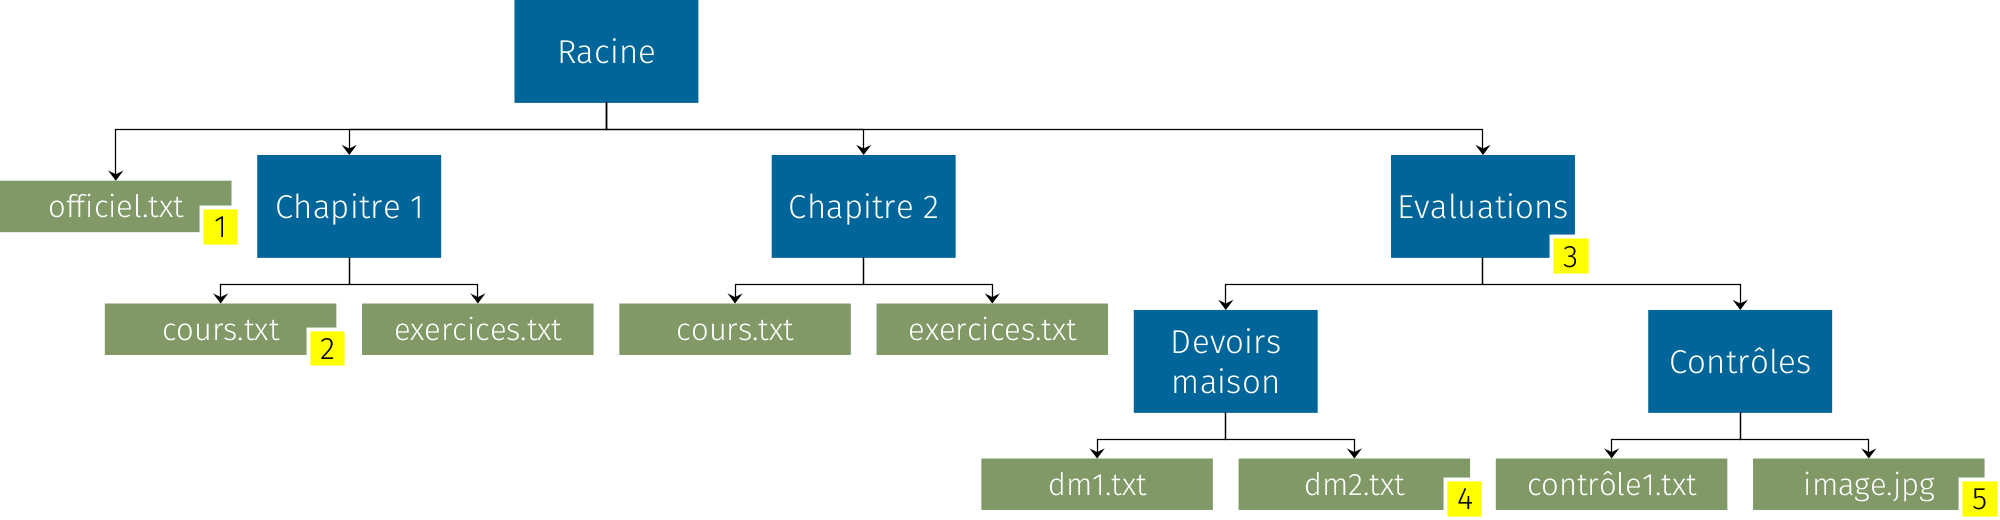
\includegraphics[width=\textwidth]{ch-sysex/img/hier.png}\\
		\footnotesize\textit{Exemple d'arborescence de fichiers.}
	\end{center}

	Dans un système de fichier tel que celui de \textsc{Linux}, la racine se note \texttt{/} et les séparateurs (équivalents des flèches du graphique ci-dessus) aussi.\\
	Il y a deux manières d'accéder aux fichiers.

	\subsubsection{Chemin absolu}
	On part de la racine et on écrit le chemin pour arriver à l'objet désiré.\\
	Ainsi le chemin absolu de l'objet 1 est \texttt{/officiel.txt} et celui de l'objet 5 est \texttt{/Evaluations/Contrôles/image.jpg}
	
	\begin{exercice}[]
		Donner les chemins absolus des autres objets.
	\end{exercice}

	

	\subsubsection{Chemin relatif}
	On part d'un emplacement précis (à l'intérieur d'un répertoire) et l'on indique le chemin pour aller à l'objet voulu. S'il faut remonter d'un cran dans l'arborescence on utilise na notation \texttt{..} comme ceci :
	\begin{itemize}
		\item 	si l'on est dans le répertoire \texttt{Evaluations} et qu'on veut accéder à \texttt{dm2.txt} alors son chemin relatif est \texttt{Devoirs maison/dm2.txt};
		\item 	si l'on est dans \texttt{Contrôles} et qu'on veut accéder au exercices du chapitre 1, le chemin relatif est \texttt{../../Chapitre 1/exercices.txt} car il faut d'abord remonter l'arborescence de 2 crans.
	\end{itemize}

	\begin{exercice}[]
		On est dans le répertoire \texttt{Contrôles}, donner les chemins relatifs des objets 1 à 5.
	\end{exercice}
	
	\subsection{Le shell}
	
	Nous sommes habitués à un environnement graphique pour gérer les copies et déplacements de nos dossiers (et bien d'autre choses comme par exemple sélectionner des fichiers à compresser) mais ce n'est pas la seule manière. Dans tout système d'exploitation muni d'un environnement graphique, on peut trouver un \textit{terminal} (aussi appelé \textit{invite de commande}, ou \textit{shell}) parce que
	\begin{itemize}
		\item 	c'est avec cette interface textuelle minimaliste que l'on interagissait avec l'\textsc{OS} avant;
		\item 	finalement quand on sait (très bien) s'en servir, on peut faire beaucoup plus de choses plus rapidement avec un shell et au clavier qu'avec un clavier, une souris et un environnement graphique.
	\end{itemize}

	\begin{exercice}[]
		Faire l'activité \textit{utiliser le shell}.
	\end{exercice}
	
% \chapter{Unité et diversité des langages}

\section{Des éléments communs}
Un langage de programmation sert à traduire des algorithmes pour les exécuter sur un ordinateur. Il est composé 
\begin{itemize}
    \item   d'un alphabet (ensemble de lettres et de symboles);
    \item   d'un vocabulaire (les \textit{mots-clés} du langage);
    \item   d'une grammaire (la \textit{syntaxe} du langage).
\end{itemize}

Les notions suivantes sont communes à l'immense majorité des langages :

\begin{itemize}
    \item   une \textit{instruction} est un ordre donné;
    \item   une \textit{variable} est un nom qui fait référence à une donnée manipulée par le programme et susceptible de changer au cours de celui-ci;
    \item   une \textit{constante} est un nom qui fait référence à une valeur immuable;
    \item   un \textit{type} qui sert à classifier une variable ou une constante et conditionne les opérations qu'il est possible d'effectuer;
    \item   la \textit{déclaration} consiste à renseigner le traducteur du programme sur la nature des données du programme (type, valeur).
    \item   les \textit{structures de contrôle} telles que le \textit{test} et les \textit{boucles}.
    \item   une \textit{fonction} (ou procédure, ou méthode) sert à isoler un fragment de programme pour pouvoir l'utiliser (éventuellement plusieurs fois) de manière paramétrée.
\end{itemize}

\section{Des différences}

\subsection{Différences formelles}

Tous les langages n'utilisent pas la même syntaxe. En examinant un même algorithme écrit dans plusieurs langages, on constate que 

\begin{itemize}
    \item   L'affectation peut être signifiée par \texttt{=} (comme en \textsc{Python}, \textsc{Basic}, \textsc{C}, \textsc{Fortran}...) ou par \texttt{:=} (\textsc{Ada}, \textsc{Algol}, \textsc{Go} pour partie...). On utilise aussi \texttt{<-} en \textsc{Caml}.
    \item   Les \textit{listes} (ou tableaux) sont très souvent indicées à partir de zéro... Mais pas toujours (\textsc{Fortran}, \textsc{Lua}).
    \item   Très souvent, les structures de contrôles sont délimitées par des accolades (\textsc{C}, \textsc{Java},  \textsc{Kotlin}...) ou par des \texttt{begin} et des \texttt{end} (\textsc{Ruby}, \textsc{Pascal}...). Parfois on utilise des variantes du \texttt{end} telles que \texttt{done}, \texttt{END-IF} ou \texttt{NEXT} pour signifier une fin de boucle « pour» .
\end{itemize}

Certains langages ont des syntaxes très similaires : le langage \textsc{C}, \textsc{Java} et \textsc{Javascript} par exemple (notamment le fait qu'un point-virgule termine une ligne).\\
D'autres ont une syntaxe et une mise en forme particulière, éloignée de tous les autres, comme le \textsc{Basic} ou le \textsc{Cobol}.

\subsection{Différences structurelles}

Certains langages obligent à déclarer le type des variables lors de leur création. C'est le cas de \textsc{C} ou \textsc{Java}. D'autres obligent même à renseigner les variables et leur type avant toute chose, comme \textsc{Ada}, \textsc{Algol}, \textsc{Cobol}. Ce n'est pas le cas en \textsc{Python} ou en \textsc{Ruby}.\\

Une autre différence majeure vient de la manière dont est traité le programme par le traducteur :

\begin{itemize}
    \item   En \textsc{C} ou en \textsc{C++}, le programme est transformé en \textit{langage-machine} par un \textit{compilateur}. L'intérêt est que l'on gagne en rapidité lors de l'exécution du programme.
    \item   En \textsc{Python} le programme est \textit{interprété}  lors de son exécution, ligne par ligne.
    \item   Beaucoup de langages utilisent un procédé hybride : le langage utilise une machine virtuelle, et les programmes sont compilés dans le langage de cette machine virtuelle, qui sera ensuite exécuté. La compilation peut être faite avant et le résultat stocké dans un fichier, ou bien être faite à la volée (\textit{Just In Time compilation}).
\end{itemize}



Chaque langage suit un ou plusieurs \textit{paradigmes} de programmation qui change radicalement la manière d'écrire les programmes.\\
Chaque langage suit un ou plusieurs \textit{paradigmes} de programmation qui change radicalement la manière d'écrire les programmes.\\
Nous avons vu la programmation \textit{impérative} (séquentielle, linéaire) où le programme effectue une liste d'instructions pas-à-pas. Il existe la programmation \textit{évènementielle} lors de laquelle on précise à \textsc{Processing} ce qu'il doit faire quand tel ou tel évènement se produit.\\
D'autres paradigmes de programmation telle la programmation \textit{orientée objet} ou la programmation \textit{fonctionnelle} sont très utilisés.

Enfin on distinguera des différences dans les contexte d'utilisation de chaque langages : il existe des langages généralistes, des langages qui sont censés être exécutés sur des « serveurs de pages web»  tels \textsc{PHP}, d'autres qui (à la base) ont été conçus pour être exécutés au sein même d'un navigateur (\textsc{Javascript}).

\begin{center}
    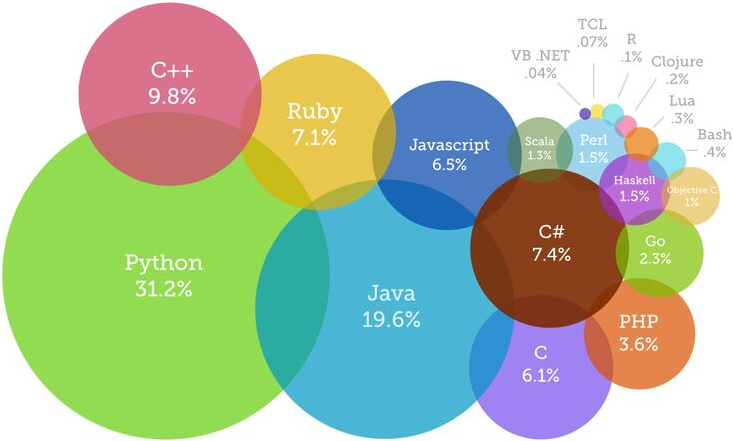
\includegraphics[width=7cm]{ch-langages/img/languages.png}\\ \scriptsize   Langages les plus appris en 2019.\\
    Source : \texttt{learnworthy.net}.
\end{center}
\section{\'Evolution au cours du temps}


Les progrès réalisés sur les analyseurs de code permettent de créer des langages avec une syntaxe de plus en plus épurée courte et pour lesquels il n'est pas obligé de déclarer le type de chaque variable.\\
Les nouveaux langages s'inspirent souvent de leurs prédécesseurs.\\
    
On continue d'inventer de nouveaux langages : ceux-ci sont crées en fonction des besoins de l'époque.\\
De nos jours, les langages qui permettent de programmer facilement plusieurs tâches simultanées (comme par exemple récupérer des données sur \textsc{Internet} et en même temps traiter ces données) ont le vent en poupe.

\begin{center}
    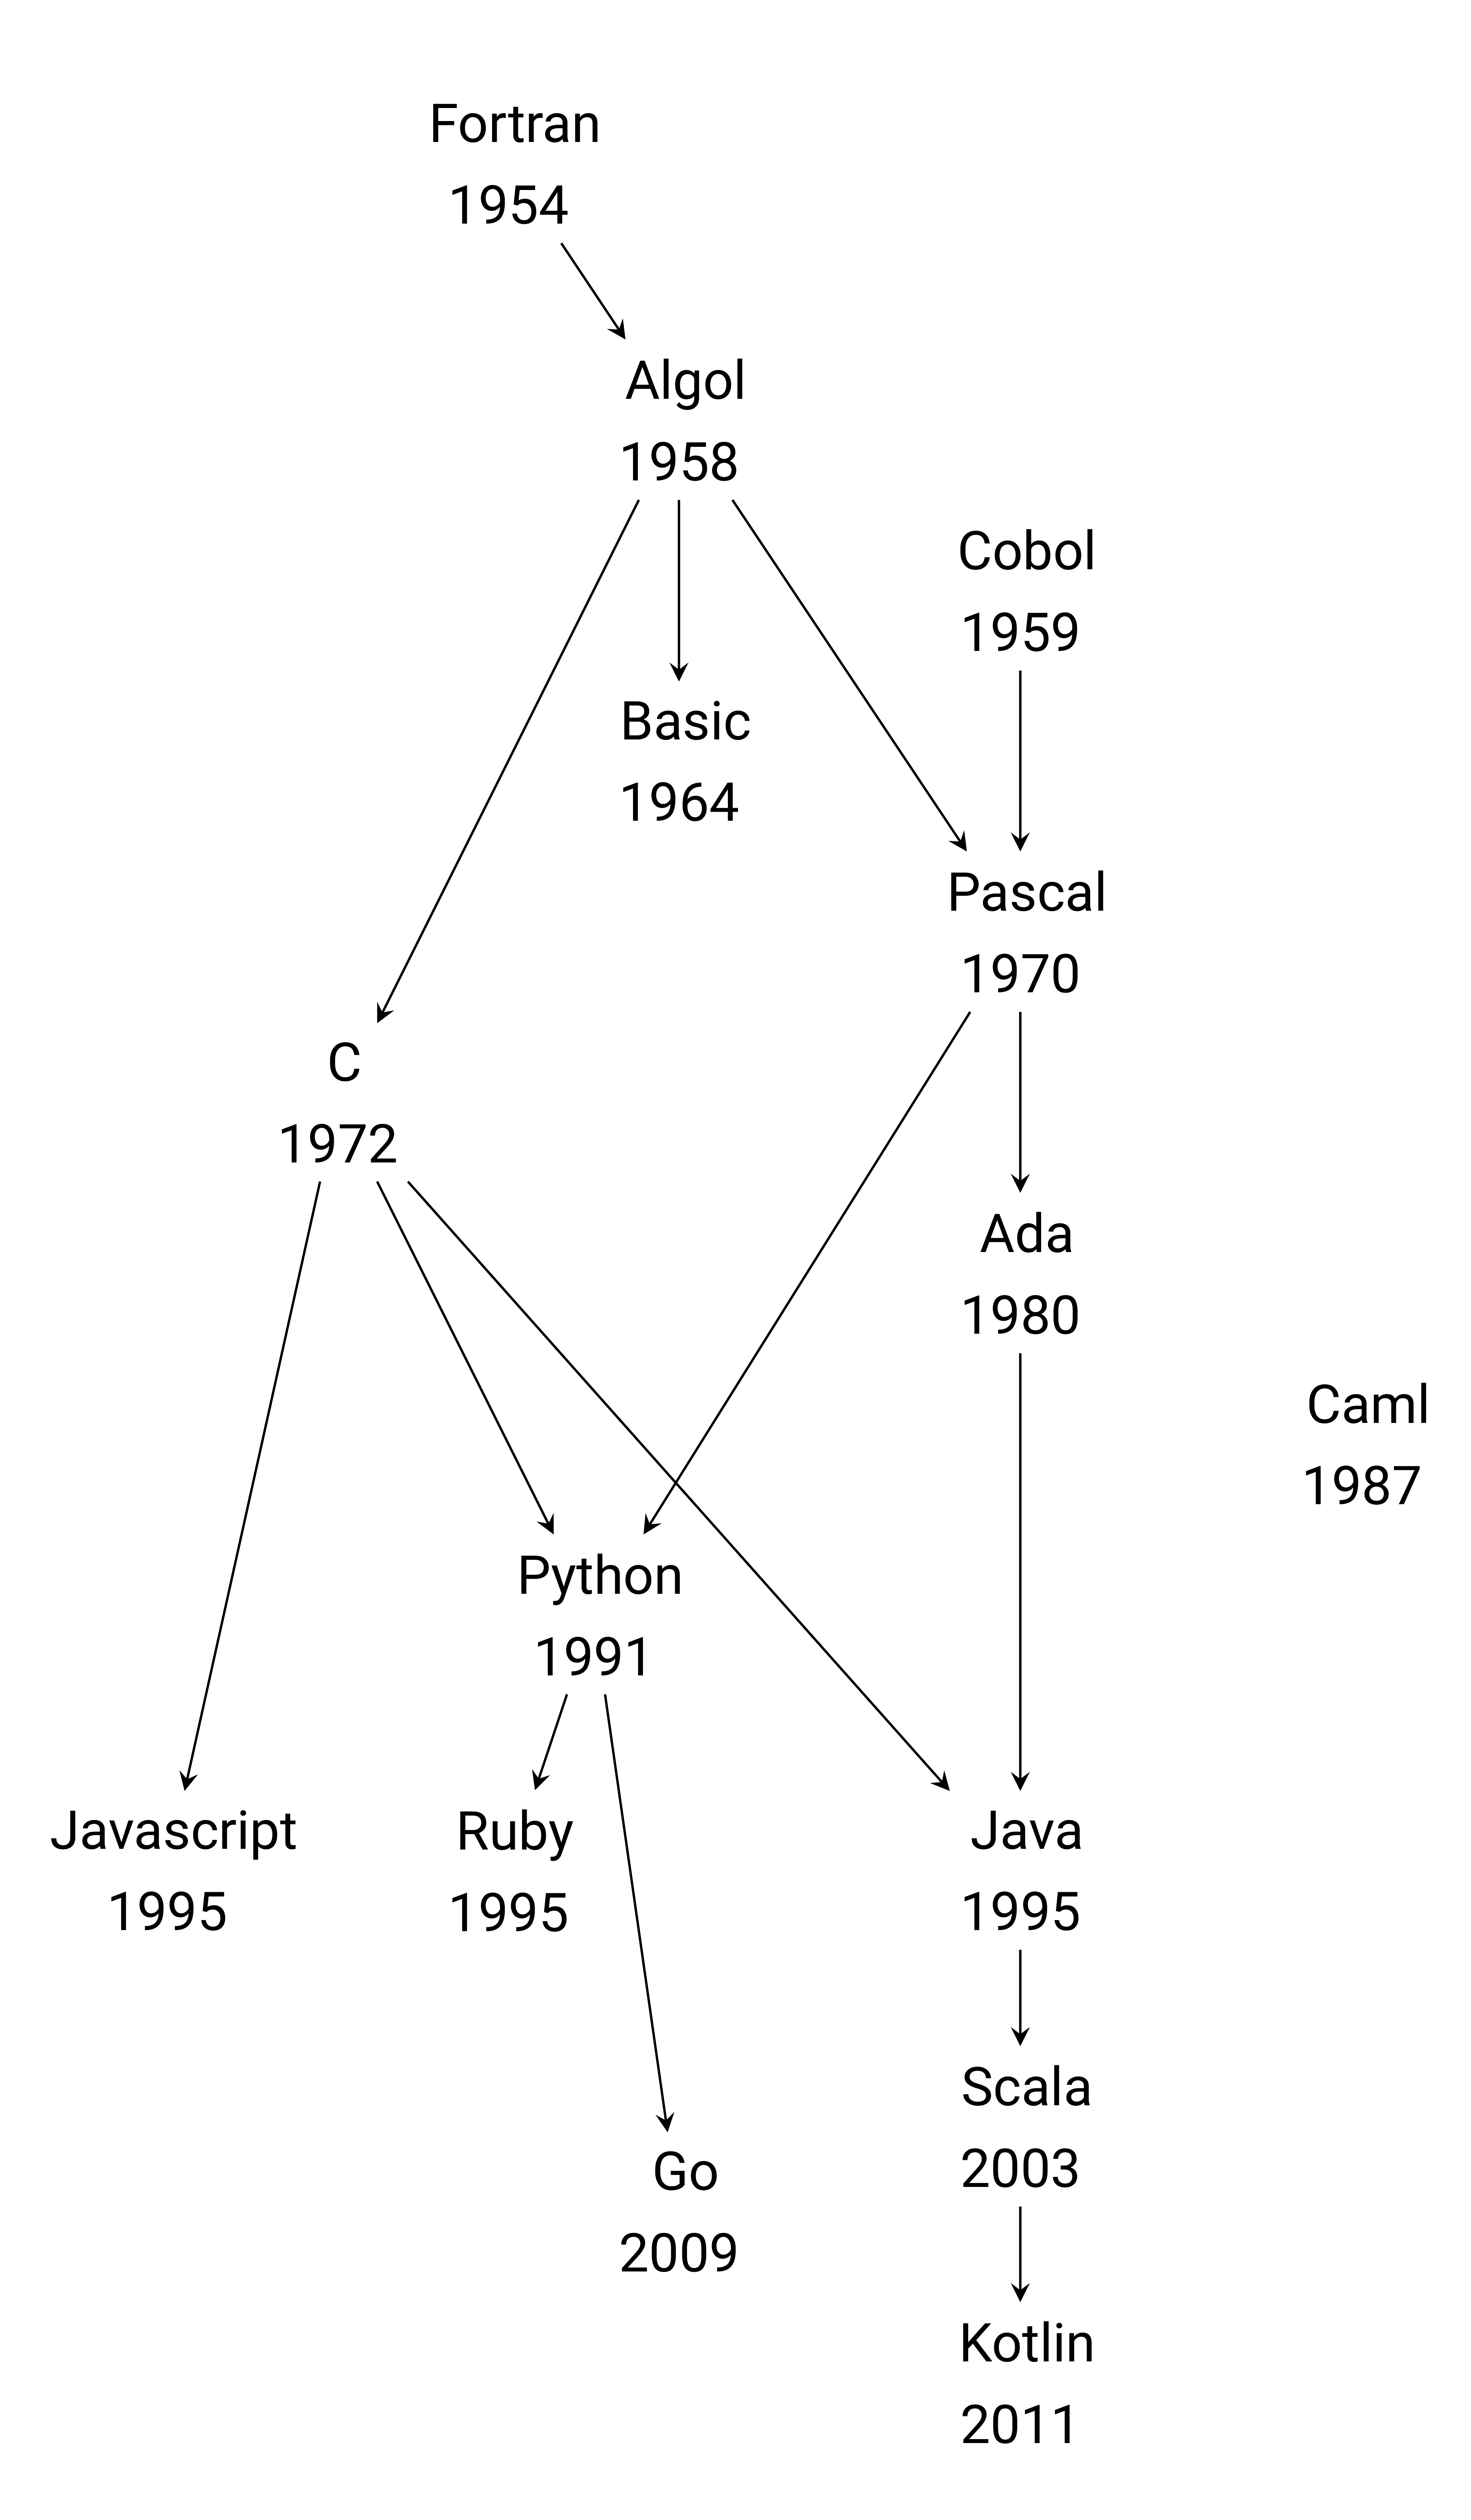
\includegraphics[width=5cm]{ch-langages/img/genealogie.png}\\ \scriptsize   Voici un graphe indiquant comment les langages anciens ont influencé les nouveaux.\\
\end{center}
\ \\[3em]



\begin{center}
    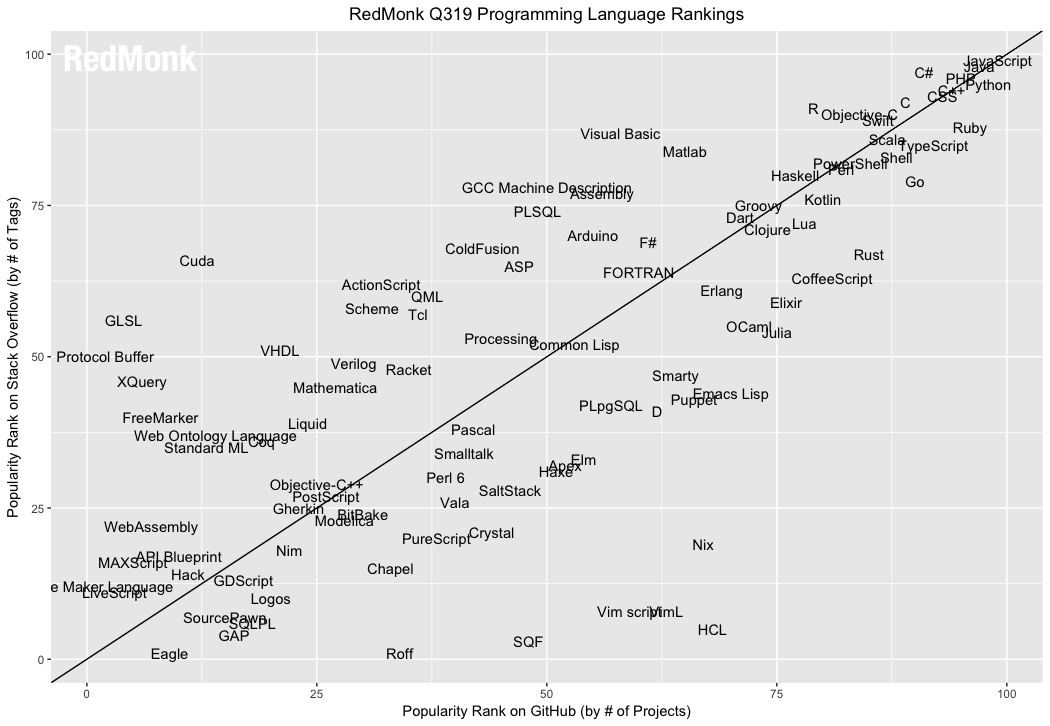
\includegraphics[width=7cm]{ch-langages/img/rank.png}\\ \scriptsize    \textit{Stack Overflow} est un forum d'entraide à la programmation.\\ \textit{GitHub} est un service d'hébergement de projets logiciels.\\
    Le graphique suivant indique la popularité de différents langages sur ces deux sites.\\
    Source : \texttt{redmonk.com}.
\end{center}


% % \part{Réseaux}

%  \chapter{Réseau - principes}

Un \textit{réseau}, c'est un ensemble d'\textit{entités} qui \textit{communiquent} :
\begin{itemize}
    \item 	des fourmis qui envoient des informations par voie \textit{chimique} (les phéromones)  ;
    \item 	des individus qui s'envoient des colis postaux ou du courrier  ;
    \item 	des ordinateurs qui s'envoient des données.
\end{itemize}
Chacun des trois exemples ci-dessus est remarquable par son efficacité.
Le premier est sans doute le fruit de l'évolution.\\
Le deuxième est le résultat de \textit{conventions} et \textit{processus} que les êtres humains ont produits : parmi ces conventions il y a les règles d'écriture d'une adresse postale et aussi le moyen de payer le transport du colis \textit{via} un ou des timbres postaux et parmi les processus il y a l'acheminement du courrier par voie routière, ferrée, maritime ou aériench-reseaux/imgne.\\
Quant au troisième, il est également le fruit de conventions et processus très aboutis que nous allons tenter de détailler dans ce chapitre, il fonctionne remarquablement bien et s'appelle Internet. Ce réseau, composé de \textit{milliards} de machines qui communiquent entre elles et qui permet à deux ordinateurs séparés de milliers de kilomètres de s'échanger une quantité considérable d'informations en une fraction de seconde est bel et bien la plus grande structure que l'être humain ait construit à ce jour. Elle mérite bien qu'on s'attarde un peu sur son fonctionnement.\\

\section{L'idée du modèle à couches empilées}

La finalité d'un réseau, quel qu'il soit, c'est transporter de la manière la plus fiable possible des informations, lesquelles sont émises par une entité A, à destination d'une entité B, et seront transmises en passant très probablement par des entités intermédiaires.\\
Le processus peut être variable mais il existe des mécanismes communs à la plupart des moyens de communication : on cherche à décomposer en étapes et les similitudes apparaissent :
\begin{itemize}
    \item 	A possède une information « brute » ;
    \item 	l'information est « conditionnée » pour être envoyée ;
    \item 	il existe un moyen fiable de savoir comment faire arriver l'information en B ;
    \item 	en définitive, la transmission s'effectue par un moyen physique ;
    \item 	du point de vue de B, les choses s'effectuent « à l'envers » : par moyen physique, A a réussi à lui faire parvenir une information « conditionnée » que B traite pour finalement disposer de l'information brute de A.
\end{itemize}

\subsection{L'exemple du réseau postal}
Les considérations précédentes sont très abstraites, nous allons donc envisager l'exemple d'une personne A qui souhaite envoyer un cadeau à B. L'information est le cadeau en lui même, le réseau est le réseau postal :
\begin{center}
    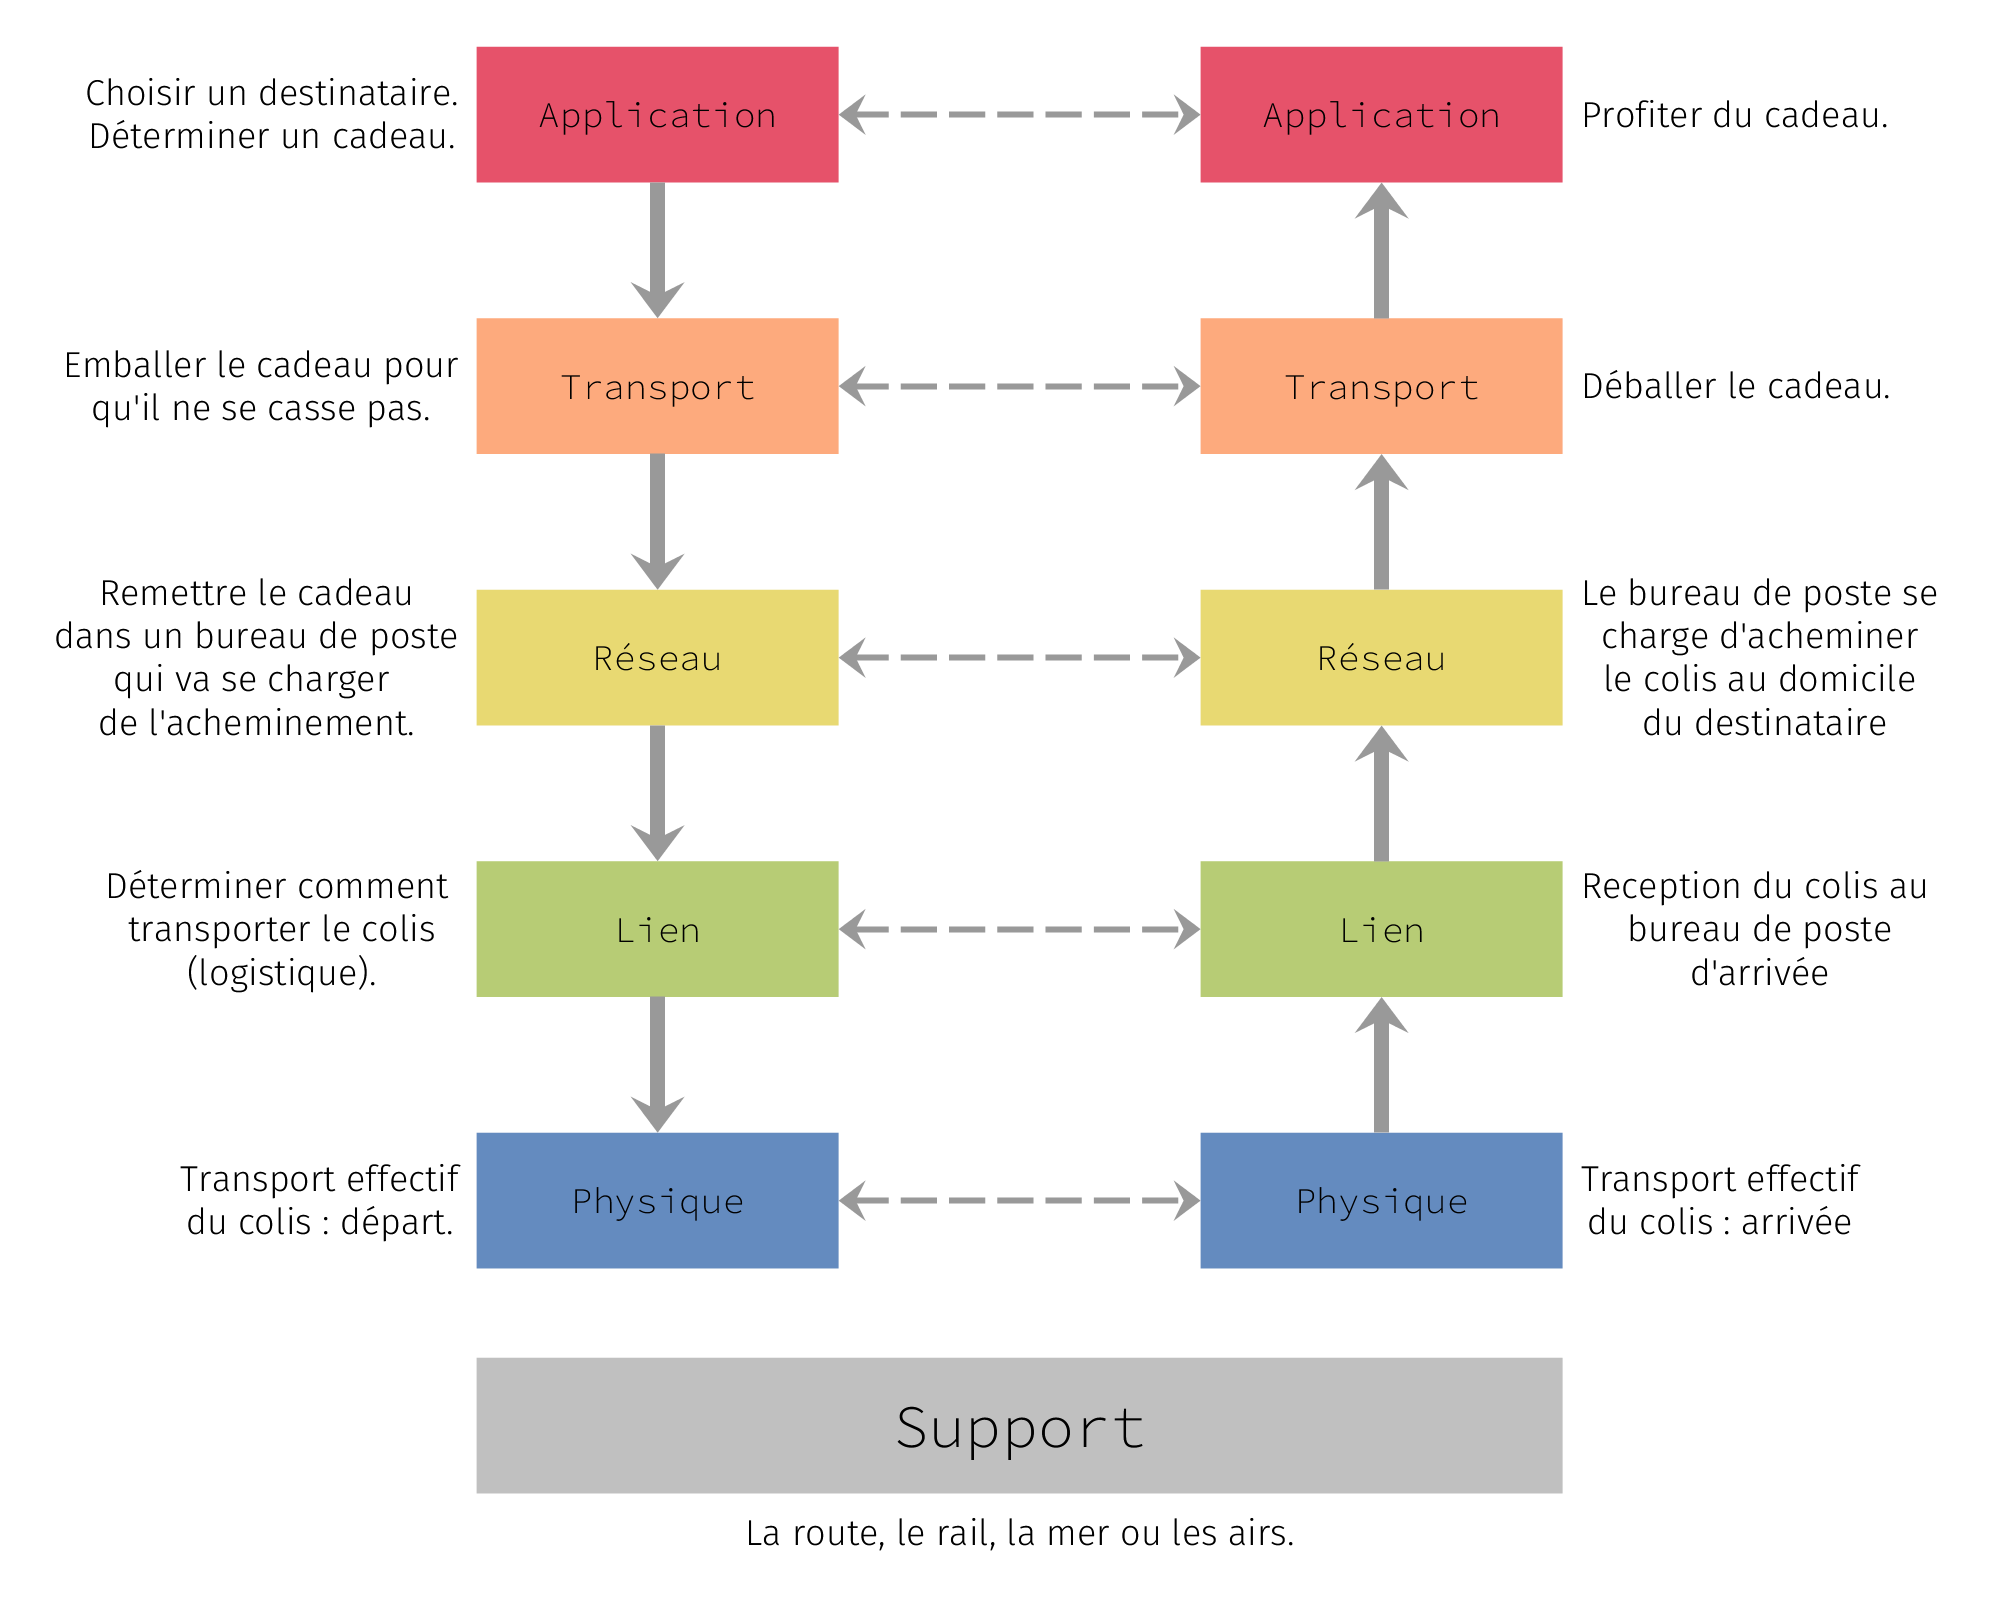
\includegraphics[width=\textwidth]{ch-reseaux/img/modele_5_couches_poste.png}
\end{center}
On a décomposé la communication en 5 couches, auxquelles on a donné des noms \textit{qui sont déjà liés au vocabulaire des réseaux informatiques}. En voici le détail dans l'ordre chronologique:
\begin{itemize}
    \item 	\textbf{Du point de vue de A :}
          \begin{itemize}
              \item 	\textbf{Couche 5 - Application : } A veut envoyer un cadeau à B ;
              \item 	\textbf{Couche 4 - Transport :} le cadeau est emballé pour pouvoir être transporté et reçu intact. On y met aussi l'adresse postale de B ;
              \item 	\textbf{Couche 3 - Réseau :} le bureau  de poste détermine comment acheminer le colis : il a déjà l'adresse postale de B mais il trouve par lui-même la route qu'il fera suivre au colis ;
              \item 	\textbf{Couche 2 - Lien : } La route est trouvée mais il faut déterminer comment transporter ce colis : si c'est par voie routière on doit savoir quels véhicules capables d'acheminer le cadeau sont disponibles maintenant ou bien quels sont ceux qui le seront très prochainement ;
              \item	\textbf{Couche 1 - Physique :} c'est le transport effectif du colis.
          \end{itemize}

    \item 	\textbf{Du point de vue de B :}
          \begin{itemize}
              \item	\textbf{Couche 1 - Physique :} c'est également le transport effectif du colis ;
              \item 	\textbf{Couche 2 - Lien : } le colis arrive au bureau postal ;
              \item 	\textbf{Couche 3 - Réseau :} le bureau  de poste détermine comment acheminer le colis chez B ;
              \item 	\textbf{Couche 4 - Transport :} le cadeau est arrivé chez B qui le déballe ;
              \item 	\textbf{Couche 5 - Application : } B profite de son cadeau.
          \end{itemize}
\end{itemize}

L'intérêt de la décomposition en couches est qu'elle sépare un problème complexe en une succession de tâches plus simples. Chaque couche n'interagit directement qu'avec ses couches voisines (ce sont les flèches en trait plein) de manière \textit{relativement simple}. L'interaction de chaque couche chez A avec la couche de même niveau chez B est cependant plus complexe (ce sont les flèches en pointillés).

\begin{itemize}
    \item 	\textbf{Couche 1 A - Couche 1 B :} c'est le trajet du véhicule qui transporte le cadeau ;
    \item 	\textbf{Couche 2 A - Couche 2 B :} c'est la planification du trajet ;
    \item 	\textbf{Couche 3 A - Couche 3 B :} c'est l'envoi du cadeau au niveau postal ;
    \item 	\textbf{Couche 4 A - Couche 4 B :} c'est la phase emballage/déballage ;
    \item 	\textbf{Couche 5 A - Couche 5 B :} c'est l'envoi du cadeau de A à B.
\end{itemize}


En général un colis postal est d'un seul tenant mais on peut très bien imaginer que le cadeau que A veut envoyer à B soit très volumineux (par exemple la collection des  romans « Les Rougon-Macquart » d'\'Emile Zola qui comporte 20 livres qui se suivent). Lors de la phase d'emballage, plusieurs « paquets » sont créés et envoyés séparément. B ne les reçoit pas obligatoirement dans l'ordre d'envoi mais ce n'est pas grave car il finit par avoir tous les paquets et remet les romans dans le bon ordre.

\section{Un modèle informatique : TCP/IP}


Un ordinateur A veut envoyer des données à un ordinateur B. On supposera que ces données sont \textit{un fichier}. Le processus ressemble à l'exemple précédent. On va présenter le modèle le plus courant dont le nom est TCP/IP et qu'on peut également modéliser avec 5 couches empilées.\\
On appelle \textit{protocole} tout programme utilisé par une couche.\\

\subsection{Du point de vue de l'émetteur}

Ce qu'il faut retenir c'est que lors de la transmission
\begin{itemize}
    \item 	très tôt dans le processus, le fichier est découpé en paquets ;
    \item 	chaque couche (hormis la couche application) ajoute son propre en-tête aux données reçues par la couche supérieure et destiné à la même couche pour le destinataire. Ce procédé s'appelle \textit{encapsulation}.
\end{itemize}

	\textbf{Couche 5 - Application :} Cette couche est chargée d'envoyer les données d'un programme sur l'ordinateur A à un programme sur l'ordinateur B. Puisque plusieurs programmes peuvent utiliser la couche transport en même temps, il existe 65536 \textit{ports} et chaque application va utiliser un ou plusieurs ports particuliers. Les numéros de ports sont attribués par convention mais il est possible de les changer.\\
          Les protocoles les plus connus sont
          \begin{itemize}
              \item 	HTTP (\textit{HyperText Transfer Prococol}), protocole de transfert hypertexte, sur le port 80 ou 443 pour sa version sécurisée HTTPS ;
              \item 	FTP (\textit{File Transfer Protocol}), protocole de transfert de fichiers, sur les ports 20 et 21, et 990 pour sa version sécurisée FTPS ;
              \item 	SMTP (\textit{Simple Mal Transfer Protocol}), chargé d'envoyer les emails et POP3 (\textit{Post Office Protocol}) de les récupérer ;
              \item 	DNS (\textit{Domain Name System}), chargé de traduire un nom de site en adresse IP ;
              \item 	BitTorrent, chargé de récupérer et diffuser des fichiers.
          \end{itemize}

          \begin{center}
            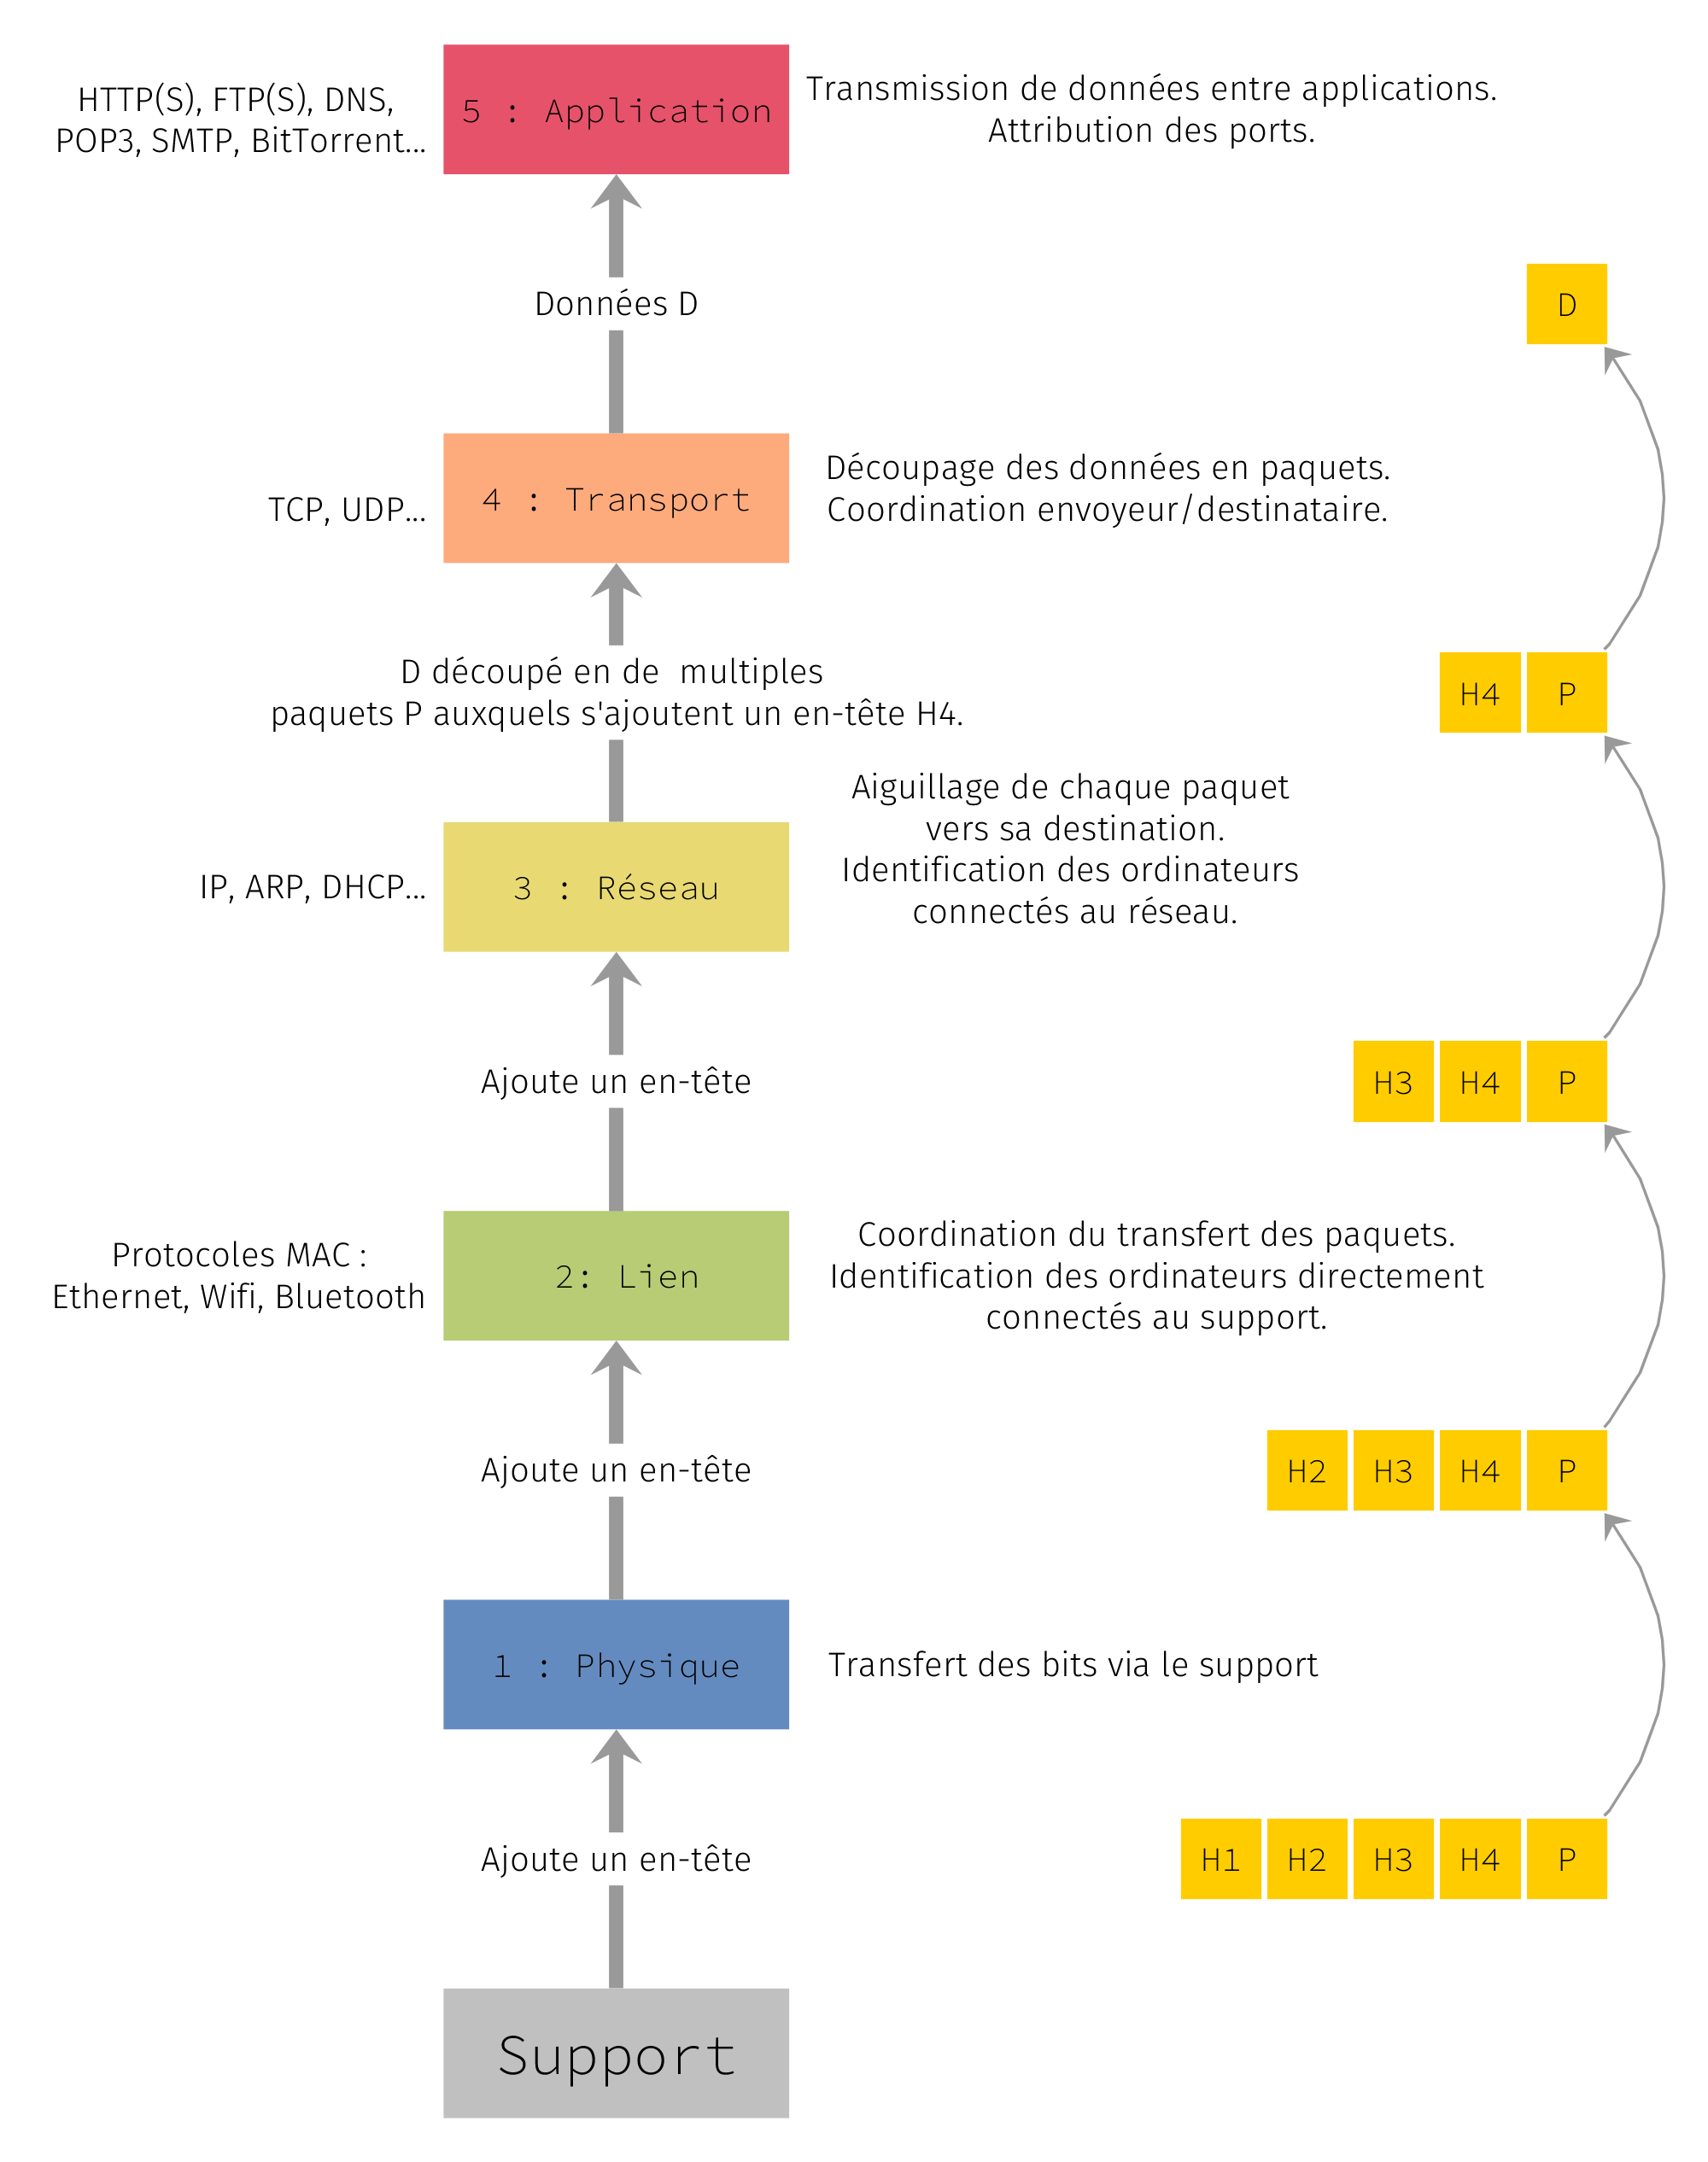
\includegraphics[width=10cm]{ch-reseaux/img/modele_5_couches_up.png}\\
        
            \footnotesize{Enchaînement des opérations du point de vue de l'émetteur}
        \end{center}

\textbf{Couche 4 - Transport :} Cette couche va découper les données fournie par la couche 5 en paquets (d'une taille de l'ordre du kilooctet). Elle ajoute également son propre en-tête à chaque paquet.\\
          Les protocoles les plus connus sont
          \begin{itemize}
              \item 	TCP (\textit{Transfert Control Protocol}), protocole de contrôle des transmissions, qui est fiable, fonctionne sur le principe d'une connexion avec accusé de réception.
              \item 	UDP (\textit{User Datagram Protocol} ), non fiable en théorie, sans connexion ni accusé de réception, mais plus rapide.
          \end{itemize}
          On utilise TCP lorsque les données à recevoir sont sensibles (téléchargement d'un fichier). UDP sera préféré dans le cas du \textit{streaming} : le protocole est plus rapide et permet par exemple de visionner un film avec une bonne qualité, et si des données sont perdues, ce n'est pas grave, on passe aux données suivantes, cela ne perturbe pas trop le film (on ne va pas, comme ce serait le cas pour TCP, attendre que les données soient arrivées, et faire des pauses).\\

\textbf{Couche 3 - Réseau :} Cette  couche est responsable de l'aiguillage des paquets vers l'adresse de destination. Elle encapsule les paquets de la couche 4 et y ajoute son propre en-tête (en général un en-tête IP). Du point de vue de cette couche, les paquets sont à envoyer à un ordinateur muni d'une adresse IP (nombre attribué par ce protocole).\\ Pour que les paquets trouvent leur chemin de l'ordinateur A à l'ordinateur B (qui peut être à plusieurs milliers de kilomètres de A), de \textit{protocoles de routage sont utilisés}, les machines dédiées au routage s'appellent des \textit{routeurs}. Un routeur n'utilise que les couches 1,2 et 3 du modèle.\\
          Il faut retenir que chaque paquet suit son propre chemin, indépendamment des autres et qu'il a un « temps de vie » (pour éviter, s'il est perdu, de circuler sur le réseau pendant des années).\\
          Parmi les protocoles utilisés par cette couche on trouve
          \begin{itemize}
              \item 	IP (\textit{Internet Protocol}), décrit ci-dessus ;
              \item 	ARP (\textit{Address Resolution Protocol}) qui permet de trouver l'adresse \textit{physique} de l'ordinateur connecté à l'adresse IP. Ce protocole est utilisé lorsque l'information est arrivée à B et « remonte les couches ».\\
          \end{itemize}

\textbf{Couche 2 - Lien :} Elle est chargée de coordonner le transfert des données ainsi que le « temps de parole » de chaque machine connectée au support physique (si toutes les machines connectées à un même support émettent des données en même temps, il risque d'y avoir des \textit{collisions}). Elle encapsule les paquets de la couche supérieure dans ce qu'on appelle des \textit{trames} (trames Ethernet par exemple).\\
          Du point de vue de la couche lien, la destination d'un paquet est une adresse physique appelée adresse MAC (Media Access Control), déterminée par la carte réseau de la machine destinataire.
          Les protocoles utilisés par cette couche sont Ethernet (réseau filaire), Wi-Fi (réseau \textit{via} les ondes.\\
\textbf{Couche 1 - Physique :} Elle est chargée de la transmission effective des trames (qu'elle encapsule également) d'un bout à l'autre du support physique.


\subsection{Du point de vue du récepteur}

Il faut retenir que chaque couche dépaquète le paquet (ou trame) qui lui est adressé en enlevant l'en-tête correspondant et passe le relais à la couche du dessus.

\begin{center}
    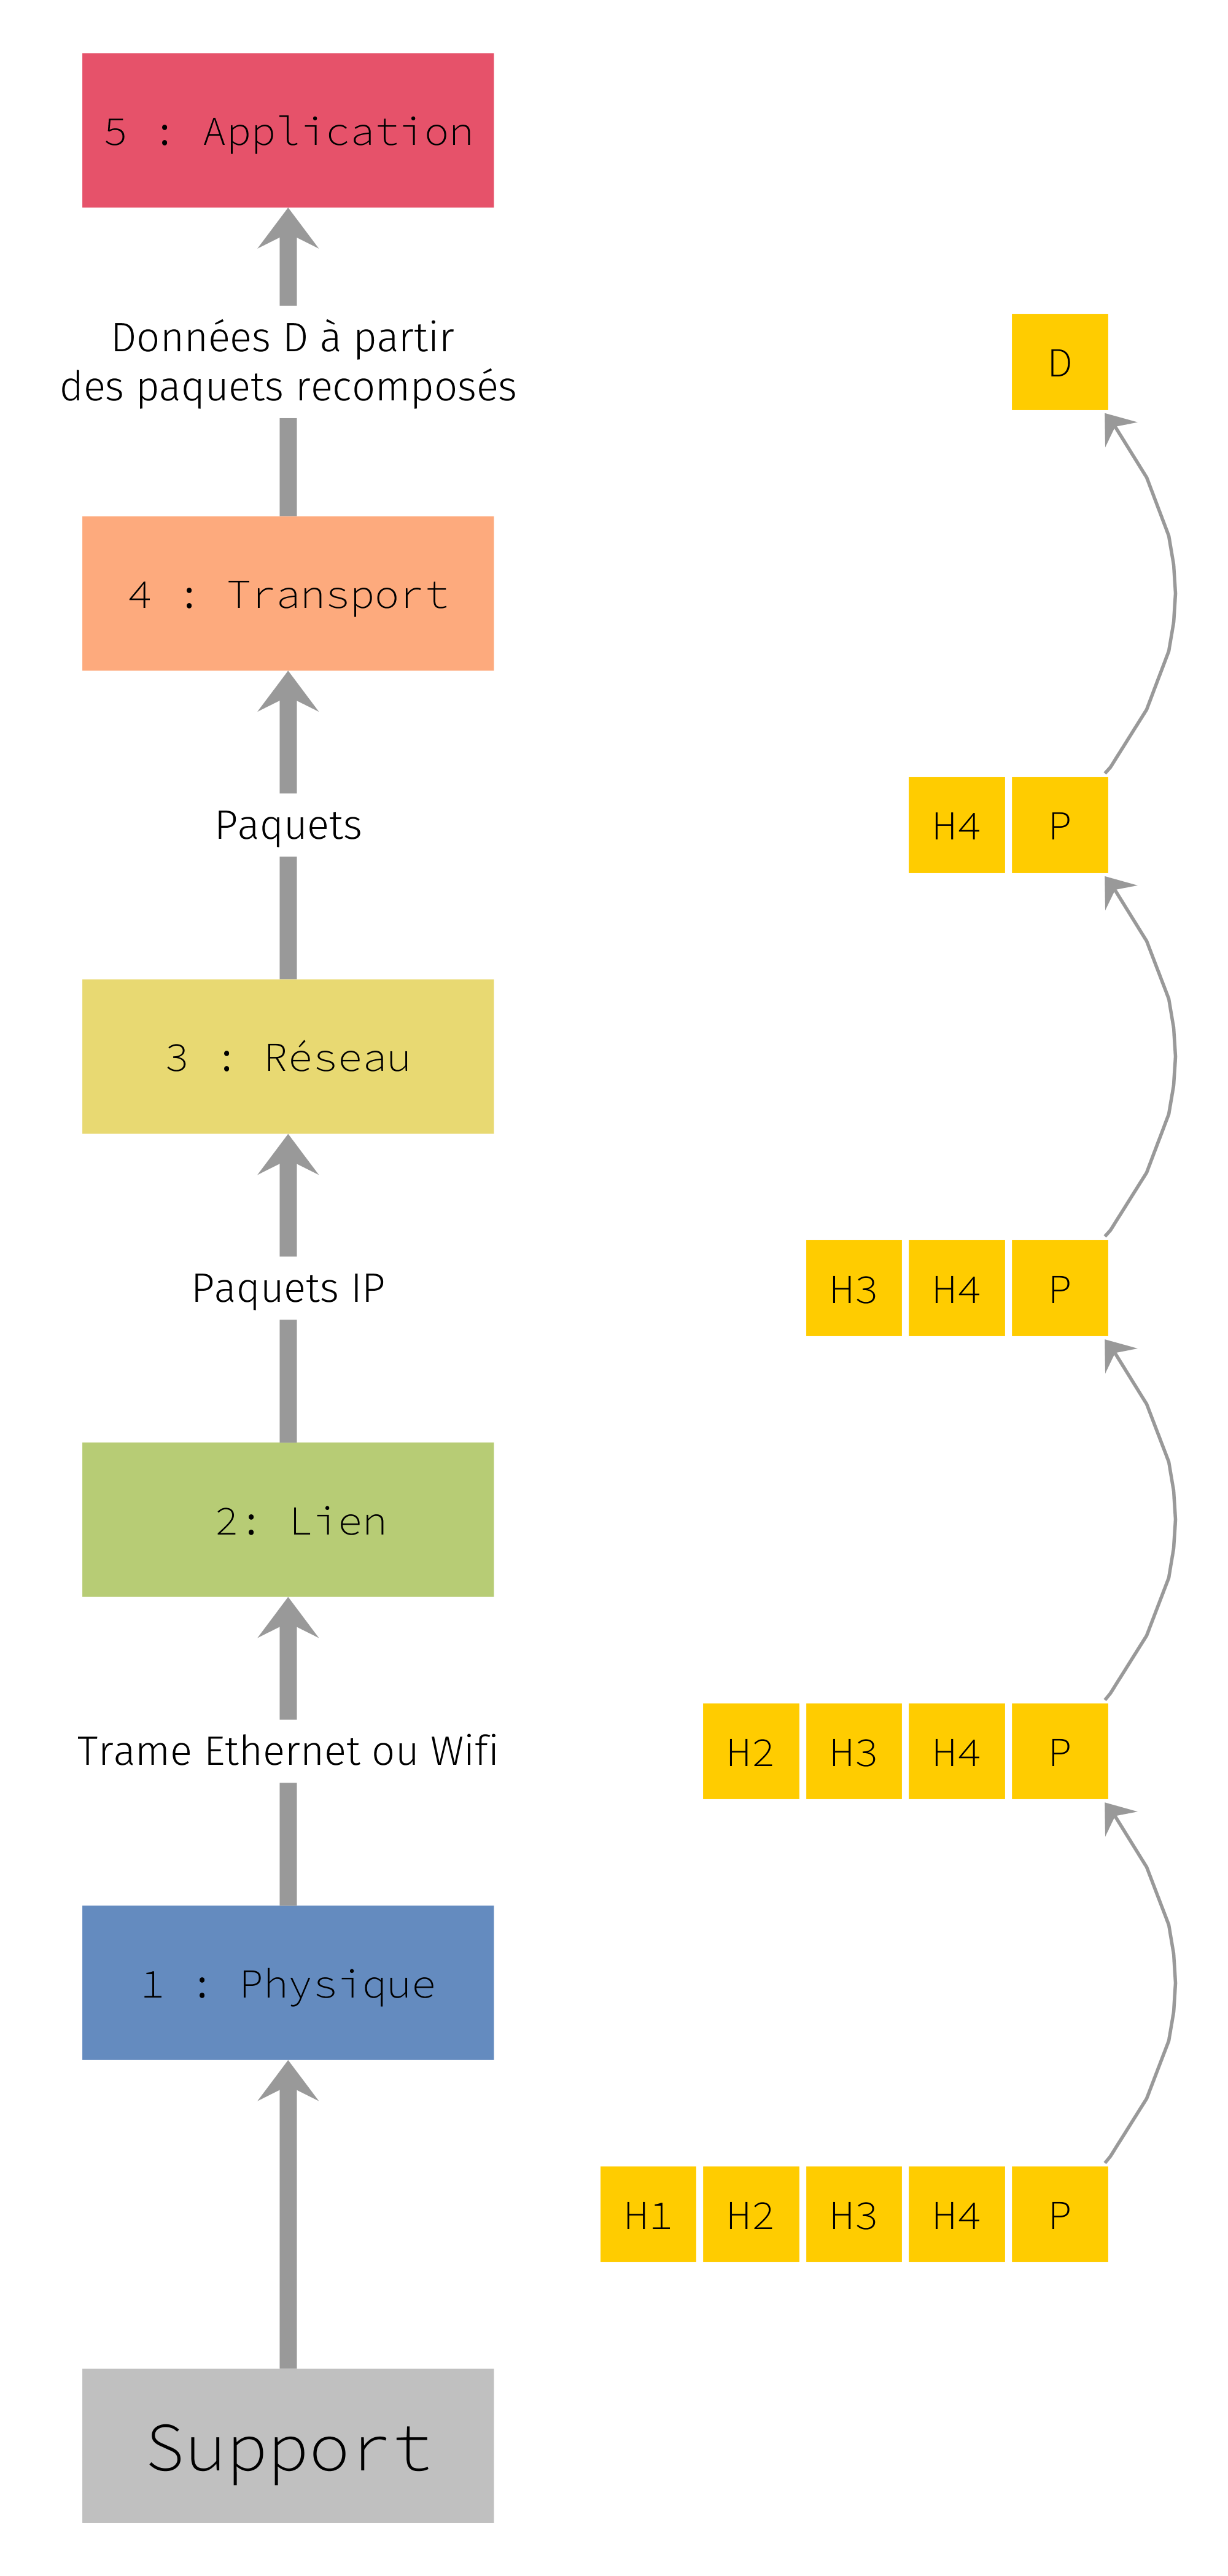
\includegraphics[width=6cm]{ch-reseaux/img/modele_5_couches_down.png}\\
    \footnotesize{Enchaînement des opérations du point de vue du destinataire}
\end{center}
\section{Le matériel}

\subsection{Couche physique }

\subsubsection{Liaison filaire}

\floatpictureright{0.3}{ch-reseaux/img/cable_ethernet}{
    Les informations peuvent être transmises \textit{via} des câbles. Le plus utilisé est le câble Ethernet. Son nom est UTP-CAT5 ou UTP-CAT6, la différence étant que le second permet un débit dix fois plus grand que le premier ( 1 Gbit/s contre 100 Mbit/s).\\
    Parmi les autres types de liaisons filaires, on compte la liaison par câble téléphonique (qui permet par exemple de se connecter à Internet par ADSL) et la liaison par câble optique.
}

\subsubsection{Bluetooth}
\floatpictureleft{0.15}{ch-reseaux/img/logo_bluetooth.png}{
    C'est une technologie utilisant les ondes radios pour permettre la communication entre les équipements électroniques (imprimantes, téléphones, scanners, système audio portatif ou dans un véhicule...) à courte distance. Ses fonctionnalités sont assez limitées en terme de mise en réseau.}

\subsubsection{Wi-Fi}

\floatpictureright{0.3}{ch-reseaux/img/logo_wifi}{
    Cette technologie utilise également les ondes radio. Son nom de norme est IEEE 802.11 et c'est le moyen de transmission des données sans fil le plus utilisé.}

\subsubsection{Répéteur et concentrateur}

Lorsqu'un signal parcourt le support physique, son intensité s'atténue avec la distance. Un \textit{répéteur} régénère le signal perçu avec plus d'intensité pour pallier ce problème.\\
Le concentrateur (hub) est moins utilisé de nos jours. C'est une version « multiprise » du répéteur : quand il reçoit un signal sur un des ses branchements, il les recopie sur tous les autres branchements sans se soucier de l'éventuel destinataire du signal.

\subsubsection{Carte réseau}


\floatpictureleft{0.3}{ch-reseaux/img/carte_reseau}{
    Que ce soit une clé USB Wi-Fi ou une carte réseau interne, c'est la même chose : ce composant est indispensable pour connecter un ordinateur à un réseau.\\
    Chaque carte réseau possède une \textit{adresse MAC} : c'est l'adresse physique de la carte, elle permet d'identifier l'ordinateur de manière unique.}

\subsection{Couche lien}
\floatpictureright{0.3}{ch-reseaux/img/switch}{
    Le \textit{concentrateur} (\textit{switch} en Anglais) est un équipement à plusieurs branchements (au moins 2) appelés \textit{ports} (ne pas confondre avec la notion de port utilisé par une application).\\
    Son rôle est de rediriger une trame reçue vers l'ordinateur de destination.}

\subsection{Couche réseau}

\floatpictureleft{0.3}{ch-reseaux/img/routeur}{
    Le \textit{routeur} (\textit{router} en Anglais) permet d'effectuer le routage des paquets et de les faire transiter d'une partie du réseau vers une autre (par exemple d'un réseau local à un autre, nous verrons cela plus tard).}


\subsection{Couches supérieures}

C'est un ordinateur qui exécute les protocoles des couches transport et application. Cela peut être un téléphone, une tablette, un ordinateur portable ou de bureau ou bien encore un objet connecté tel qu'une enceinte Bluetooth.
%  \chapter{Le réseau local}
Un \textit{réseau local}, ou LAN (\textit{Local Area Network}) est de taille modeste. Les équipements qui y sont connectés s'envoient des données entre eux sans passer par internet. Un bon exemple de LAN est le \textit{réseau domestique} d'une maison :
\begin{itemize}
    \item    la box, fournie par l'opérateur (Orange, Free, Bouygues...) fait office de switch et de routeur;
    \item    les téléphones portables, tablettes, ordinateurs, imprimantes et autres s'y intègrent.
\end{itemize}
\begin{center}
    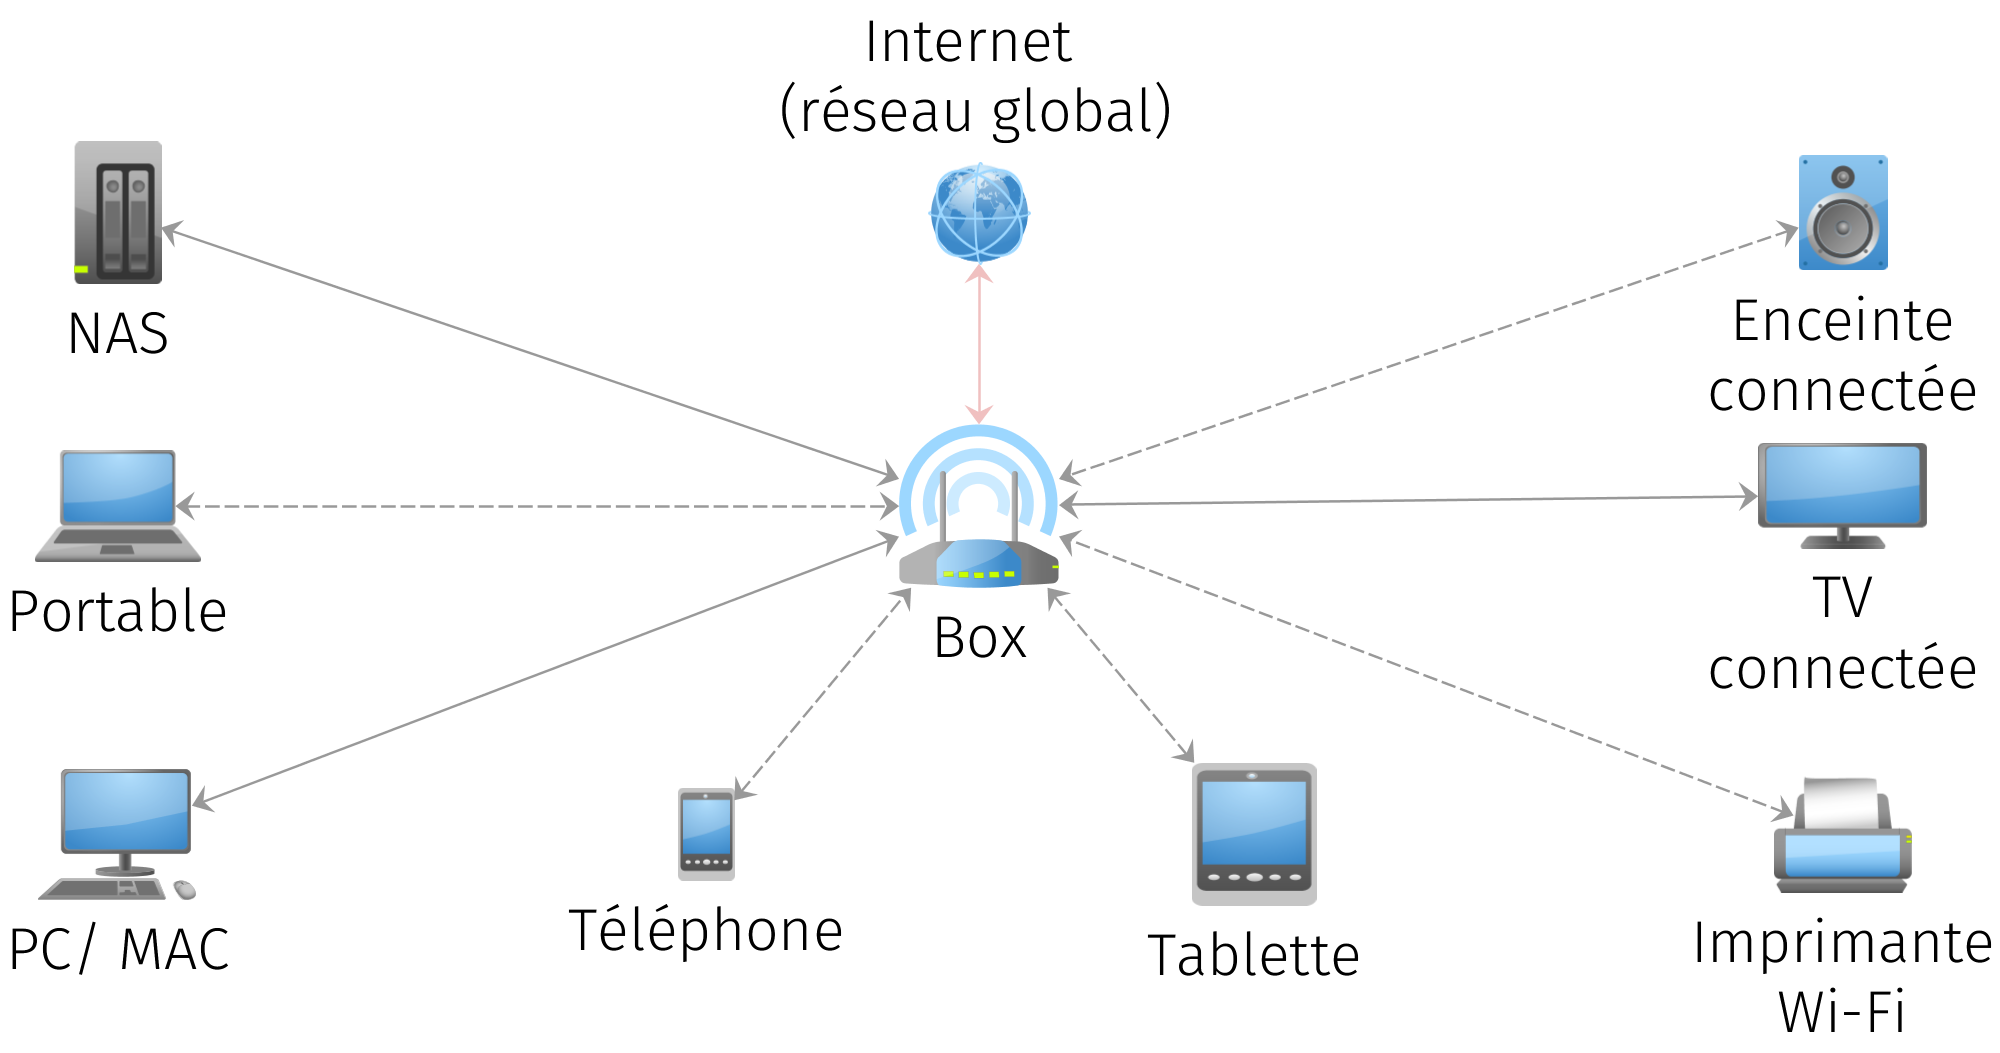
\includegraphics[width=\textwidth]{ch-reseaulocal/img/reseau_local.png}
\end{center}

\section{Les adresses IP privées et publiques}
On a vu dans le chapitre précédent l'importance de l'adresse IP d'un ordinateur dans le rôle de la communication.

\begin{definition}[ : adresse IPv4]
    Une adresse IP (version 4) est la donnée de 4 octets. On les note séparés par des points. Il y a 5 classes d'adresse IP, notées A, B, C, D et E et les 3 premières classes disposent d'adresses IP (on abrègera en IP) publiques et privées.
\end{definition}

\begin{exemple}[s]
    \begin{itemize}
        \item    74.125.21.138 est à ce jour une IP permettant d'accéder au site du moteur de recherche de Google. C'est une IP \textit{publique}, accessible par tout le monde \textit{via} Internet.\\
        \item    192.168.1.47 est l'IP de l'ordinateur sur lequel j'écris ces lignes. C'est une IP \textit{privée} : elle n'est accessible que par les ordinateurs de mon propre réseau domestique. Elle n'est d'ailleurs pas \textit{unique} non plus dans le sens où d'autre réseaux domestiques utilisent cette IP.
        \item    lorsque je veux voir mon IP publique, je vais par exemple consulter \texttt{http://whatismyip.host/} et je trouve une adresse différente : 83.199.117.xx (permettez moi de garder mon adresse IP secrète).
    \end{itemize}
\end{exemple}

Une adresse IP publique, c'est un peu comme une adresse postale publique : elle identifie de manière unique une machine (qui peut être une box jouant le rôle de routeur vers un réseau domestique).\\
Une adresse IP privée, c'est un peu comme le numéro et le nom de la rue sans la ville ni le pays : il y a sans doute beaucoup d'adresse au 24 rue des oliviers. Si le réseau postal ne concerne que la ville de Rennes, cette adresse est suffisante, mais si je cherche à envoyer du courrier au 24 rue des oliviers, cela ne marchera pas.

\begin{remarque}[s]
    \begin{itemize}
        \item    4 octets pour une adresse IP, c'était bien il y a 30 ans, ça l'est beaucoup moins de nos jours !\\ $2^{32}=\np{4 294 967 296}$, donc vu le nombre de machines croissant en fonctionnement simultané sur Terre, il est impossible d'attribuer une IP unique à chaque ordinateur connecté à Internet, d'où l'importance du LAN.

        \item    Pour pallier le problème, une norme IP version 6, plus performante, sur 128 bits au lieu de 32, a vu le jour mais peine encore à s'imposer.
    \end{itemize}
\end{remarque}

Voici les plages d'IP publiques et privées selon les classes :
\begin{itemize}[]
    \item    \textbf{Classe A :} de l'adresse IP 0.0.0.0 à 126.255.255.255.\\
          Adresses privées : de 10.0.0.0 à 10.255.255.255 (avec 16 millions d'adresses possibles au sein d'un réseau local).

    \item    \textbf{Classe B :} de l'adresse IP 128.0.0.0 à 191.255.255.255.\\
          Adresses privées : 172.16.0.0 à 172.31.255.255 (avec 65535 adresses possibles au sein d'un réseau local).
    \item    \textbf{Classe C :} de l'adresse IP 192.0.0.0 à 223.255.255.255.\\
          Adresses privées C : 192.168.1.0 à 192.168.255.255 (255 adresses possibles dans un réseau local).
    \item    \textbf{Classe D (réservée) :} de l'adresse IP 224.0.0.0 à 239.255.255.255.
    \item    \textbf{Classe E (réservée) :} de l'adresse IP 240.0.0.0 à 255.255.255.255.
\end{itemize}

\begin{exemple}[]
    Mon adresse IP publique est une IP de classe A, mon IP privée est de taille C, ce que je comprends parfaitement puisque mon réseau domestique ne contiendra qu'une dizaine de terminaux tout au plus.
\end{exemple}


\section{L'exemple du réseau local traditionnel}

Lorsqu'on met en place un réseau local, on commence par déterminer sa taille. Il y a beaucoup de chances qu'on ait moins de 256 machines à connecter donc on va choisir une IP publique de classe C :
\begin{itemize}
    \item    je choisis de prendre pour \textit{adresse réseau} 192.168.1.0, ce n'est pas une IP attribuée à une machine, elle désigne mon réseau local ;
    \item    le \textit{masque de sous-réseau} par défaut est 255.255.255.0, ce qui signifie que les 3 premiers octets des machines de mon réseau sont « bloqués » et donc que les machines vont avoir des adresses du type 192.168.1.xx ;
    \item    je peux attribuer des IP aux machines que je veux connecter, par exemple 192.168.1.1 pour la première, et c\ae tera ;
    \item    la dernière IP 192.168.1.255 est interdite, elle est réservée pour adresser un message à l'ensemble des machines du réseau (on appelle ceci \textit{broadcast}).
\end{itemize}

\begin{remarque}[]
    Prenons le cas d'un foyer qui utilise le FAI Orange. Par défaut le réseau local est 192.168.1.0. avec pour masque 255.255.255.0. La LiveBox, qui fait office de switch et de routeur, a pour adresse 192.168.1.1. C'est cette adresse qui est utilisée comme passerelle pour accéder à internet :
    \begin{center}
        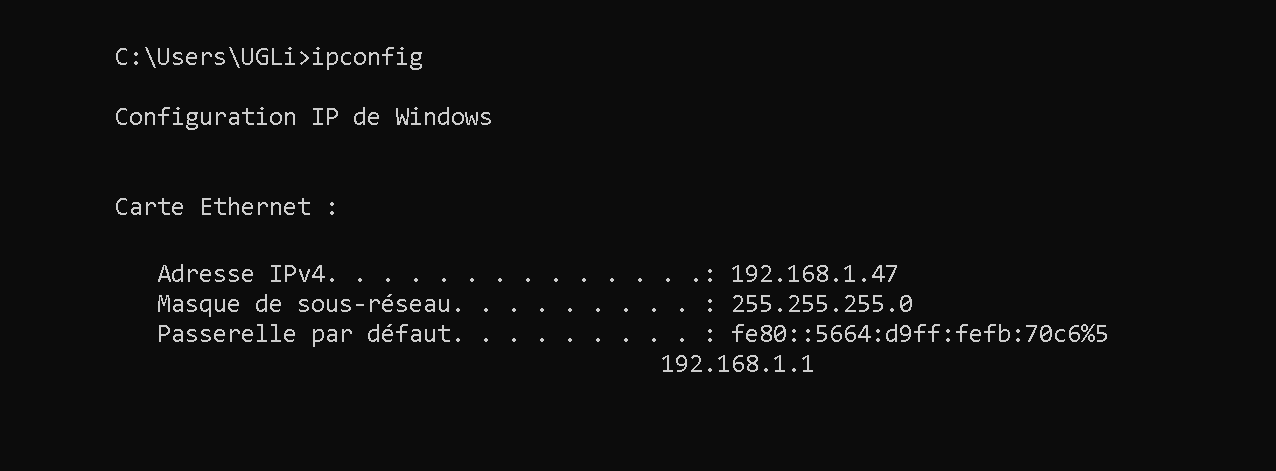
\includegraphics[width=\textwidth]{ch-reseaulocal/img/ipconfig.png}
    \end{center}

    La commande\texttt{ipconfig} de Windows (\texttt{ifconfig} sous Linux et Mac) me permet de retrouver ces informations ainsi que mon IP privée.
\end{remarque}
\begin{exercice}[]
    Utilise l'invite de commande de ton système d'exploitation (touche windows et taper\texttt{cmd} pour Windows, Terminal sous MacOS) et trouve l'IP de ton ordinateur, le masque de sous-réseau et l'adresse de la passerelle.
\end{exercice}
\section{Un outil de simulation réseau : Filius}

Filius est un logiciel libre fonctionnant sur tous les systèmes d'exploitation et permettant de simuler le fonctionnement d'un petit réseau. On peut
\begin{itemize}
    \item    ajouter du matériel : ordinateur, switch, routeur et modem;
    \item    connecter les éléments précédents;
    \item    configurer ces éléments;
    \item    installer de petites applications sur les ordinateurs connectés pour transmettre ou recevoir des données sur le(s) réseau(x).
    \item    visualiser les échanges de données.
\end{itemize}

Nous utiliserons Filius pour observer ce que nous avons appris des réseaux.



%  \chapter{Contrôles de transmission}

\section{Le protocole du bit alterné}

Nous allons ici voir un modèle de \textit{contrôle de perte de données} appelé \textit{protocole du bit alterné}.
Ce protocole a (ou plutôt avait car il a été remplacé par un protocole plus performant) lieu au sein de la couche 2 (couche lien) et permet de vérifier que les trames d'un ordinateur A sont bien reçues par un ordinateur B.\\

Le principe est très simple, il utilise les \textit{acquittements} et les \textit{flags} :  lorsque A envoie une trame, il attend un accusé de réception (acquittement, \textit{acknowledgment} en Anglais) de la part de B dans un temps imparti.\\ À ceci s'ajoute un bit de contrôle, appelé \textit{flag} en Anglais, qui alterne suivant le modèle suivant:\\

\floatpictureright{0.4}{ch-transmissions/img/bit_alterne_1}{
    \begin{itemize}
        \item 	la communication commence avec le \textit{flag} à 0, A envoie une première trame avec le \textit{flag} ;
        \item 	B reçoit la trame et accuse réception en envoyant une trame d'acquittement notée ACK. le \textit{flag} est changé à 1 ;
        \item 	A reçoit ACK avec le flag 1 et envoie donc la 2\eme trame avec ce \textit{flag} 1 ;
        \item 	et ainsi de suite : Lorsque A reçoit une trame de B, elle garde la valeur du \textit{flag} pour la prochaine trame qu'elle envoie.B, quant à lui change toujours le \textit{flag} entre le moment où il reçoit et celui ou il émet.
    \end{itemize}
}

Ce protocole permet d'éviter la perte de trames dans les cas suivants :\\

\floatpictureleft{0.4}{ch-transmissions/img/bit_alterne_2}{
    \subsection{Perte de trame du côté de A}
    A envoie la première trame et celle-ci se perd, au bout du temps imparti, ne reçoit rien.\\
    C'est ce qu'on appelle un \textit{timeout} en Anglais.\\
    A renvoie donc sa trame comme si de rien n'était.}\medskip\par

\floatpictureright{0.4}{ch-transmissions/img/bit_alterne_3}{
    \subsection{Perte de trame du côté de B} A envoie la première trame et celle-ci arrive à B, qui renvoie un ACK avec un \textit{flag} à 1, et s'attend donc à recevoir une prochaine trame avec un \textit{flag à 1}.\\
    Cette trame ACK se perd donc du point de vue de A, il y a \textit{timeout} et donc il renvoie la même trame avec le \textit{flag} à 0. B se rend compte que quelque chose ne va pas, et renvoie donc l'ACK précédent, avec son \textit{flag} à 1. La communication continue normalement.}\medskip\par

Ce protocole présente des insuffisances comme le montre l'exercice suivant

\begin{exercice}[]
    Analyse le schéma suivant et explique pourquoi il y a perte d'information.
    \begin{center}
        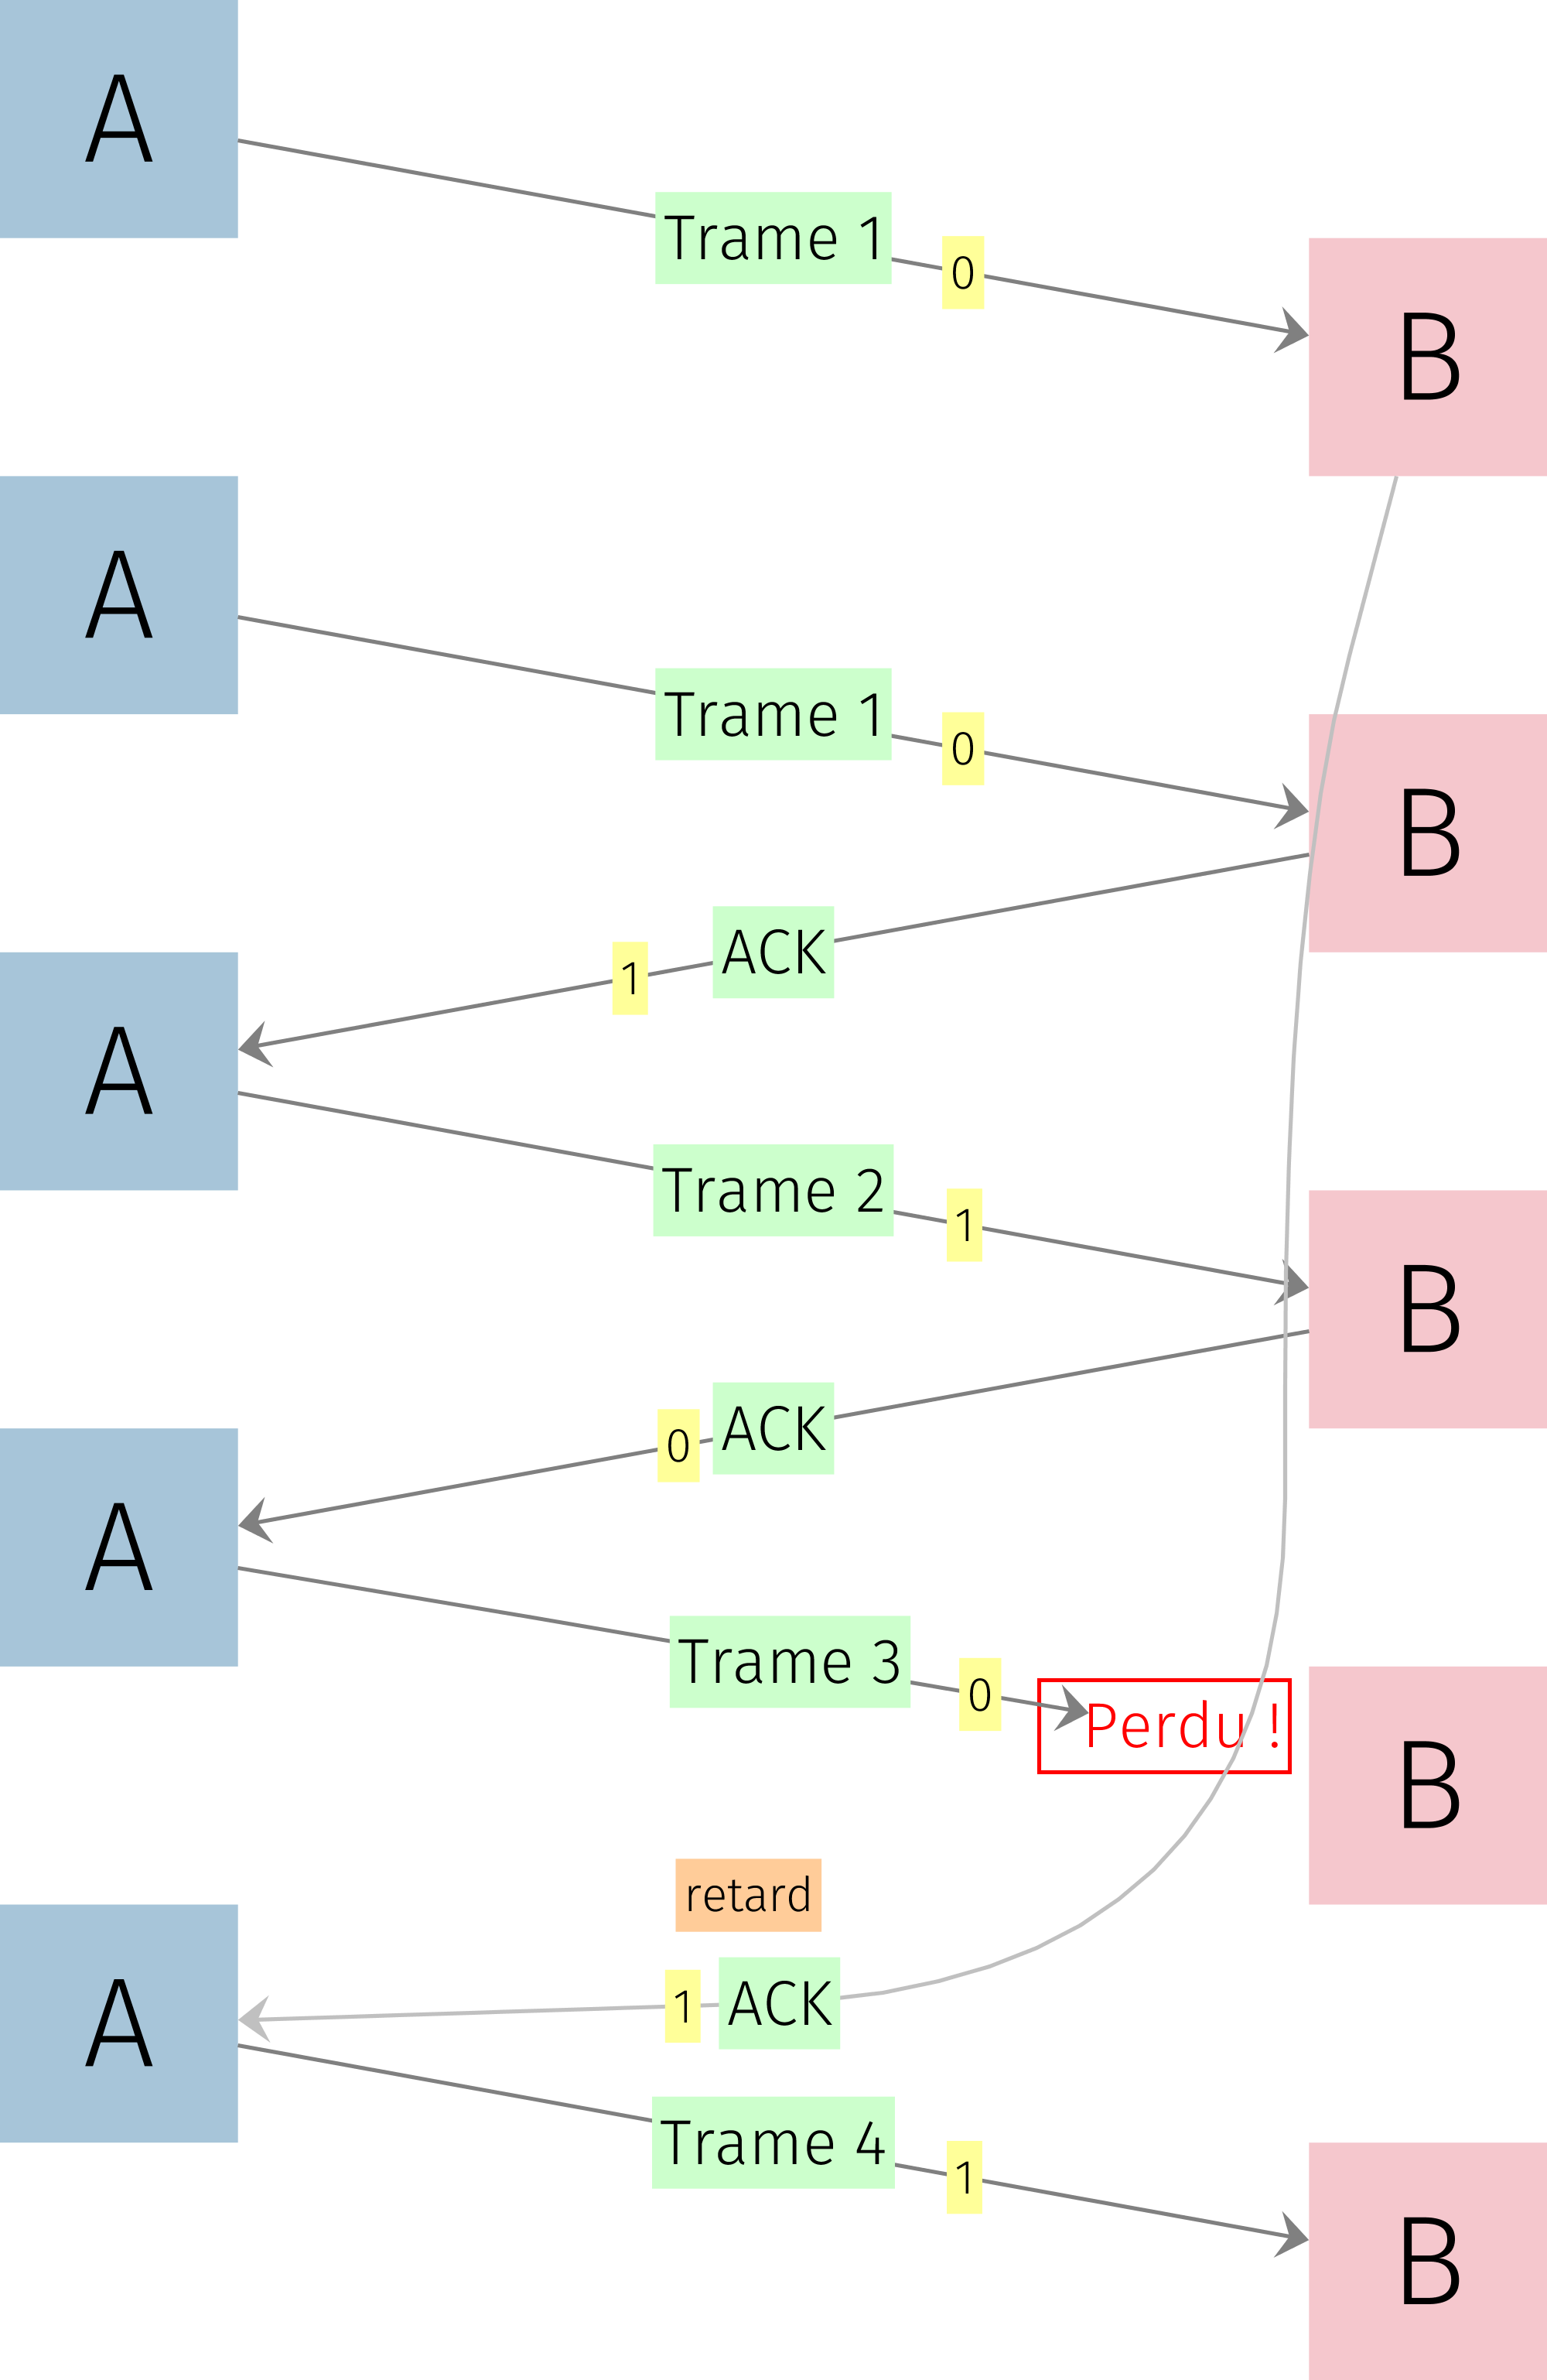
\includegraphics[width=4.2cm]{ch-transmissions/img/bit_alterne_4.png}
    \end{center}
\end{exercice}

\section{Déroulement d'une communication TCP}

On rappelle que TCP est un protocole de la couche 4 (couche transport) dont les caractéristiques principales sont les suivantes :
\begin{itemize}
    \item 	il commence par établir une connexion entre les deux machines ;
    \item 	il découpe les données en paquets ;
    \item 	il s'assure de la bonne réception des données au moyen d'\textit{accusés de réception} ;
    \item 	il met fin à la connexion.
\end{itemize}

L'exercice suivant va nous permettre d'examiner une exemple de communication TCP en détail.

\begin{exercice}[]
    Reprendre le fichier Filius de l'exercice 5 (serveur web avec DNS ) de la feuille de TP sur Filius.
    \begin{enumerate}
        \item 	En mode simulation, faire un clic droit sur 192.168.2.1 et afficher les échanges de données.
        \item	Normalement il n'y a encore eu aucune communication réseau donc la fenêtre d'échange est vide.\\
              Sur le navigateur web installé sur 192.168.2.1, entrer \texttt{monsite.com} et observer la fenêtre d'échange de données \textit{du point de vue de 192.168.2.1} :
              \begin{center}
                  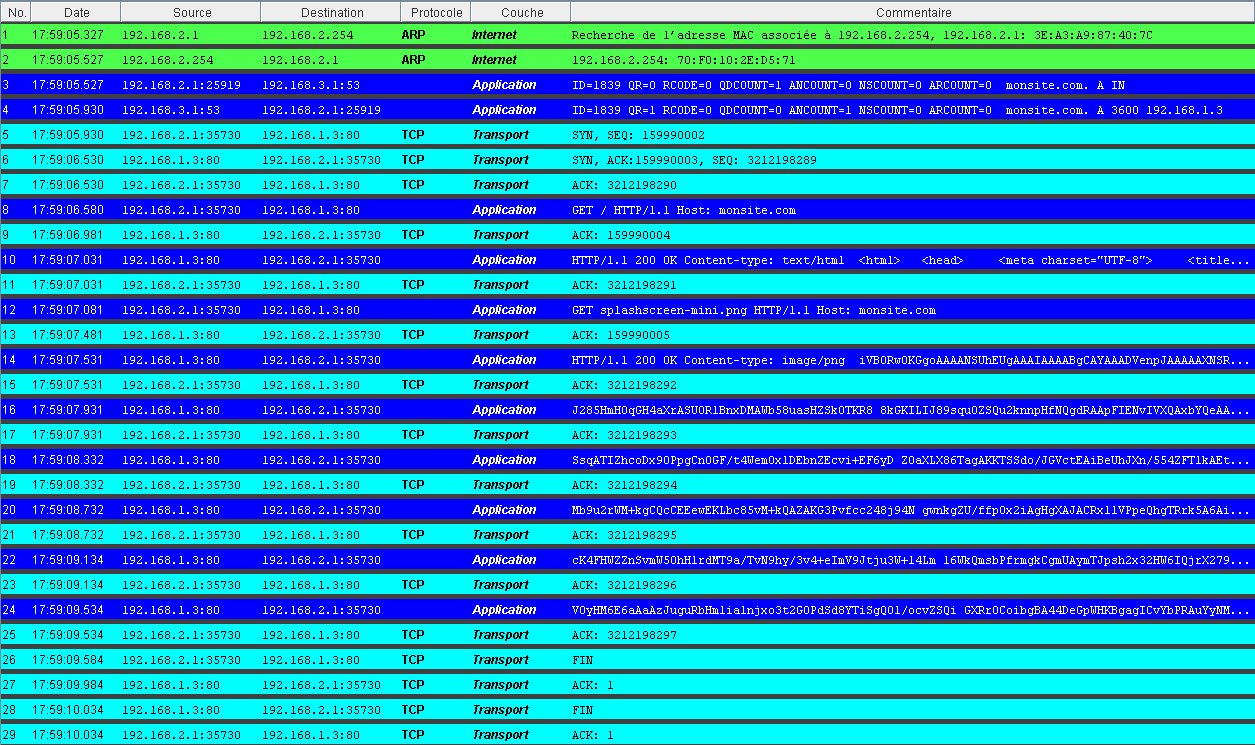
\includegraphics[width=\linewidth]{ch-transmissions/img/echange_donnees.png}
              \end{center}
              On observe 29 trames. Il est possible de cliquer sur chacune d'entre elles pour visualiser son contenu. Voici le contenu de la première :
              \begin{center}
                  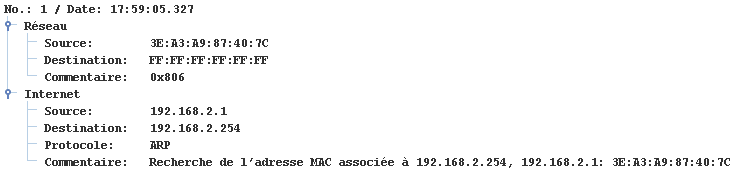
\includegraphics[width=\linewidth]{ch-transmissions/img/trame_1.png}
              \end{center}
              Il nous indique que 192.168.2.1 essaie de déterminer l'adresse MAC du routeur. En effet, 192.168.2.1 doit interroger le serveur DNS, situé en 192.168.3.1, pour obtenir l'adresse IP associée à \texttt{monsite.com}, et puisque 192.168.3.1 , n'est pas dans le même réseau que 192.168.2.1, celui-ci utilise la passerelle (le routeur).\\
              La trame suivante est la réponse ARP et la communication se poursuit.
    \end{enumerate}
    \begin{enumerate}
        \item 	Regarder la source, la destination et le contenu des trames 3 et 4. À quoi correspondent-elles ?
        \item 	On s'intéresse au début de la connexion TCP de 192.168.1.2.1 à 192.168.3.1 : ce sont les trames 5,6 et 7, qui constituent ce qu'on appelle en Anglais un \textit{Three-way handshake}. Rechercher ce terme sur Wikipédia et interpréter ensuite les 3 trames.
        \item 	Les trames 8 à 25 constituent l'échange de données en lui-même. Il y a deux grandes étapes. Lesquelles ?
        \item 	Que représentent les trames 26 à 29 ? Détailler le procédé.
    \end{enumerate}
\end{exercice}


 \part{Le Web}
\end{document}